\documentclass{nicksclass}

\includeonly{%Easy include/exclude of chapters
abstract,%
intro%
,
nestedSampling%
,
flowering%
,
discussion%
}

\begin{document}
\DeclareFieldFormat[article,book,manual,inproceedings,incollection,thesis,online]{title}{\mkbibbold{#1}}% Bold titles in Bibliography
\DeclareFieldFormat[article]{titlecase}{\MakeSentenceCase{#1}}
\strictpagecheck% For ouside margins

% Title page
\thispagestyle{empty}
\newgeometry{textheight=706pt, marginparsep=0pt, marginparwidth=0pt, textwidth=400pt, inner=98.753pt}%So inner = outer ergo text can be centred on page
\myTitlePage
\restoregeometry
\thispagestyle{empty}

% Abstract
\cleardoublepage
\thispagestyle{empty}
\phantomsection% Needed for hyperref to link correctly
\addcontentsline{toc}{chapter}{Abstract}
\chapter*{Abstract}
Flowering plants are abundant on Earth.
In the model dicot plant species, \emph{Arabidopsis thaliana}, multiple endogenous and exogenous signals converge to initiate a change from vegetative to reproductive growth in optimal environmental conditions.
Much genetic and experimental research has gone into elucidating the biological mechanisms controlling the floral transition.
However there has been little mathematical modelling of this process.

The aim of this thesis was to gain an understanding of the essential features and dynamic properties underlying this developmental phase change from a systems and computational biology perspective.
Combining mathematical modelling with experimental results a core regulatory network was defined with multiple feedback loops.
Simplified models inevitably miss finer details of the biological system yet they provide a route to understanding the overall system behaviour.
This reductionist path allowed a tractable genetic regulatory network to be investigated without large numbers of parameters.

Not overfitting to data and parameter inference are two current challenges in systems biology.
Treating all unknowns as a probability within the setting of Bayes' theorem as a statistical framework allows for a solution to both of these issues.
This thesis investigates the use of a contemporary Bayesian inference algorithm, nested sampling, for inference problems typically found in systems biology where the data are few and noisy.
Nested sampling simultaneously calculates the key term for model comparison and also produces parameter inferences allowing uncertainty in models and predictions to be robustly quantified.

Network models are developed that can accurately reproduce experimental leaf number data, show important properties of the floral transition such as the ability to filter environmental noise and provide a clue on spatial patterning of an Arabidopsis shoot apex.
Incorporating network knowledge into a plant breeding program is an exciting goal for future developments addressing global food security.
\thispagestyle{empty}
% only clearpage gets rid of following header
\clearpage
\thispagestyle{empty}

% ToC
{\hsize 441pt
\tableofcontents
\cleardoublepage}

% My publications
\phantomsection% Needed for hyperref to link correctly
\addcontentsline{toc}{chapter}{List of publications}
\chapter*{List of Publications}
  This thesis includes material from the published works below.\newline
  * Indicates that these authors contributed equally.

\vspace{1cm}\noindent
A. Bentley, E. Jensen, I. Mackay, H. Hönicka, M. Fladung, K. Hori, M. Yano, J. Mullet, I. Armstead, C. Hayes, D. Thorogood, A. Lovatt, R. Morris, N. Pullen, E. Mutasa-Göttgens, and J. Cockram. \textbf{Flowering Time}. In: \emph{Genomics and Breeding for Climate-Resilient Crops: Vol. 2 Target Traits} (2013), 1--66.

\vspace{1cm}\noindent
K. E. Jaeger*, N. Pullen*, S. Lamzin, R. J. Morris, and P. A. Wigge. \textbf{Interlocking feedback loops govern the dynamic behavior of the floral transition in \emph{Arabidopsis}}. \emph{The Plant Cell} 25.3 (2013), 820--833

\vspace{1cm}\noindent
N. Pullen, K. E. Jaeger, P. A. Wigge, and R. J. Morris. \textbf{Simple network motifs can capture key characteristics of the floral transition in \emph{Arabidopsis}}. \emph{Plant Signaling \& Behavior} 8.11 (2013), e26149.

\vspace{1cm}\noindent
N. Pullen and R. J. Morris. \textbf{Bayesian model comparison and parameter inference in systems biology using nested sampling}. \emph{PLoS ONE} 9.2 (2014), e88419.
\thispagestyle{empty}

% only clearpage gets rid of following header
\clearpage
\thispagestyle{empty}
\chapter*{Acknowledgements}
\chaptermark{Acknowledgements}% So correct name appears in header
\addcontentsline{toc}{chapter}{Acknowledgements}
I would like to thank my main supervisor Richard Morris for all the support he has given me throughout these long, and sometimes trying, four years.
I appreciate his giving me the opportunity to study for a PhD in his group and for allowing me to attempt to combine my mathematical knowledge with my interest in plants.
He has been full of useful suggestions, especially when things did not turn out as expected in this project.
His good humour and scientific integrity have been sterling examples for me to follow in the future.
I also thank Richard a lot for comments on draft chapters of this thesis which have improved it considerably.

I would like to thank all the post-docs and students in the Computational \& Systems Biology department who have been a great group to spend my time with.
In particular I'd like to acknowledge the help of David Richards in the early days for getting me up and running with learning Linux and Python.
He also orchestrated much lunchtime entertainment which I think provide many of us with fond memories.
I owe a lot of thanks to Matthew Hartley who joined CSB as our lab manager and was able to give me lots of hints on computing and programming.

Other members of my supervisory team deserve mentions.
Phil Wigge and Katja Jaeger provided the experimental angle of the project and I thank them for the leaf number data, and helping choose me to do a PhD at JIC\@.
Rico Coen also provided food for thought throughout the project and allowed us the benefit of his wisdom.

I am indebted to the Brassica tendency crew of Marc Jones, Rachel Wells, Judith Irwin, Martin Trick and Colin Morgan for making the final year of my PhD the most enjoyable one.
We've had many fun meetings, social occasions and they have allowed me to finally enter the greenhouses to see growing plants close up.
I also thank Judith for some useful comments on chapter 3.

It was also good to meet lots of people on the various training courses or conferences I attended all over Britain and Europe.
Their enthusiasm showed me a good view of science and the wider world.
I should also acknowledge lots of online bloggers and communities whose various tips saved me (or sometimes caused me!) much frustration at the keyboard.
Principally those who have, and continue to contribute to \url{StackOverflow.com} or \url{tex.stackexchange.com} have been incredibly valuable to my development as someone who can now program a fair bit.

In Norwich, I thank Glen and Annika Richardson for letting me lodge in their lovely house for the first nine months of my PhD.
Thereafter I thank Steve Garrett for being my landlord in a friendly house very close to work.
To the members of the UEA Athletics and Hockey Clubs I was a member of during my PhD years I am indebted to helping me keep it real, and reminding me life isn't all about about long hours in front of the office computer.
It was an honour to serve as UEAHC Club Captain and to help coach the distance athletes from UEAAC\@.

I feel very lucky to have met Yan Ma who has shown much kindness and support to me.
As a dedicated and hard-working PhD student she has been a great example of carrying on when times get tough.
Her knowledge and enthusiasm have helped me to gain a far greater understanding of many aspects of biological experiments.
She also provided the Arabidopsis plants I took photos of in chapter~1 and helped me with the photo editing.

Lastly, I thank my family for always being there.
They have always encouraged me and seem much more convinced of my capability than I am.
I wish them all the happiness for the future.

\vspace{1cm}
\noindent Nick Pullen\newline
{\scshape John Innes Centre, Norwich}\newline
September {\scshape 2014}


% Main text
\chapter{Introduction \emph{\&} Background}%\chaptermark{here here}
\thispagestyle{empty}
\label{chapter:intro}

\section{Outline of the thesis}\label{sec:outline}
This thesis opens by providing a very short summary of the molecular biology the non-biologist reader may need to know to understand future sections of this thesis and also introduces the model plant that informs our study of the floral transition.
More detail on the genes known to be involved in this process, as well as upstream, from the first perceived signals, and downstream, to floral organ specification, are provided which gives a sense of the scale of the network.
After the literature reporting experimental biological studies is covered, published mathematical models of flowering time in model species and crop species are reviewed.
Thereafter the introduction will cover the basics of Bayesian inference, and why this statistical framework is used as opposed to optimisation and maximum likelihood approaches.
This will be needed for the following chapter on nested sampling which is quite a new technique for a proper Bayesian treatment of an inference problem.
It allows one to calculate the key quantity for model comparison and perform parameter inference for mathematical models.
We are amongst the first to apply nested sampling to the field of systems biology.
Following initial testing and tuning of the algorithm its output will be measured against that of the current workhorse of Bayesian inference.
System dynamics will be recovered and models of biological oscillators compared.
Our own model for the floral transition is developed in the next chapter.
A reductionist approach will be taken to help us understand key features of the network by boiling the multi-gene network from the literature review down to a few key hubs.
A simple linear model of these hubs will be compared with an ordinary differential equation (ODE)-based model.
This ODE model has at its core well-studied network motifs for enabling a system to reduce noise levels and confer irreversibility. 
Using nested sampling all the developed models are compared in a robust fashion and how accurately they predict experimental data is studied.
That chapter is concluded with a detailed discussion of the strengths and limitations of the model.
Lastly the thesis ends with an overall discussion of the work presented, the themes considered and gives an outlook on possible future developments.

\section{Basic biology and \emph{Arabidopsis thaliana}}\label{sec:basicBio}
Plants are eukaryotes which means their cells have a nucleus\sidenote{\emph{Eukaryote derives from the Greek meaning true kernel.}}.
Deoxyribonucleic acid (DNA) is found in the nucleus and is comprised of four bases: adenine (A), cytosine (C), guanine (G) and thymine (T) and a sugar-phosphate backbone~\cite{alberts2008}.
Hydrogen bonds between the complementary base pairs A:T and C:G give DNA its famous double helix structure.
The process of transcription takes place in the nucleus.
Double stranded DNA is opened by enzymes and pre-messenger ribonucleic acid (pre-mRNA) is transcribed.
This contains exons and introns, regions that do or do not code for a protein respectively.
The introns are spliced out and exons joined together so that mature mRNA contains only coding regions.
Nuclear export follows from the cell's nucleus to the cytoplasm which is the location of the process of translation.
This means the mRNA is translated from its coding sequence and a protein is formed, facilitated by ribosomes.
Certain proteins called transcription factors can bind to the promoter sequence of a gene to activate or inhibit the transcription of that specific gene.
Further control processes such as post-transcriptional modifications or micro-RNAs also affect the level of a gene's expression.
\begin{figure*}[!hp]%
  \centering
    \includegraphics[width=\myfullwidth]{/home/nick/Dropbox/thesis/arabidopsisPhotos/araPhenotypes2.jpg}
% \begin{figure*}[!hp]%
% \centering%
% \begin{subfigure}[b]{\myfullwidth}%
% \includegraphics[width=\linewidth]{/home/nick/Desktop/arabidopsisPhotos/IMG_4755.JPG}%
% % \caption{
% %   The Arabidopsis rosette and early flower bolt.
% % }
% % \label{fig:araRosette}
% \end{subfigure}\\\vspace*{-1mm}%
% \begin{subfigure}[b]{0.4999\myfullwidth}%
% \includegraphics[angle=90,width=\linewidth,clip=true,trim = 0cm 0cm 2cm 0cm]{/home/nick/Desktop/arabidopsisPhotos/IMG_4797.JPG}% angle must come 1st!!!
% % \caption{
% %   The main stem of a bolting Arabidopsis. Cauline leaves are visible.
% % }
% % \label{fig:araStem}
% \end{subfigure}%
% \begin{subfigure}[b]{0.4999\myfullwidth}%
% \includegraphics[angle=90,width=\linewidth,clip=true,trim = 0cm 0cm 2cm 0cm]{/home/nick/Desktop/arabidopsisPhotos/IMG_4793.JPG}%Trim works from original orientation not rotated!!!
% % \caption{
% %   A branching Arabidopsis. Siliques are visible on the main stem.
% % }
% % \label{fig:araBranching}
% \end{subfigure}%
% %\captionsetup{justification=centering}
\caption{The phenotype of short-day grown Arabidopsis.
  Top) Rosette and early flower bolt.
  Lower left) The main stem of a bolting Arabidopsis.
  Cauline leaves are visible.
  Lower right) A branching Arabidopsis.
  Siliques are visible on the main stem.}%
\label{fig:ara}%
\end{figure*}
Gene regulation is a highly complex and intricate process only briefly touched on here.
Understanding the interactions between genes, and the proteins they code for, is a major aim for scientists across the world.
Fortunately for the systems biologist tackling problems in plant biology there is a model organism which over two decades of detailed genetic studies have revealed many components of its genetic regulatory networks (GRNs).

\emph{Arabidopsis thaliana} (L.) Heynh\@.\sidenote{\emph{Hereafter} Arabidopsis \emph{is used as the common name.}} is a model plant species in the Brassica family that was the first plant to have its sequenced genome published~\cite{arabidopsis2000}.
\begin{figure}[htb!]
%  \includegraphics[width=\myfullwidth,clip=true,trim = 18cm 6cm 10cm 4cm]{/home/nick/Desktop/arabidopsisPhotos/IMG_4810.JPG}
  \includegraphics[width=\textwidth]{/home/nick/Dropbox/thesis/arabidopsisPhotos/araInflor2.jpg}  
  \sidecaption[][-300pt]{An Arabidopsis inflorescence.
    Note siliques forming from the oldest flower and young buds still developing.
    This is because wildtype Arabidopsis are indeterminate---they will keep producing new growth from the shoot apex.
  }
  \label{fig:araInflor}
\end{figure}
A common weed, its relatively small diploid genome, short life cycle and small physical size provide a good testbed for understanding many biological processes.
Post-germination, the life cycle of an Arabidopsis plant can be simply described as a vegetative phase, where leaves are formed in a rosette on the ground, followed by a transition to reproductive development where flowers are formed.
Morphologically around the time of this transition the plant bolts.
This means it develops vertical stems attached to which are cauline leaves, and when the transition is complete the apical primordia that would otherwise have become leaves become flowers.
After pollination and fertilisation the seed will set in pods (siliques) before, as an annual, the plant will die.
The floral transition (as it's known) is therefore important for correct timing of flower and seed production to enable the parent plant's progeny to germinate and develop.
Understanding the floral transition is an active area of research globally.
Excellent genetic studies have revealed many genes involved in this crucial developmental phase but there have been few attempts to give a mathematical understanding to the transition --- the focus of this thesis.
Next we give an overview of the experimental literature for multiple pathways that converge to effect flowering time, and genes that affect the floral transition and the development of floral organs.

\section{The genetics of flowering time}\label{sec:ftGenetics}
The floral transition in Arabidopsis has been a well-studied developmental progression over the past 25 years.
Many key genes and signalling pathways have been elucidated from experimental studies.
Microarrays, which allow for the analysis of thousands of genes genome-wide, have revealed that hundreds of transcripts are specifically affected in their expression in the apex upon floral induction~\cite{wellmer2006,schmid2003}.

There are thought to be at least six pathways~\cite{simpson2002,srikanth2011} (see \autoref{fig:srikanth}) that stimulate flowering in Arabidopsis: ageing, photoperiod, vernalisation, ambient temperature, autonomous and gibberellin (GA).
Some of the most important elements in these pathways have been revealed to be genes that are integrators for multiple pathway signals.
These floral pathway integrators activate floral meristem identity genes to facilitate meristem changes that lead to the activation of organ identity genes which control flower development.

\begin{figure*}[hptb!]
  \includegraphics[width=\myfullwidth]{/home/nick/Dropbox/thesis/flowering-diag-srikanth-et-al.png}
  \caption{The flowering time network of Arabidopsis.
    Multiple environmental and endogenous signals, some travelling over a long distance, converge at the apex.
    At the shoot apical meristem a complex network integrates these signals to robustly initiate flowering time.
    Figure taken from Srikanth \& Schmid~\cite{srikanth2011}.
  }
  \label{fig:srikanth}
\end{figure*}
Vernalisation is the process whereby prolonged exposure to winter cold increases the competence of a number of species to flower in the spring.
This has resulted in a number of agricultural crops like wheat and beans being bred to establish in the autumn before the next summer's harvest, in contrast to lines that can be planted in the spring and harvested just a few months later.
Vernalisation is also an important pathway in certain accessions of Arabidopsis.
Repression of the MADS-box transcription factor \emph{FLOWERING LOCUS C} (\emph{FLC}) has been established as the main target of the vernalisation pathway in Arabidopsis~\cite{michaels1999} but there are also \emph{FLC}-independent mechanisms of vernalisation~\cite{michaels2001}.
In particular, the related genes \emph{AGAMOUS-LIKE 19} (\emph{AGL19})~\cite{schonrock2006} and \emph{AGL24}~\cite{michaels2003} promote flowering which contrasts with \emph{FLC} which acts as a major repressor of floral initiation in some accessions.
FLC represses some of the photoperiod pathway genes such as \emph{FLOWERING LOCUS T }(\emph{FT}), \emph{SUPPRESSOR OF OVEREXPRESSION OF CONSTANS1} (\emph{SOC1}) and \emph{FD} before vernalisation by direct binding~\cite{searle2006}.
Profound investigations into complex molecular biology and epigenetic silencing after plants return to the warm have revealed how \emph{FLC} is stably repressed after enough cold exposure at the cell level~\cite{angel2011}.
Li et al.~\cite{li2008} showed that another repressor, \emph{SHORT VEGETATIVE PHASE} (\emph{SVP}), interacts with FLC to delay flowering by associating to the \emph{FT} and \emph{SOC1} promoter regions.
\emph{SVP} is in addition regulated by the ambient temperature, autonomous and gibberellin pathways~\cite{lee2007,li2008} and is but one example of the degree of overlap between the autonomous and temperature pathways.

Autonomous pathway proteins such as FCA, FPA, FVE and LUMINIDEPENDENS, promote flowering independently of photoperiod but the late flowering mutants respond to vernalisation if \emph{FLC} is present~\cite{michaels2001}.
This suggests they act upstream of \emph{FLC} and promote flowering by inhibiting \emph{FLC} expression~\cite{michaels2001}.
Like many genes, \emph{FCA} and \emph{FVE} have a dual role in flowering time control.
They are redundant in the autonomous pathway but act together in a temperature-dependent pathway~\cite{blazquez2003}.
SOC1 expression is also affected by the autonomous pathway~\cite{borner2000,samach2000}.

In the era of global warming the effect of temperature on flowering is important to understand for breeding heat resilience into crops.
The ambient temperature pathway~\cite{blazquez2003,balasubramanian2006} is thus of growing interest.
The surrounding temperature in a plant's environment can induce flowering at warmer temperatures under otherwise non-inductive short-day light conditions~\cite{balasubramanian2006}.
A small shift from 23~°C to 27~°C was enough to reduce the time to flower in many accessions and mutant lines~\cite{balasubramanian2006}.
Kumar et al.~\cite{kumar2012} showed that increasing temperature causes PHYTOCHROME INTERACTING FACTOR4 (PIF4), a transcription factor, to activate \emph{FT} and is necessary for floral induction in short-day photoperiods with temperatures of 27~°C.
Overexpression of \emph{PIF4} causes premature flowering at 22~°C but when grown at 12~°C this early flowering is strongly suppressed~\cite{kumar2012}.

Two recent similar papers deal with another road to ambient temperature response in parallel to the route of \emph{PIF4}.
These articles~\cite{pose2013,lee2013} focus on the control of temperature-dependent flowering by \emph{SVP} and \emph{FLOWERING LOCUS M} (\emph{FLM}) and deliver a number of interesting results.
As mentioned above SVP is a floral repressor that interacts with FLC.
FLM, related to FLC, also interacts with SVP to control flowering, yet in two opposing ways.
This is because of the process of alternative splicing whereby certain exons or introns that make up the gene are either included or excluded from the mature mRNA before being translated into a protein.
This method can therefore give extra levels of molecular control.
The two main forms of \emph{FLM} in Col-0 wildtype are labelled \emph{FLM-β} and \emph{FLM-δ}.
At 16~°C \emph{FLM-β} is dominant and at 27~°C \emph{FLM-δ} is prevalent~\cite{pose2013}.
The FLM-β isoforms form a complex with SVP to repress flowering whereas the SVP-FLM-δ complex promotes flowering~\cite{pose2013,lee2013}.
Hence the temperature-dependent splicing of these FLM variants has an antagonistic effect at different temperatures.
The repressor complex can bind to the promoters of various floral genes, for example \emph{SOC1} or \emph{FT}, to affect their transcription~\cite{pose2013,lee2013}.
Furthermore at higher temperatures the stability of SVP protein is decreased~\cite{lee2013} and \emph{svp} mutants flowered earlier than wildtype at temperatures from 5~°C to 27~°C~\cite{lee2013}.

\emph{SVP} is also involved in the gibberellin pathway.
Gibberellin is a phytohormone\sidenote{\emph{Phytohormone derives from the Greek for plant stimulus.}} and is required for short-day flowering in Arabidopsis~\cite{wilson1992}.
The strong GA-deficient mutant \emph{ga1-3} never flowered at 21~°C or 25~°C in 8 hour short-day photoperiods~\cite{wilson1992}.
Exogenous application of GA rescues the flowering phenotype and speeds up wildtype flowering in short-days~\cite{wilson1992}.
A number of enzymes are involved in gibberellic acid biosynthesis.
One of these enzymes, GA20-OXIDASE 2, is rate-limiting and, because it's reduced in its gene expression levels by SVP, lower levels of gibberellic acid ensue~\cite{andres2014}.
Floral integrators are also implicated as having a function in the GA pathway.
\emph{SOC1} is regulated by gibberellins~\cite{borner2000,moon2003} as, for example, in the \emph{ga1-3} mutant grown in short-days it was shown that with GA treatment \emph{SOC1} expression significantly increased after six weeks~\cite{moon2003}.
Blázquez et al. demonstrated that \emph{LEAFY} (\emph{LFY}) levels were far lower in \emph{ga1-3} mutants compared to wildtype and overexpression of \emph{LFY} can partially overcome the failure of these mutants to flower in short-days ~\cite{blazquez1998}.
More detailed experiments using tissue specific promoters have shown that in long-days GA can increase \emph{FT} transcipt levels in the phloem, and this was likely to be independent of FLC~\cite{porri2012}.
A recent report found that while gibberellin promotes the transition from vegetative to inflorescence development it surprisingly inhibits flower formation~\cite{yamaguchi2014}.
GA mutants, such as \emph{ga1-3}, grown in long-days developed more rosette leaves but fewer cauline leaves and exhibited reduced branching~\cite{yamaguchi2014}.
On the other hand after applying a GA treatment the plants formed fewer rosette leaves and more cauline leaves~\cite{yamaguchi2014}.
Thus \emph{LFY} expression is increased by gibberelin levels, which promote the floral transition, but \emph{LFY} then indirectly aids catabolism of GA triggering the onset of flower development~\cite{yamaguchi2014}.

Other hormones are known to influence floral development.
\emph{LFY} is directly induced by auxin-activated MONOPTEROS in incipient primordia~\cite{yamaguchi2013}.
In short-days a supply of cytokinin was sufficient to induce flowering that required \emph{SOC1} for this functionality as \emph{soc1} mutants did not flower after hormone treatment~\cite{daloia2011}.
The spatial location of \emph{SOC1} expression and the cross-talk between cytokinin and auxin in the shoot apical meristem (SAM), in particular at the stem cell niche~\cite{zhao2010}, has led some to wonder on the connection between stem cell maintenance, cytokinins and floral integrators at the time of floral induction~\cite{bernier2013}.

When there are no inductive floral signals a plant must still attempt to produce seeds before dying.
As a fallback mechanism the ageing pathway ensures that Arabidopsis will flower eventually.
The main players so far elucidated in this respect are micro-RNAs (short non-coding sequences around 21 nucleotides in length that silence mRNA) and \emph{SQUAMOSA PROMOTER BINDING PROTEIN LIKE} (\emph{SPL}) transcriptions factors.
Early flowering in \emph{miR-172} overexpressing lines is caused by reduced levels of \emph{APETALA2} (\emph{AP2})-like floral repressors such as \emph{TARGET OF EAT1} (\emph{TOE1}) and \emph{TOE2}~\cite{aukerman2003}.
An important finding was that \emph{miR-172}, a floral promoter, increases over time~\cite{aukerman2003} whereas \emph{miR-156}, a floral repressor, decreases as the plant ages~\cite{wu2006,wu2009,wang2009}.
\emph{SPL3} is directly targeted by \emph{miR-156}~\cite{wu2006} and \emph{SPL3} expression increases more than 10-fold in a week after a shift to long-days~\cite{schmid2003}.
\emph{SPL4} and \emph{SPL5} are also regulated by \emph{miR-156}~\cite{wu2006} and this somewhat redundant clade is required for upregulation of meristem identity genes such as \emph{LFY}, \emph{FRUITFULL} (\emph{FUL}) and \emph{AP1}~\cite{yamaguchi2009}.
Similarly \emph{SPL9} binds \emph{SOC1}, an important integrator of the floral pathways, as well as \emph{AGL42}, both MADS box family members~\cite{wang2009}.
\emph{SPL9} also directly activates \emph{miR-172}, and probably does this by overlapping with \emph{SPL10}, thus regulating vegetative phase change in Arabidopsis~\cite{wu2009}.

Taken together these results show the plant has an insurance policy for flowering in non-inductive conditions.
Interactions between \emph{miR-156}, which promotes juvenile development, and \emph{miR-172}, which is more highly expressed in the adult growth phase, regulate developmental growth and abundance of \emph{SPL} genes.
Binding of these transcription factors to regulatory regions of genes involved in the reproductive phase transition can thus eventually stimulate inflorescence development before the plant is too old.

\emph{CONSTANS} (\emph{CO}) is at the helm of the light-dependent pathway in Arabidopsis~\cite{suarezlopez2001}.
It is regulated by circadian clock genes~\cite{suarezlopez2001}, is expressed in the SAM during floral induction~\cite{simon1996} amongst many others tissues during the plant's life~\cite{an2004} and acts in the phloem~\cite{an2004}.
The main target of CO is \emph{FT}~\cite{samach2000,kardailsky1999,kobayashi1999}, one of the most important regulators of flowering in higher plants~\cite{turck2008}.
For a number of species Arabidopsis \emph{FT} homologues are a core element of the photoperiod pathway~\cite{higgins2010,tamaki2007}.
\emph{FT} mRNA is transcribed in leaves when CO protein is stabilised in long-day light conditions (for example 16 hours light, 8 hours dark), it being unstable in dark~\cite{valverde2004}.
Through this mechanism flowering is only activated when the days get longer to ensure pollination in the correct season.
Short inductions of \emph{FT} are sufficient to cause floral commitment if the plant is old enough~\cite{corbesier1996}.
The FT protein is translated in the leaves and moves through the phloem to the SAM in Arabidosis~\cite{corbesier2007,mathieu2007,jaeger2007}, and rice~\cite{tamaki2007}, and thus is a major component of the ``florigen'' signal that intrigued early naturalists~\cite{turck2008}.
This mobile protein provides the timing of flowering and spatial specificity is conferred by the transcription factor FD, with which it functions at the apex~\cite{wigge2005,abe2005}.
This is evident because \emph{fd-2} can partially suppress the early flowering phenotypes of \emph{FT} overexpressing plants~\cite{wigge2005,abe2005}.
The FT-FD complex activates various floral meristem genes such as \emph{FUL} and \emph{AP1}~\cite{teper2005,wigge2005,abe2005}.
In rice, the interaction of homologues of FT and FD, Hd3a and OsFD1 respectively, is mediated by a 14-3-3 protein~\cite{taoka2011} but this has not yet been determined in Arabidopsis.
\emph{TWIN SISTER OF FT} (\emph{TSF}) acts redundantly with \emph{FT}~\cite{yamaguchi2005}.
The double mutant flowers later than either single mutant, but in short-day conditions the \emph{tsf-1} mutant is severely delayed compared to its effect in long-days~\cite{yamaguchi2005}.
D'Aloia and colleagues show that \emph{TSF} is required for a flowering response to cytokinin in Arabidopsis but \emph{FT} is not~\cite{daloia2011}.
FT is able to activate \emph{LFY} expression through the transcription factor \emph{SOC1}~\cite{yoo2005,lee2008}.
Thus SOC1 expression is in part controlled by the photoperiod pathway of floral induction~\cite{borner2000} as well as integrating gibberellin and vernalisation signals~\cite{moon2003} as described above.
AGL24 and SOC1 directly bind to each other and cause mutual upregulation during the floral transition, yet they are affected in different ways by upstream elements and affect different downstream genes, for example SOC1 bound the \emph{LFY} genomic sequence but AGL24 does not~\cite{liu2008}.
This could be because AGL24 works to maintain inflorescence identity as opposed to a floral fate, hence it is targeted by AP1 and LFY for repression~\cite{yu2004}.

The transcription factor LFY~\cite{weigel1992,blazquez1997} plays a key role in the integration of flowering signals in parallel with FT to activate floral meristem identity genes~\cite{kardailsky1999}.
As one of the master integrators it functions in multiple pathways as the \emph{LFY} promoter is also a target of GA-dependent signalling~\cite{blazquez1998}.
LFY confers floral meristem identity~\cite{weigel1992} and has a separate role in activating subsequent organ identity genes~\cite{parcy1998}.
AP1 and LFY are direct mutual transcriptional activators~\cite{liljegren1999,wagner1999,kaufmann2010} acting in a positive feedback loop.
AP1 has the function of regulating floral primordia growth genes such as \emph{FUL} and \emph{CAULIFLOWER} (\emph{CAL})~\cite{ferrandiz2000} whilst preventing reversion in the floral meristem by inhibiting a number of genes including \emph{AGL24}, \emph{SVP}, \emph{SOC1} and \emph{FD}~\cite{liu2007,kaufmann2010}.
Furthermore AP1 orchestrates organ specification genes for correct sepal and petal development by binding to MADS-box proteins like SEPALLATA3 (SEP3)~\cite{smaczniak2012,kaufmann2010}.
Other homeotic genes are initially controlled by LFY.
For instance LFY activates \emph{AG} through direct binding~\cite{busch1999}.

\begin{figure*}[!htb]
\begin{subfigure}[b]{0.49\myfullwidth}
   \includegraphics[width=\linewidth]{/home/nick/testing/tikz/ABCmodel.pdf}
   \caption{The ABC model of flower development.
     A class but not B or C class genes are required for sepal (Sep) development.
     A and B are required for petals (Pet); B and C for stamens (Sta); and only C for carpels (Car).
     Genes in the A and C classes inhibit each other.
     The four E class SEPALLATA genes are required for correct development of all organs.
   }
  \label{fig:ABC}
\end{subfigure}
\begin{subfigure}[b]{0.49\myfullwidth}
  %\includegraphics[width=\linewidth,clip=true,viewport=1900 1500 3000 2500]{/home/nick/Dropbox/thesis/arabidopsisPhotos/araFlower.jpg}
  \includegraphics[width=\linewidth]{/home/nick/Dropbox/thesis/arabidopsisPhotos/araFlower.jpg}
\caption{
  A dissected Arabidopsis flower.
  From inside out are the carpel, some stamens, two petals and two sepals.
  A few petals and sepals were removed for clarity of presentation during dissection.
}
\label{fig:araFlower}
\end{subfigure}
\captionsetup{justification=centering}
\caption{Arabidopsis floral organ development.}%\label{}
\end{figure*}

Organ patterning and cell fate determination in the SAM concerns distinct spatial gene expression patterns that were originally published in the now famous ABC model~\cite{bowman1991,coen1991}.
In this model certain classes of proteins interact in specific spatial domains to give rise to a distinct floral organ identity.
In the outer whorl, where sepals are made, only A class genes are expressed.
The next whorl, which gives rise to petals, has A and B class proteins active.
Inside are the male reproductive organs, the stamens, and these require the function of B and C class genes.
Finally the inner whorl is where the carpels, the female reproductive organs, are located.
These rely on the presence of the C class proteins.
Importantly genes acting in the A (e.g.\ AP2) and C (e.g.\ AG) domains are mutually inhibiting~\cite{drews1991,dinh2012}.
The ABC model was extended by the discovery that SEP1--3 are needed for the B and C class genes to function correctly --- all organs are sepal-like~\cite{pelaz2000} otherwise --- and SEP4 is required for the correct formation of all organs as leaf-like organs result in quadruple mutants~\cite{ditta2004}.
\autoref{fig:ABC} gives the basic conceptual idea. 

From the interactions described a general picture emerges of LFY and AP1 at the core of a highly complex network specifying floral fate that operate by repressing inflorescence identity genes and activating downstream patterning genes.
This process is most commonly started through the integrators of many signalling pathways---\emph{FT} and \emph{SOC1}.
Nevertheless floral repressors play important roles.
One major example is \emph{TERMINAL FLOWER1} (\emph{TFL1})~\cite{shannon1991} which is a member of the same gene-family as \emph{FT} and \emph{TSF}, along with three other homologues~\cite{kobayashi1999}.
It is thus interesting that it features as a strong floral repressor because a single nucleotide base change can give the opposite function --- conversion of TFL1's inhibitory function to floral-promoting FT function and vice versa~\cite{hanzawa2005}.
The shoot apical meristem converts to a terminal flower in \emph{tfl1} mutants~\cite{shannon1991} and hence \emph{TFL1} maintains the indeterminacy of Arabidopsis. 
Its expression is noticeably increased after entering the floral transition~\cite{bradley1997} with very low levels during the vegetative growth phase.
\emph{TFL1} does not enter incipient floral primordia due to repression from LFY and AP1 with whom it has a mutually antagonistic relationship~\cite{ratcliffe1998,ratcliffe1999,winter2011}.
A thorough investigation by Conti \& Bradley shows TFL1 protein moves outside of its mRNA expression domain in the centre of the mature apex~\cite{conti2007}.
TFL1 movement in the inflorescence meristem is coordinated by LFY but not AP1 or CAL~\cite{conti2007}.

In summary the genetics of flowering time are complex and highly interwoven (\autoref{fig:srikanth}).
Activators and inhibitors of flowering converge from many pathways to a few pivotal integrators who influence the development of floral primordia which leads to meristem shape changes and organ development.
As a dynamic and growing system, mechanical forces will also play a part.
To this end Hamant and colleagues~\cite{hamant2008} proposed that two parallel and (at least partially) independent processes control plant morphogenesis, one depending on microtubules and the other depending on auxin patterning at the shoot apex~\cite{smith2006,pierre2006,jonsson2006}.
Thus the web of connections between genetics, hormones, environmental and endogenous factors all combine to govern the correct timing of floral development.

\section{Mathematical modelling of flowering time in crops and Arabidopsis}\sectionmark{Mathematical modelling of flowering time}
\label{sec:ftModels}
High-throughput technologies such as microarrays, deep sequencing, transcriptomics and proteomics have revolutionised plant biology.
Progress in these areas has been rapid and has transformed the way biologists tackle new problems, providing a wealth of easily accessible and searchable information such as annotated genomes, phlyogenetic relationships, function and structure predictions, expression and co-expression patterns, metabolic profiles and more.
Sequence-based bioinformatics has become a key part of plant biology and one that is likely to gain importance with the ever-increasing ease and speed of genome sequencing.
Mechanistic modelling has played second fiddle to the wave of genetic and bioinformatics discoveries that have been prevalent in the field of plant biology in the past two decades and our understanding is lagging behind the data accumulation rate.
More recently, however, there has been recognition that systems approaches, including computational modelling, will have a key role to play in elucidating many aspects of plant development and the interactions between a plant and its local environment~\cite{hammer2004,yin2010}.
In Arabidopsis, some areas are already well advanced such as circadian clock modelling (reviewed by Bujdoso \& Davis~\cite{bujdoso2013}).
Flowering time control is another area that has benefited from modelling.
With the development and availability of computers and software packages, early simple theoretical models have been generally superseded by much more complicated systems of many variables, which are solved numerically.

Whilst modelling of floral development in Arabidopsis was just evolving a decade ago, the modelling of flowering time in crops was in full bloom.
However the types of modelling used in crop and model species are different~\cite{hammer2004} and it is interesting to compare these approaches.
Crop modelling~\cite{thornley1990} has been goal oriented in terms of making useful predictions for agriculture~\cite{yin2010}, whereas model species approaches have targeted a more gene based understanding of the system.
Crop modelling has very much been based on empirical studies, using data such as observed time to flowering or fruit production, to restrain predictions that were built using regression models.
With regression statistics and analysis of variance (ANOVA) it is possible to account for factors like CO\textsubscript{2} emissions, location and light intensity that can vary hugely and are of importance to plant breeders and growers alike.
Correct timing of crop production is essential for many producers, and the efficacy of these models is testament to their strength.

Many crop models use quantitative trait loci (QTL) analysis for traits of interest, for example yield or days to flower.
This operates at a level above genes by linking phenotypic and genotypic data.
Genetic markers on a chromosome are tested for association with a trait that is scored for (quantified), often through field work.
This commonly relies upon parent plants being genetically different which allows for identification of recombination effects in the offspring.
Then a relatively simple statistical model for the phenotype can be created using the sum of various genetic effects.
Markers that segregate with a trait of interest are likely to be near a QTL.
Key questions that are attempted to be answered by QTL mapping include: how many QTL are there controlling a trait of interest? where in the genome are they located? and, what is the relative weighting each of them has on the trait?

There are many climate change models for CO\textsubscript{2}, water availability, and temperature for the years ahead.
These are key factors for plant development and the challenge is to incorporate these predictions into plant breeding tools~\cite{soussana2010}.
A number of examples of modelling in crops and Arabidopsis are now discussed and \autoref{chapter:discussion} provides a reflection on how a multiscale approach could lead to the combining of the phenotype-based work in crops with molecular level research.
This may be a crucial step in ensuring future plant breeding can successfully incorporate knowledge of climate change at the same time as supporting a growing global population.

An early approach to modelling flowering time was developed by Thornley over 40 years ago~\cite{thornley1972}.
This symmetric model was based on biochemical interactions between two enzymes that catalyse a substrate into two morphogens, the relative concentration of which leads to a switch between either vegetative or flowering steady stable states.
With an elegant derivation of the equations this work emphasises minimal modelling and the benefits of a reductionist approach to gain an understanding of a system.
Although the application of this work is to flowering plants because of the simplicity of the equations it could be used to describe any system with different developmental pathways.
The states of the system are interpreted qualitatively and there is discussion of how perturbations to the system could affect the final outcome.
Like many models it is parameter dependent, because the two stable states become one with a change in parameter value.
With only one stable state a perturbation of a variable would return the system state to the dividing line between the two states, which is difficult to interpret.
Thornley though does discuss how perhaps in the developing system the parameters could be a function of time, thus at a certain stage the plant may develop a competency to flower corresponding to the system with an unstable steady state and two stable ones.
At this point a perturbation from the dividing unstable state, such as a flowering signal, would be sufficient for the plant to switch to a reproductive phase of development.
If a vegetative signal was perceived then the plant would enter the vegetative state and hence there would need to be a far larger flowering signal for the plant to switch growth states.

This very early non-species-specific theoretical work is an excellent example of why, although unrealistically simple, it can be good to use mathematical modelling to assist in understanding system structure and provide tractable insights that can lead to the development of more data-based models.

\subsection{Crop species}
\label{sec:cropModelLit}
White et al.~\cite{white2008} include two major flowering regulators of bread wheat in their approach that used genetic information from 29 spring and winter wheat strains.
Data from multiple locations worldwide were split into either a calibration or evaluation set for the gene-based model parameters.
A linear regression approach was used to estimate the genetic effects of the \emph{Vrn-1} loci on vernalisation requirements and the \emph{Ppd-D1} locus on photoperiod sensitivity.
The use of a specific simulation environment is common to these types of models and this work uses CSM-Cropsim-CERES-Wheat~\cite{jones2003} which can simulate the development of many stages of wheat growth and also incorporate strain-specific factors.
The conventionally estimated parameters in the simulations predicted almost all of the variation in time to flowering for the calibration data, with a modest reduction for the evaluation set, as expected.
Results from using gene-based coefficients reduced the accuracy only slightly indicating the possibility that using genetic information in wheat modelling together with the more conventional phenotypic data has potential.
The quantity and quality of data is a constraining factor at present especially in terms of understanding the loci effects.
Uncertainty is also present in the environmental data, for example the accuracy of the reported weather conditions, which can have large effects.

A similar approach was used in soybean by Messina and others~\cite{messina2006}.
A simulation model, CROPGRO-Soybean~\cite{boote1998} was used with linear functions to predict cultivar-specific parameters which inform estimates of flowering time, as well as post-flowering developmental stages and yield.
The model was evaluated using field trial data from other locations, and was shown to predict maturity date particularly well for most varieties.
Interestingly the results are stated to be comparable to those from common bean, which is encouraging for the development of gene-based modelling across species.

Yin et al.~\cite{yin2005} develop a model for spring barley using reciprocal photoperiod transfer experiments to estimate genotype-specific parameters which are evaluated in independent field trials.
Additionally a sensitivity analysis was performed on their four parameters, and the authors show they are all important for predicting inter-genotype differences in flowering time.
They also find that the importance of their four parameters can be ranked, with the minimum number of days to flowering at optimal temperature and photoperiodic conditions being relatively the most important, with the photoperiod sensitivity next.
This regression based model gave a reasonably good prediction of variation in time to flowering across both genotypes and environments.
The original model~\cite{yin2005} is then further developed by adding a QTL-base to a new model~\cite{yin2005qtl}.
The accuracy of this model is reduced by 9\% (to 72\%) of the overall variation, caused by genotypes and environments, with changing the parameters to QTL effects from the genotype-specific parameters used previously.

Wurr and coworkers~\cite{wurr2004} consider the effects of climate change on winter cauliflower production using simulations of four different scenarios for future global greenhouse gas emissions.
All forecasts predicted a rise in temperature.
In the model this increase in temperature led to shorter juvenile and curd growth phases, but longer curd induction in most cases.
Importantly location effect was found to dominate the time to maturity, raising questions for both breeders and growers.

A recent model by Uptmoor and colleagues~\cite{uptmoor2012}, based on a previous crop model~\cite{uptmoor2008}, uses genotype-specific parameters and QTL effects as the inputs to a model for predicting flowering time in \emph{Brassica oleracea}.
In this model the predictability of flowering time using genotype-specific parameters was reduced by unfavourably high temperatures.
This suggests that noisy environmental conditions, which can be filtered by using an integrated network approach\sidenote{\emph{See \autoref{sec:simpleNets}.}}, are not fully taken into account with this modelling framework.
Using QTL effects as the parameters instead further reduced the ability of the model to capture inter-genotype variability under both low and high temperatures.
Incorporating QTL effects into models does at present seem to produce unsatisfactory results but the exact reasons are not yet clear.
This could be because of undetected minor QTL~\cite{yin2005qtl} or poor estimation of their effects~\cite{uptmoor2009}.
Sampling more plants, and at a finer resolution, should result in data that can give a more precise idea of the effects of QTL.
Nevertheless the results using genotype-specific model parameters can give good predictions of flowering time but the use of more complex models should, for an extra computational cost, give consistently better predictions.

These data-driven approaches can be very successful and highlight the need to reduce the inherent complexity of the system in order to use the power of data to guide predictions.
In Arabidopsis research there has been a wide range of methods used to elucidate the underlying biology through simplifying assumptions.
The goal is often to gain an understanding of genetic control elements and infer molecular mechanisms.
The availability of greater quantities of genetic data in Arabidopsis allows for a more detailed description of processes connected with flowering as discussed below.

\subsection{Arabidopsis}
\label{sec:modelsLit}
Welch et al.~\cite{welch2003} employed a neural network approach to quantifying flowering time in Arabidopsis for a number of genotypes.
Neural networks are composed of interlinked nodes, each with a number of inputs, and an output to a subsequent node.
This network structure is decided by the modeller.
The links between nodes have an associated weight which adjusts the value between the output and input nodes.
The weights are established through a training procedure using experimental data, typically using a least squares residual.
Welch et al. look at the inflorescence transition in Arabidopsis and how it is specifically controlled by the autonomous and photoperiod pathways.
Their network can reproduce the floral transition of many mutant genotypes at both 16 °C and at 24 °C.
At the lower temperature the rate of Arabidopsis development is much reduced.
Intriguingly they find the order of inflorescence transition between two loss-of-function genotypes switches between the two temperatures.
Many crop simulation models would not be able to show this result, which demonstrates how using network-based methods could hopefully do more than just predict flowering time.

Prusinkiewicz et al.~\cite{prusinkiewicz2007} describe the building of a model to try and understand the development and evolution of inflorescence architectures.
The main types of inflorescence architectures observed in nature are panicles, racemes and cymes.
This paper relies on the suggestion that these are only a few of the theoretically possible structures that, because of an iterative pattern of development, are available to nature.
This iterative pattern is elegantly visualised using L-Systems.
The authors introduce the idea of a meristematic continuum that gives rise to shoots at one end, and flowers at the other.
In a generalising leap, the authors state this continuum can be characterised by an abstract variable, \emph{veg}, which declines with age.
High levels of this correspond to shoot meristems and low levels to floral meristems.
It is shown that if \emph{veg} decline is uniform across all meristems a panicle is the result.
This is as far as this model will go, so the authors provide further extensions to make the model account for the other main inflorescence architectures.
\emph{LFY} and \emph{TFL1} are introduced into their model because mutants in these genes have different phenotypic effects in Arabidopsis.
Modelled architectures of mutant and transgenic \emph{LFY} and \emph{TFL1} phenotypes are shown and said to agree with experimental data although photographs of real plants are not included but can be found elsewhere~\cite{ratcliffe1998,ratcliffe1999}.
The authors also discuss the potential evolutionary origins of floral phenotypes.
It is interesting that, because not all meristems flower at the same time, racemes and cymes may have evolved to have higher fitness than panicles in a variable growth season.
Hence panicles are shown to be relatively more frequent in the tropics.
An explanation is also offered that could explain the existence of only these particular architectures.
By using layers of 2D fitness landscapes to build a 3D fitness space, the authors capture relationships between architectures and season duration/plant longevity to show that the angiosperms are only likely to have evolved along high fitness paths that connect racemes, panicles and cymes.
The level of abstraction in this work requires further validation to elucidate the biology behind the \emph{veg} factor\sidenote{\emph{Perhaps the micro-RNA miR-156 as mentioned in \autoref{sec:ftGenetics} can be considered a candidate as it decreases as the plant ages.}} yet it is an interesting attempt at explaining the evolution and development of diverse inflorescence architectures.

The intuitively simple ABC model (\autoref{fig:ABC}) has stimulated great interest from modellers who naturally wish to provide a more quantitative understanding of the molecular interactions.
Two particular studies require detailed comment.

First is a discrete model with logical rules described by Espinosa-Soto and coworkers~\cite{espinosa2004}.
After an exhaustive literature search for genetic interactions the authors are able to define a genetic regulatory network of 15 genes involved in cell fate determination.
Some connections are hypothesised to ensure the correct expression patterns are recovered.
Experiments testing these interactions could therefore provide validation or otherwise of the network structure.
Eight genes are Boolean (on or off) in their expression level, but the remaining seven can have an off level, an intermediate level or a full level of activity.
The logical rules are therefore based on observed experimental results and in total the network has $2^8 \times 3^7 = 139968$ possible initial conditions.
From all these initial conditions the network has only 10 steady states which nicely correspond to the organ types in the apex and the inflorescence meristem where \emph{TFL1} is high but no activity of floral marker genes such as \emph{LFY} or \emph{AP1}.
The basins of attraction for the reproductive organs are shown to be far larger than the perianth organs suggesting their fates are less unstable, possibly because they are more important (thus under natural selection), evolutionarily older (gymnosperms have no perianth organs), or both.
The final cell types are dependent on the network architecture not the logical rules for each gene as shown by small random changes to the rules.
Espinosa-Soto et al. also simulate mutations in the selected genes which recover mutant phenotypes.
For example the steady states in the B class \emph{AP3} knockout mutant corresponded to only inflorescences, sepals or carpels and are in absence of petals and stamens as known experimentally~\cite{coen1991,jack1992}.
The approach can also be applied to petunia.
The advantages of the logical framework adopted by this paper are that there are no parameters to infer and to a first approximation it likely reflects very well the underlying genetic behaviour.

Second, an ODE model of interacting MADS-box transcription factors controlling floral organ identity was developed by van Mourik and colleagues~\cite{vanmourik2010}.
The model is based on the demonstration that MADS proteins can form dimers or higher order complexes~\cite{honma2001}, and this is therefore explicitly included in their model.
Redundant genes are assumed to have similar interactions or expression patterns and each system variable is thus representing more than one gene of each class.
Triggers are incorporated to drive the system into one of four steady states: sepals, petals, stamens or carpels.
In total there are 37 parameters which are optimised by a gradient-based search method.
The authors change microarray data from the literature in to a format substituting for whorl-specific protein concentrations which can then be optimised against to determine the model parameters.
The fit to the experimental data is reasonable but importantly the model is validated by comparing MADS protein mutants to known phenotypes from the literature.
This validation method showed four out of five mutants to be correctly predicted and for the remaining mutant, ectopic AP3 expression, to be half right.
Finally the authors remove certain dimers from the network to predict organ mutations.
As one example, the removal of the SEP dimer predicts ``no development of floral organs'', and Ditta et al.~\cite{ditta2004} have found that the quadruple \emph{sep1 sep2 sep3 sep4} mutant formed leaf-like organs in place of flowers.
Thus this model has captured some of the kinetics of MADS-domain protein dimerisation leading to floral organ specification in Arabidopsis which had never been done before.
Additionally as a time-dependent system it gives more dynamic information about the variables than the discrete approach taken elsewhere~\cite{espinosa2004}.
Furthermore, in a boon to minimal modellers everywhere, a recent follow-up study suggested that the original network could be reduced in its complexity whilst still accounting for the system behaviour under mutant conditions~\cite{apri2014}.

In combination these two works have taken different approaches to provide a quantitative understanding of the qualitative ABC model.
Both routes are valid and with sensible assumptions and simplifications can predict phenotypes unknown to the models.
The ability to also suggest interactions and phenotypes that are untested in the literature gives weight to the involvement of mathematical modelling studies in biology.
A discrete approach loses dynamic resolution but has no need for computationally expensive parameter searches.
Therefore deriving a network architecture and testing it for coherence before applying a higher level of dynamic modelling may avoid wasted time and effort on an incorrect model~\cite{espinosa2004}.

\subsection{Summary}
Complex traits are rarely transferable between species, yet genes are frequently highly similar (homologous) and likely to carry out the same functions, motivating gene models.
It is often general genetic motifs that are most conserved between species.
Thus the knowledge of the workings of one motif in a species is likely applicable to another species.
Our increasing understanding of gene networks coupled with QTL analysis allows drilling down to individual genes or even single nucleotide polymorphisms (SNPs).
Hence transferable gene-level models that cross scales and integrate up to the environment level are within grasp. 

In order to make this approach tractable, many factors are excluded from such GRN based models that are relevant to those with a more agricultural interest. 
Modelling such large genetic regulatory networks is a complex task as even if all components are known---to perform kinetic measurements for quantities such as binding constants is rarely experimentally feasible.
The limited knowledge of component concentrations and kinetic interactions results in a mathematically highly underdetermined problem.
This means that the available data is not sufficient to uniquely determine the parameters in the model.

Although as we have seen in the literature different approaches exist for simplifying the parameterisation of the model, e.g. Boolean networks or neural networks, these do not allow so much for a dynamic analysis of a mechanistic model with kinetic parameters having a biological meaning.
Thus the focus on differential equation-based systems allows the dynamic system of interacting components to be tracked and can provide a more detailed understanding of the processes involved.
Unfortunately this avenue can require many parameters that have to be constrained by available experimental data to some degree.
In the next section we cover methods for parameter estimation and discuss how using Bayesian inference allows us to quantify the uncertainty in our model's parameters.

\section{Parameter estimation}
The scarcity of large quantities of high quality and detailed mechanistic data is a common problem faced by computational biologists seeking to model an experimental system.
In all but the simplest cases a challenge to the mathematical modeller is the choice of a useful parameterisation of the problem and, often in discussion with experimentalists, devising ways of obtaining reasonable estimates for the parameters of the system.
Depending on the method, these parameters may be inherent to a machine learning approach, so-called black box parameters, and of little interest to the biologist or for mechanistic models they may actually correspond to biological entities such as concentrations, dissociation constants or degradation rates that may be used for validation purposes and the design of further experiments.
In this thesis the focus is on dynamic mechanistic modelling for which the parameters themselves are of interest and not merely a means to an end.
Many mechanistic modelling studies in biology have employed ODEs as the mathematical framework of choice~\cite{alon2006,vanmourik2010,song2012,murray2013}.
The reasons for this include the natural way that many biological problems can be posed as the study of the behaviour of a dynamic system of interacting components over time and the well-established numerical routines for solving such systems~\cite{sundials2005}.
For instance, converting a genetic regulatory network into a mathematical formalism can be achieved using established enzyme kinetics and following standard conventions~\cite{alon2006}.
This approach gives rise to a mechanistic model with (in principle) measurable, kinetic parameters.
Unfortunately, however, these parameters are often unknown experimentally, or determined under \emph{in vitro} conditions for analogous systems, and so have to be estimated from available data.
This is a major hurdle that has received a lot of attention from systems biologists~\cite{mendes1998,moles2003,ashyraliyev2009}.

A common approach is to use optimisation algorithms to find the best fit to the data~\cite{banga2008,ashyraliyev2009,dalchau2012}.
Local optimisation is very well established and numerous high-performance computing software tools are available, often based around variants of Newton's method.
Nevertheless the non-linearity of biological systems can lead to multimodal fitness landscapes~\cite{calderhead2009} that require global optimisation techniques~\cite{floudas2009,moles2003,mendes1998} to avoid getting trapped in local minima.

Global optimisation however remains a challenge.
Despite a number of very powerful, modern techniques such as: simulated annealing~\cite{kirkpatrick1983}, particle swarm~\cite{schwaab2008}, Kalman filters~\cite{lillacci2010, quach2007}, Bayesian approaches~\cite{toni2009,granqvist2011}, genetic algorithms~\cite{forrest1993} and, aptly-named for plant research, invasive weed optimisation~\cite{mehrabian2006}, finding a global optimum can rarely be guaranteed in practice and in finite time.
Furthermore, it has been noted that the global minimum may not result in biologically realistic parameters~\cite{slezak2010}.

These methods can be motivated by invoking maximum likelihood arguments.
A known problem with maximum likelihood and, in general, optimisation approaches is that without further precautions they can lead to the overfitting of a model to the data, i.e.~the parameters are far more sharply defined than is justified from the information content of the data~\cite{hawkins2004}.
These are well-documented problems with established solutions such as Bayesian methodology and information theory-based corrective terms to the maximum likelihood value such as the Akaike information criterion (AIC)~\cite{akaike1973,akaike1974}.
A short review of these approaches applicable to systems biology is given by Kirk et al.~\cite{kirk2013}.
Another issue is that the best-fit set of parameters to a model may not be representative of parameter space~\cite{mackay2003}.
An optimisation algorithm may miss important solutions or contributions from other parts of parameter space.
Furthermore, it has been shown that in systems biology that not all parameters are uniquely identifiable~\cite{erguler2011}.
There are issues of sloppiness and correlations between parameters~\cite{gutenkunst2007,erguler2011}.
Parameters have also been found to behave differently between corresponding deterministic and stochastic systems~\cite{komorowski2011}.

These issues affect reverse-engineering, which attempts to infer networks, functions and other regulatory mechanisms causing a system's output.
Thus when parameters are non-identifiable or show non-linear dependencies this can cause difficulties in understanding the real system from a mathematical model of the system.
For some biological systems noisy and sparse data can bring further headaches when attempting to recover system behaviour.
Accurately capturing experimental data in a model therefore suffers from structural and practical difficulties --- both the model structure (connections, inputs and outputs) and lack of informative data could be limiting.
With an experimental-modelling cycle, both of these will, hopefully, be at least partially addressed yet this may not be feasible due to issues of cost and time.
Thus providing a mathematical description of a system that ensures parsimony and accuracy can be a challenge.
A comprehensive review of reverse-engineering from different perspectives has recently been written by Villaverde et al.\ for systems biology~\cite{villaverde2014}.

The Bayesian framework~\cite{jeffreys1961,jaynes2003} is an attractive way of dealing with the issues just raised in a way that reduces the risk of over-fitting.
As succinctly stated by Radford Neal~\cite{neal1998},
\begin{quote}
  \emph{``Bayesian inference is an approach to statistics in which all forms of uncertainty are expressed in terms of probability''.}
\end{quote}
The history of Bayes' theorem stretches back over 250 years to the work of the Rev.\ Thomas Bayes~\cite{bayes1763}.
Bayes' theorem in its most introductory form is commonly presented using two sets, $A$ and $B$ (see \autoref{fig:bayesVenn}).
The theorem follows from the definition of joint probability $\mathrm{P}(A \text{ and } B) = \mathrm{P}(A|B) \mathrm{P}(B)$ and describes the conditional probability of being in set $A$ given that an element belongs to set $B$, as such 
\begin{equation}
  \mathrm{P}(A|B) = \frac{\mathrm{P}(B|A) \mathrm{P}(A)}{\mathrm{P}(B)},
  \label{eq:Bthm}
\end{equation}
where $\mathrm{P}(A|B)$ is the posterior probability, $\mathrm{P}(A)$ and $\mathrm{P}(B)$ are prior probabilities and $\mathrm{P}(B|A)$ is the conditional probability of $B$ given $A$.
Bayesian inference relates to degrees of belief and provides an effective way of combining information such that new data can easily be incorporated.
This leads to the message that ``today's posterior is tomorrow's prior''~\cite{lindley1972}.
Importantly, the Bayesian approach is consistent in its treatment of inference problems regardless of the details of the questions being asked.
\begin{marginfigure}[-400pt]
  \includegraphics[width=\marginparwidth]{/home/nick/testing/tikz/bayesVenn.pdf}
  \caption{Illustration of joint probability.
    The probability of the intersection of two sets, A $\cap$ B, is the probability of A and B.
    The conditional probability A given B is equal to the probability of A and B normalised by dividing by P(B).
    As joint probability is commutative i.e. P(A $\cap$ B) = P(B $\cap$ A) \autoref{eq:Bthm} follows naturally.
  }
  \label{fig:bayesVenn}
\end{marginfigure}

Bayesian inference naturally encompasses Occam's razor~\cite{blumer1987occam, rasmussen2001occam} and so inherently accounts for the trade-off between the goodness of fit of a model and its simplicity~\cite{MacKay91bayesianinterpolation}.
The Bayesian approach doesn't aim to produce a point estimate for quantities of interest but captures the full uncertainty of the problem that is reflected in the posterior probability distribution.
In particular for non-unimodal distributions point estimates can be misleading.
Bayesian techniques are gaining interest in numerous research areas and finding increased application in computational biology~\cite{posada2004,wilkinson2007} due to the availability of state-of-the-art developments~\cite{baldi2001,toni2009,thorne2012,calderhead2011,calderhead2009,eydgahi2013sorger}.
Recent further advances have shown that multi-dimensional biophysical problems can be tackled successfully within the Bayesian framework; for example Markov chain Monte Carlo (MCMC) was employed for suitably approximating a prior distribution for studying the insulin secretion rate~\cite{heuett2012} and copula-based Monte Carlo sampling was used for comparing models of human zirconium processing~\cite{schmidl2012}.
However, the computational demands for such approaches often make them prohibitive for many problems.
A main reason for this computational effort is in the calculation of high-dimensional integrals that arise through the processes of marginalisation and normalisation in Bayesian inference~\cite{jeffreys1961,mackay2003}.
Monte Carlo techniques are the established way to compute such integrals, however they can require many thousands of cycles to deliver adequate results and there are known issues with MCMC sample decorrelation times~\cite{lartillot2006}.
Nested sampling~\cite{Skilling2006} (\autoref{chapter:nestedSampling}) was put forward as a Bayesian variant of this approach and was shown to perform well for simple test examples~\cite{sivia2006}.
Recently this approach has been used with success for: astronomical data analysis~\cite{mukherjee2006, feroz2008}, exploring configurational phase space of chemical systems~\cite{partay2010}, parameter inference of a circadian clock model~\cite{aitken2013} and for one of the most challenging problems in biophysics, namely the exploration of protein folding landscapes~\cite{burkoff2012}.

Having introduced the benefits of the Bayesian framework and its growing popularity amongst scientists some of the theory necessary for understanding how it works is presented next.

\subsection{Bayesian parameter inference}\label{ssec:Bayes}
For parameter inference the task is to infer the probability over the parameters, $\omega$, for the hypothesis or model, $\mathcal M$, given some data $\mathbf{D}$ from an experiment and capturing also all relevant information $I$.
This can be done within the setting of Bayes' Theorem which can be rewritten as
\begin{equation}
\mathrm{P}(\omega | \mathbf{D}, \mathcal M, I) = \frac{\mathrm{P}(\mathbf{D} | \omega,\mathcal M, I) \cdot \mathrm{P}(\omega |\mathcal M, I)}{\mathrm{P}( \mathbf{D} |\mathcal M, I)},
\label{eq:BayesParam}
\end{equation}
where $\mathrm{P}(\omega | \mathbf{D},\mathcal M, I)$ is the \emph{posterior} probability, $\mathrm{P}(\mathbf{D} | \omega,\mathcal M, I)$ is the \emph{likelihood}, $\mathrm{P}(\omega |\mathcal M, I)$ is the \emph{prior} probability and $\mathrm{P}( \mathbf{D} |\mathcal M, I)$ is the \emph{evidence}.
We make use of the following shortened notation \cite{sivia2006}: $\mathcal P(\omega)$ represents the posterior, $\mathcal L(\omega)$ the likelihood, $\pi(\omega)$ the prior and $\mathcal Z$ the evidence, hence \autoref{eq:BayesParam} becomes
\begin{equation*}
\mathcal P(\omega) = \frac{\mathcal L(\omega) \pi(\omega)}{\mathcal Z}.
\label{eq:Bayes2}
\end{equation*}
As the evidence is not a function of the parameters it does not need to be computed for parameter inference, which explains the success of MCMC methods that explore a posterior distribution proportional to the correctly normalised distribution.
However calculating the evidence in crucial for Bayesian model comparison.

\subsection{A common likelihood function}\label{sec:Introllh}
Maximum entropy arguments lead to the assignment of a normal distribution for the errors in the data~\cite{jaynes2003}, and if the $n_{\mathbf{D}}$ data points are independent the log-likelihood function resembles a least-squares residual
\begin{equation}
\log\mathcal L = -\sum_{i=1}^{n_{\mathbf{D}}}\log\left(\sigma_i\sqrt{2\pi}\right) - \sum_{i=1}^{n_{\mathbf{D}}} \frac{\left({{{d}}_i}-{{y}}_i\right)^2}{2\sigma_{i}^2}
\label{eq:logllh}
\end{equation}
where ${{d}}_i$ is the given data at point $i$, $\sigma_{i}$ its corresponding standard deviation and ${{y}}_i$ the value computed from the model at that point.
More complex error models can be used if information is available or justified from the underlying experiment, however in this thesis \autoref{eq:logllh} is the only form of likelihood function considered.
If the standard deviations $\sigma_{i}$ are assumed to be constant throughout the data set then the first term on the right hand side is itself constant and can be ignored for the purposes of model comparison (see below).

\subsection{Bayesian model comparison}\label{ssec:BayesModComp}
Bayes' theorem not only enables us to infer parameter distributions but also provides a framework for model comparison.
The posterior probability of a model $\mathcal M$ is
\begin{equation*}
\mathrm{P}(\mathcal M | \mathbf{D}, I) = \frac{\mathrm{P}(\mathbf{D} | \mathcal M, I) \cdot \mathrm{P}(\mathcal M | I)}{\mathrm{P}( \mathbf{D} | I)}
\text{    or    }
\mathcal P(\mathcal M) = \frac{\mathcal Z \cdot \pi(\mathcal M)}{\mathrm{P}(\mathbf{D} | I)}.
\end{equation*}
To compare models we take the \emph{posterior odds} of two models, $\mathcal M_i$ and $\mathcal M_j$, by taking the ratio and cancelling the term $\mathrm{P}( \mathbf{D} | I)$.
Thus
\begin{equation*}
\frac{\mathrm{P}(\mathcal M_i | \mathbf{D}, I)}{\mathrm{P}(\mathcal M_j | \mathbf{D}, I)} = \frac{\mathrm{P}(\mathbf{D} | \mathcal M_i,I) \cdot \mathrm{P}(\mathcal M_i | I)}{\mathrm{P}(\mathbf{D} | \mathcal M_j,I) \cdot \mathrm{P}(\mathcal M_j | I)}
\text{    or    }
\frac{\mathcal P(\mathcal M_i)}{\mathcal P(\mathcal M_j)} = \frac{\mathcal Z_i \cdot \pi(\mathcal M_i)}{\mathcal Z_j \cdot \pi(\mathcal M_j)}.%In thesis put a \! after the j
\end{equation*}
If we have no prior preference for either model, i.e. $\pi(\mathcal M_i) = \pi(\mathcal M_j)$, then these terms cancel out and the models are compared according to their respective evidences, which is identical to the normalisation constant in \autoref{eq:BayesParam}.
This ratio of evidences is called the \emph{Bayes factor}~\cite{jeffreys1961,kass1995},
\begin{equation*}
\mathcal B_{ij} = \frac{\mathrm{P}(\mathbf{D} | \mathcal M_i, I)}{\mathrm{P}(\mathbf{D} | \mathcal M_j,I)} = \frac{\mathcal Z_i}{\mathcal Z_j}.
\end{equation*}
Thus the evidence $\mathcal Z$ is the key quantity that can be
computed by marginalising the likelihood $\mathcal L(\omega)$ over
parameter space,
\begin{equation*}\label{Zint}
\mathcal Z = \int\mathcal L(\omega) \pi(\omega) \diffd \omega.
\end{equation*}

The evidence embodies the so-called Occam factor~\cite{mackay2003}.
This is a measure of the extent to which the prior parameter space collapses to the posterior space after seeing the data.
A model with more parameters typically has a greater volume of prior parameter space, and if the data are well described by only a small region of this space it will be penalised for this extra complexity.
So a less complex model (fewer parameters) that fits well to the data for a larger region of its parameter space would be preferred by the Bayes factor calculation~\cite{mackay2003}.

\subsection{Jeffreys' scale}\label{sec:Jscale}
A qualitative scale for the interpretation of Bayes factors was given by Jeffreys~\cite{jeffreys1961} and adapted by Kass \& Raftery~\cite{kass1995}.
The version used in this thesis is shown in \autoref{tab:Jscale} for a Bayes factor $\mathcal B_{ij}$.
If the log-Bayes factor is negative it can trivially be reversed to provide evidence against the competing hypothesis.
The interpretations are based on a natural logarithm scale and due to computational issues with underflow for the magnitude of the numbers occurring in Bayesian inference the calculations are also on a logarithm scale.
Hence the use of a log-likelihood function.
For this reason if the first term on the right hand side of \autoref{eq:logllh} is constant taking the log-Bayes factor is simply a subtraction of the same term from both evidence values and so can be safely ignored, which is the case in most examples within this thesis.
\begin{table}[t!h]
  \centering
  \begin{tabular}{cc}
    \toprule
    $2\ln\mathcal B_{ij}$ & Evidence against $\mathcal M_j$\\
    \midrule
    $0\text{--}2$ & Hardly worth mentioning\\
    $2\text{--}6$ & Has some substance\\
    $6\text{--}10$ & Strong\\
    $> 10$ & Very strong\\
    \bottomrule
  \end{tabular}
  \caption{Jeffreys' scale for interpreting Bayes factors.
    Jeffreys~\cite{jeffreys1961} provided a grading of decisiveness of evidence to support or reject a hypothesis, $\mathcal M_j$.
    This scale was slightly adapted by Kass \& Raftery~\cite{kass1995} in their classic paper.
    It should be noted that in contrast to null hypothesis significance testing (reject/fail to reject the null) the Bayes factor provides the ability to reject or accept either the null or alternative hypothesis.
  }
  \label{tab:Jscale}
\end{table}

\chapter{Nested Sampling in Systems Biology}
\label{chapter:nestedSampling}

\section{Introduction}
Nested sampling~\cite{Skilling2006, sivia2006} is a technique for Bayesian inference that prioritises calculation of the evidence~\cite{mackay2003}, the normalisation constant of the posterior distribution.
This is an important quantity for Bayes factors, used in model comparison, but is challenging to calculate in general because it involves evaluating a multi-dimensional integral.
Nested sampling focuses on calculating this integral and as a by-product of the algorithm's exploration of parameter space it can optionally produce samples from the posterior distribution.
Thus it can also be used for parameter inference as is traditionally done in Bayesian computation by Markov chain Monte Carlo (MCMC) techniques.
Importantly nested sampling has shown encouraging results and efficiency gains over other sampling techniques~\cite{mukherjee2006, murray2007, feroz2008} particularly in the areas of astrophysics and cosmology.
Furthermore reviewing this literature revealed that a well developed and cited implementation of the nested sampling algorithm, called MultiNest~\cite{feroz2009multinest}, existed which had been applied to astronomical data sets.
Problems in physics can be of high dimension, non-linear and multimodal which is also typical of a number of problems in modelling biological processes.
However systems biology, or biological models in general, had received little exposure to nested sampling when this work was initialised~\cite{partay2010} although subsequently further articles have appeared which are relevant to the field~\cite{burkoff2012,aitken2013}.
In this chapter we evaluate how well Skilling's nested sampling, and in particular MultiNest, works for system biology problems and non-linear biological models by comparing evidence values to those approximated using numerical integration and study the accuracy of parameter inferences by comparing results to those of the current workhorse of Bayesian inference, MCMC.
It is demonstrated how nested sampling can be used to reverse-engineer a system's behaviour whilst accounting for the uncertainty in the results.
Thereafter we present results that employ this approach with various oscillating biological models for sparse, noisy data that is typically available to a mathematical modeller.
Finally our results with nested sampling indicate that the addition of data from extra variables of a system can deliver more information for model comparison than increasing the data from one variable, thus providing a basis for experimental design.

\subsection{Nested sampling is a Monte Carlo technique constrained by the likelihood}
Skilling~\cite{Skilling2006, sivia2006} showed that the evidence can be calculated by a change of variables that transforms the multi-dimensional integral $\mathcal Z = \int\mathcal L(\omega) \pi(\omega) \diffd \omega$ over parameter space into a one-dimensional integral over likelihood space, \autoref{fig:NSexplain}.
Following Skilling~\cite{Skilling2006, sivia2006}, denote the elements of prior mass as $\mathrm{d} X = \pi(\omega)\mathrm{d} \omega$ then $X(\lambda)$ is the proportion of the prior with likelihood greater than $\lambda$ so that 
\begin{equation}
X(\lambda) = \int\limits_{\mathcal L(\omega) > \lambda} \hspace{-1em}\pi(\omega)\mathrm{d} \omega.
\end{equation}
The evidence can then be expressed as
\begin{equation}\label{1Dint}
\mathcal Z = \int_0^1 \mathcal L(X) \mathrm{d} X,
\end{equation}
where $\mathcal L(X(\lambda)) \equiv \lambda$.
The basic algorithm proceeds as follows:
\begin{enumerate}
\item Sample the prior $n$ times to generate an active set of objects ${\omega_1,\ldots,\omega_n}$ and calculate each object's likelihood.
\item Sort the objects based on likelihood.
\item Withdraw the point with lowest likelihood ($\mathcal L^*$) from the active set, leaving $n-1$ active samples.
\item Generate a new sample point from the prior subject to the likelihood constraint $\mathcal L(\omega) > \mathcal L^*$.
\item Add the new sample $\omega_{\mathrm {new}}$ to the active set to return the set to $n$ objects.
\item Repeat steps 2--5 until termination.
\end{enumerate}
\begin{figure*}[htbp]
\includegraphics[width=\myfullwidth]{/home/nick/Dropbox/march2014/multinest4thesis/thesis-corrections-L-vs-Prior/ParamSpaceAndTransition.pdf}
\caption{Samples from parameter space are mapped to likelihood-prior space to calculate the evidence.
Numbers in the plots indicate the order in which a sample point was withdrawn from the active set of $n=10$ objects, and are coloured by a grouping according to likelihood values.
Top: Parameter space is shown for a two parameter linear model example.
Bottom: The corresponding points are shown indicating the volume of the prior still remaining when that point was removed.
At each rejection the remaining prior mass is multiplied by a factor $\exp(-1/n)$.
The aim of nested sampling is to calculate the area under the curve.
The inset zooms in on the region just as the bulk of the evidence is to be accumulated.
This occurs at small values of the prior after finding the regions of highest likelihood.
Points labelled `A' are those left in the final active set at termination.
}
\label{fig:NSexplain}
\end{figure*}
\begin{figure*}[htbp]
\includegraphics[width=\myfullwidth]{/home/nick/Dropbox/march2014/multinest4thesis/thesis-corrections-L-vs-Prior/contributionToZ-2.pdf}
\caption{Nested sampling calculates the evidence as a sum of the likelihood weighted by the prior.
The first five panels show points grouped by likelihood value and a percentage of how much each group contributes to the final evidence.
The bulk of evidence is accumulated by the contribution from 17 sample points (lower left) in this example.
The final panel shows that fewer than half the total samples make up 99.9\% of the integral, which is found in a small fraction of the prior.
}
\label{fig:contributionToZ}
\end{figure*}
So by focusing on the evidence rather than the posterior distribution, a, potentially, high-dimensional integral can be replaced by a sorting problem of the likelihood \cite{sivia2006}, although high-dimensional sampling around each point remains.
With the generated samples, the integral \eqref{1Dint} can be approximated (see \autoref{fig:contributionToZ}) using basic quadrature as 
\begin{equation}\label{Zsum}
\mathcal Z \approx \sum_{k=1}^{N} h_k \mathcal L_k,
\end{equation}
where $h_k = X_{k-1} - X_{k}, (X_0 = 1)$ is the width between successive sample points and $N$ is the total number of samples i.e.~the number of objects discarded from the active set plus those remaining in the active set at termination.
Alternatively a more accurate method such as the trapezium rule could be used for the integration although the error introduced beyond this is of a higher order than that from other aspects of the algorithm~\cite{Skilling2006}.

The target of nested sampling is to calculate the area under the curve in likelihood-prior space as shown in the bottom of \autoref{fig:NSexplain}.
For most examples, as this one, this area is all but zero until the high likelihood regions are found.
These parts of parameter space are often only found in very small domains of the prior range --- notice in the top plot of \autoref{fig:NSexplain} how small the blue and orange regions are compared to the entire prior.
As each point is removed from the active set its associated likelihood is multiplied by a prior width.
This width is shrunk geometrically at each iteration because of the potentially huge range of prior-to-posterior collapse.
In our examples this reduction is by $1$ part in $N$ on the log scale, corresponding therefore to each width being $\exp(1/n)$ smaller than the previous~\cite{Skilling2006, sivia2006}.

\subsection{Posterior distribution and summary statistics}\label{sec:summaryStats}
Each accepted sample point $\theta_k$, is assigned a weight, $h_k \mathcal L_k$, that corresponds to how much it contributed to the evidence.
From these weights it is possible to estimate individual marginal and joint probability distributions for all parameters to examine their uncertainty, modality, correlations or other aspects.
Code was written that produces a table of binned values for these estimated distributions from the posterior output of nested sampling in a suitable way for plotting.
This code is freely available\sidenote{\emph{Accessible from \url{https://github.com/nstjhp}.}} and is made use of in figures in this thesis.

Additionally estimating summary statistics of the posterior distribution is straightforward given the posterior output from nested sampling~\cite{Skilling2006, sivia2006}.
By using the weights assigned to each point, as above, the mean $\mu$ and standard deviation $\sigma$ of a parameter $\theta$ from $N$ samples are calculated as
\begin{align*}
\mu_\theta = \sum_{k=1}^{N}  \frac{h_k \mathcal L_k}{\mathcal Z}
\theta_k, &&
\sigma_\theta = \left(\sum_{k=1}^{N} \frac{h_k \mathcal L_k}{\mathcal Z}
  \theta_k^2 - \mu_\theta^2\right)^{1/2}.
\end{align*}
When using a normal distribution with fixed standard deviation, $\sigma$, as a likelihood function, choosing a larger value of $\sigma$ leads to greater evidence and larger variance of the inferred parameters in most cases.

MCMC methods produce samples from parameter space that are equally weighted and hence can be used to gain an understanding of the underlying posterior distribution.
This is also possible with nested sampling.
Staircase sampling can be used to generate a number of equally-weighted posterior samples~\cite{sivia2006}, which is necessarily fewer than the number of nested sample points.
This is implemented by default in MultiNest~\cite{feroz2009multinest} and we make use of this later on to explore the posterior dynamics of our biological systems.

\subsection{MultiNest}
MultiNest is a Fortran library implementing nested sampling developed by astrophysicists in Cambridge~\cite{feroz2008,feroz2009multinest}.
The main challenge of nested sampling is step 4 in the algorithm above --- generating a new sample from the prior that must have a higher likelihood than the discarded sample.
Building on pioneering work by Mukherjee et al.~\cite{mukherjee2006} MultiNest uses ellipsoidal rejection sampling to efficiently propose new samples.
The trick is to enclose all live points in the active set by a group of ellipsoids, which are allowed to overlap.
The new point is then sampled from within the volume of the enclosed ellipsoids, save for a user-chosen multiplicative factor that affects the efficiency, but also potentially a bias, in the algorithm.
This (inverse) factor is chosen by the user from $(0,1]$ with higher values reducing the time the algorithm takes but potentially missing some prior volume with likelihoods greater than the current likelihood contour. 
We chose the target efficiency to be 0.5 to err on the side of accurate evidence values rather than maximum efficiency.
Multimodal posterior distributions can be sampled from effectively, as points falling into modes can be enclosed within their own ellipsoid.
This allows for the calculation of separate ``local'' log-evidences for each posterior mode if required.
We did not make use of this or other advanced features, like parallelisation, available in the MultiNest software in this thesis.
The MultiNest algorithm was shown to solve toy problems with multimodal or high curvature posteriors of the type that occur in cosmological problems, and additionally for less challenging examples it was shown to be highly efficient and produce similar estimates to MCMC~\cite{feroz2009multinest}.
Recent developments such as Importance Nested Sampling which uses an alternative summation of the evidence by including trial points that don't satisfy the likelihood constraint can calculate the evidence with even greater accuracy~\cite{feroz2013}.
In summary, Multinest has been shown to be a fast and efficient library for nested sampling applications in cosmology and astroparticle physics (for many references read Feroz et al.~\cite{feroz2013}) which shares similar types of problems and posterior distributions with those in systems biology.
Thus we used MultiNest for all nested sampling results in this thesis after a testing phase to establish the best control parameters.

\section{Testing the accuracy of evidence calculation}
An obviously important property of nested sampling to investigate is the accuracy of the method for realistic biological problems.
A number of comparisons to analytic solutions are achieveable through clever choice of prior and likelihood function.
These toy examples however do not reflect the use of nested sampling and Bayesian inference for complex problems.
Typical scientific problems can demonstrate high dimensionality, non-linearities or other difficulties for inference methods.
\begin{marginfigure}[-100pt]
    \includegraphics[width=\marginparwidth]{/home/nick/Dropbox/sept2013/PLOS1REVISIONS/tanh-FT-TFL1-plot/thesis-FT-TFL1.pdf}
    \caption{Relative expression levels of two floral genes.
      qPCR of the whole rosette in Arabidopsis upon the floral transition was performed by Katja Jaeger and expression of \emph{FT} and \emph{TFL1} quantified.
      This figure has been redrawn from Figure 7 published by Jaeger et al.~\cite{jaeger2013}.
  }
  \label{fig:FT-TFL1-data}
\end{marginfigure}
Difficulties in testing arise when the true solution of a realistic problem is not known.
In our case we test the accuracy of nested sampling on biological data where the true evidence can be approximated using numerical integration.
We took expression data of the flowering time genes \emph{TFL1} and \emph{FT}, determined by quantitative polymerase chain reaction (qPCR), \autoref{fig:FT-TFL1-data}. 
Three different models between the antagonistic genes \emph{TFL1} and \emph{FT} are investigated: a linear model, a quadratic or a sigmoidal relationship. 
The number of parameters in these models are two, three and four respectively.
The measurement errors are not known but modelled as a normal distribution with $\sigma = 0.5$ (data in arbitrary units).
By keeping the dimensionality to four or below we can use brute-force integration to make a good approximation to the true value of the log-evidence.
A small step-size of 0.01 was used across the uniform prior domains to calculate the numerical approximations given in \autoref{tab:brutelogZ}.
\begin{margintable}
  \begin{tabular}{cc}
    \toprule
    Model & $\log\mathcal Z$\\
    \midrule
    Linear & $-12.016$\\
    Quadratic & $-17.329$\\
    Sigmoidal & $-8.987$\\
    \bottomrule
  \end{tabular}
  \caption{$\log\mathcal Z$ values calculated by numerical integration.
    Brute-force numerical integration over the prior domain using a fine grid of step-size 0.01 was used to approximate the log-evidence for three relationship models between \emph{FT} and \emph{TFL1} using the data in \autoref{fig:FT-TFL1-data}.
  }
  \label{tab:brutelogZ}
\end{margintable}

We tested the accuracy of nested sampling against two main control parameters of the algorithm: the number of objects in the active set and the termination tolerance.

\subsection{Termination criteria}\label{sec:termination}
There is no rigorous termination criterion to suggest when we have accumulated the bulk of $\mathcal Z$~\cite{sivia2006}.
This is because there may be a region of very high likelihood in a tiny volume of parameter space which is very hard to discover yet if found could dominate the evidence value.
However whether such a region exists is impossible to know either \emph{a priori} or \emph{a posteriori} for many practical problems. 
Skilling~\cite{Skilling2006} suggests three ways and importantly notes that when to stop is a matter of user judgement. 
The easiest way is to stop the sampling after a pre-defined number of steps.
This method however could either be inefficient due to sampling far more than is required, or inaccurate due to not sampling enough.
In the materials applications of Partay~et al.~\cite{partay2010} and Burkoff~et al.~\cite{burkoff2012} they set their convergence criteria to reflect the nature of protein folding, based on the bounded nature of the energy, whereas Aitken \& Akman~\cite{aitken2013} compare log-weight ($\log h_k + \log\mathcal L_k$) values 50 iterations apart.
The example code provided with the introduction of nested sampling~\cite{Skilling2006} uses a condition that continues sampling until the number of samples significantly exceeds (in fact doubles) the number of prior objects multiplied by the current value of the information, $H$.
A similarly plausible criterion also discussed by Skilling is implemented in the MultiNest code~\cite{feroz2009multinest}.
Termination is decided by approximating the remaining evidence that can be accumulated from the posterior.
This amount can be estimated as $\Delta\mathcal Z_i = \mathcal L_{\max}X_i$, where $\mathcal L_{\max}$ is the maximum likelihood value of the active set and $X_i$ is the remaining prior volume~\cite{feroz2009multinest,feroz2013}.

\begin{figure*}[htbp]
\includegraphics[width=\myfullwidth]{/home/nick/Dropbox/march2014/multinest4thesis/PLOT-compare-to-brute-force/accuracy-vs-priorsize.pdf}
\caption{The effect of tolerance and prior size on the accuracy of nested sampling.
For four different tolerance levels, 0.01, 0.1, 0.5 and 1.0 (columns), the three different models for the qPCR data (rows) and different prior sizes, the evidence (thick coloured line) and its associated numerical error (ribbon) was calculated for the same random seed.
An approximation to the true evidence value was made by brute force integration over the prior domain (dark line).
The chosen tolerance levels did not affect the accuracy as intra-row each ribbon looks the same.
Increasing prior size increases our confidence in the evidence estimates for all models with accuracy generally very good above 100 prior objects.
The rate of convergence is $\mathcal{O}(n^{-1/2})$~\cite{skilling2009convergence,sivia2006}, $n$ being the total number of samples.
}
\label{fig:NSaccuracy}
\end{figure*}
We investigated how the use of different levels of tolerance affects the accuracy of log-evidence values for the three models mentioned above and a range of prior sizes, which is equivalent to the number of objects in the active set.
As can be seen in \autoref{fig:NSaccuracy} the different tolerance values have little effect, particularly when compared to the far greater effect of the prior size.
Why is this?
The reason that the chosen tolerance values do not affect the accuracy of the evidence value is that the bulk of evidence is already accumulated by the time the algorithm nears termination.
The usual dynamics of nested sampling's progression, as noted by Skilling~\cite{Skilling2006}, towards the posterior is that the likelihood increases faster than the widths decrease until the decreasing width starts to dominate the likelihood values.
This can be because the highest likelihood regions have been found and the increase in likelihood is not so great anymore.
It is at this transitioning stage that most of the evidence integral is accrued.
Thus when we come to judge when to stop the procedure we have already calculated the bulk of the posterior and the higher precision of our chosen tolerances did not affect the evidence values as shown in \autoref{fig:NSaccuracy}.
As Jeffreys' scale (\autoref{sec:Jscale}) suggests a differentiation between models, i.e.\ Bayes factor, based on half a point difference in evidence on the $\log_{10}$ scale to be safe we chose a tolerance of $0.5$ in the (natural) log-evidence calculation.
This value agrees with that used in example problems from the literature~\cite{feroz2009multinest}.

\subsection{Prior size}
\begin{figure*}[p]
\includegraphics[width=\myfullwidth]{/home/nick/Dropbox/march2014/multinest4thesis/PLOT-compare-to-brute-force/llh-calls.pdf}
\caption{The effect of tolerance and prior size on the efficiency of nested sampling.
For the four different tolerance levels and three different models for qPCR data, the total number of likelihood evaluations were compared to different prior sizes, for the same random seed.
Increasing prior size increases the work done approximately linearly so that an active set of 10000 points takes roughly 10 times more function calls than 1000 points.
Increasing the tolerance value reduces the number of function calls required, as expected.
}
\label{fig:llh-calls}
\end{figure*}
As we have seen, the larger the size of the active set the more confident nested sampling is in its evidence calculation.
For the nested sampling algorithm a greater sampling density from the prior distribution will increase the chances of highly probable areas being explored. 
In the study of protein folding~\cite{burkoff2012} a set of 20000 prior objects was used to provide a wide selection of conformations. 
At the other end of the scale it has been shown that maintaining a set of 25 active points can produce accurate parameter mean and standard deviations that are relatively insensitive to the prior size~\cite{aitken2013}.
The greater the prior size the longer the method takes to reach its stopping criterion.
A robust way to measure efficiency across different active set sizes is to compare the total number of likelihood function evaluations.
This negates any potential differences in computer architecture or CPU load.
Additionally evaluating the likelihood function is often, in compute time, the most costly part of many inference schemes, particularly when a set of differential equations need to be solved or a simulation run for a given set of parameters.
To choose an efficient yet accurate number of prior objects for future computations we compared six different prior sizes and the number of function calls for the three models as shown in \autoref{fig:llh-calls}.
We see an approximately linear increase in the number of evaluations with increase in prior size, see for example the results for the quadratic model with a tolerance of 0.01 in \autoref{tab:obj-evals}.
As is expected increasing the tolerance serves to decrease the number of function evaluations required.
We would like to choose a value of the prior size that gives accurate evidence values, is efficient, yet effective, for our future models which will be of higher dimension.
Taking into account both \autoref{fig:NSaccuracy} and \autoref{fig:llh-calls} it was decided that 1000 active points would be a sensible trade-off to give accurate estimates for reasonable computer effort.
\begin{margintable}[-215pt]
  \begin{tabular}{@{}ccc@{}}
    \toprule
    Objects & Calls & Ratio\\
    \midrule
    10 & 668 & 66.8\\
    100 & 3844 & 38.44\\
    500 & 18568 & 37.136\\
    1000 & 38078 & 38.078\\
    5000 & 184899 & 36.9798\\
    10000 & 368564 & 36.8564\\
    \bottomrule
  \end{tabular}
  \caption{Approximate linear increase in log-likelihood function calls with increasing number of prior samples.
  }
  \label{tab:obj-evals}
\end{margintable}

\begin{table}[htbp]
  \centering
  \begin{tabular}{cccc}%results in /gpfs/bio/nyv06aju/2014/brute-force-comp
    \toprule
    & Linear & Quadratic & Sigmoidal\\
    \midrule
    $\log\mathcal Z$ & $-12.016$ & $-17.329$ & $-8.987$ \\
    NS $\log\mathcal Z$ & $-11.97 \pm 0.08$ & $-17.11\pm 0.11$ & $-8.99\pm 0.06$\\
    \bottomrule
  \end{tabular}
  \sidecaption[][-55pt]{Comparison of calculated log-evidence values.
    The log-evidence calculated by brute-force numerical integration over the prior domain and the nested sampling (NS) estimate using 1000 prior samples and a tolerance of 0.5 for each of the three different models for the qPCR data.
    \label{tab:bruteForceComp}
    }
\end{table}
  
It is interesting to note that the number of likelihood calls in nested sampling does not depend solely on dimension of the problem, here the number of model parameters.
Skilling states that nested sampling itself ignores dimensionality~\cite{Skilling2006} which is instead a complication for the sampler within the constrained likelihood to handle.
MultiNest was designed to work up to moderately high numbers of parameters~\cite{feroz2009multinest} and thus handles these test cases without issue.
The reason that the quadratic, three parameter model takes longer to run is due to the information content.
The information, which is a measure of prior-to-posterior collapse, for the three models was approximated by brute-force numerical integration to be: $H_{lin} = 6.96$; $H_{quad} = 11.85$; $H_{sig} = 3.57$.
After data acquisition, $H$ is a natural logarithmic measure of the amount of information in the posterior relative to the prior~\cite{sivia2006}.
The posterior, which therefore occupies approximately a fraction $e^{-H}$ of the prior~\cite{sivia2006}, will be located in a smaller domain of the prior for higher values of $H$, and thus is harder to find.
This in turn leads to more samples being required to discover the posterior, explore it and calculate the evidence.
%Hence to discover, and then explore, the quadratic model posterior takes more samples than both the linear or sigmoidal models because the majority of posterior mass is located in a fraction $e^{-H}$ of the prior, and this takes approximately $NH\pm\sqrt{NH}$ iterations to reach, $N$ being the size of the active set~\cite{Skilling2006}.

\subsection{Posterior samples are chosen successively in higher probability regions}
With the constraint upon the likelihood, the method moves up the likelihood gradient to regions of higher probability (even if these regions become disconnected in parameter space).
This is demonstrated in \autoref{fig:migNoZoom}.
As the algorithm moves through iterations there is a narrowing of the regions of higher probability as the worse samples are removed and better ones that satisfy the constraint on the likelihood survive.
Thus the algorithm discovers the posterior distribution.
With the points coloured by their log-likelihood value, \autoref{fig:mig}, we can see clearly how the active set of objects migrates to areas of highest likelihood.
In this case all the objects left in the active set after stopping the algorithm are located in one small cigar-shaped region of parameter space.
This is where the bulk of probability mass is located for this linear model and qPCR data.
This region includes the maximum likelihood parameters shown by a yellow disc in the bottom right panel of \autoref{fig:mig}.
If the procedure was run for even more samples, for example by reducing the tolerance level, the objects would continue to move up towards the peak of the posterior probability distribution, and cluster closer together, but as we saw in \autoref{sec:termination} this will have very little effect on our final evidence.

The posterior parameter distribution allows for identification of areas where parameters can be either stiff or sloppy. 
\autoref{fig:mig} conveys how in one direction the posterior distribution is wide (sloppy) whereas in the perpendicular direction it is well defined (stiff).
This example demonstrates the point made by Erguler \& Stumpf~\cite{erguler2011} in their Figure 1.
Disperse parameter sets are commonly found in systems biology problems yet can lead to useful predictions~\cite{gutenkunst2007, ashyraliyev2008}.
Notwithstanding the technical difficulty of visualising multiple dimensions a multimodal posterior distribution can reveal the regions of parameter space that lead to high probability yet may be disconnected above a certain probability threshold.

\begin{figure*}[!htbp]
    \includegraphics[width=\myfullwidth]{/home/nick/Dropbox/march2014/multinest4thesis/migration/migration11-noZoom.pdf}
  \caption{Nested sampling removes points that don't meet the likelihood constraint.
    From an initial uniform prior parameter distribution (Prior), nested sampling selects points that are in regions of higher likelihood.
    The sample sets are shown after every 1000 sampling iterations and then with the final active set (Posterior) after termination of the algorithm.
    In this case the sampling ends up in a single region of high probability after sample points that don't satisfy the likelihood constraint are discarded.
    The underlying model is the linear model for qPCR data and the samples are from the two parameters of the linear model, the slope and intercept terms.
  }
  \label{fig:migNoZoom}
\end{figure*}
\begin{figure*}[!htbp]
    \includegraphics[width=\myfullwidth]{/home/nick/Dropbox/march2014/multinest4thesis/migration/migration11.pdf}
  \caption{The migration of objects to higher likelihood regions.
    As for \autoref{fig:migNoZoom} but now with log-likelihood values grouped into levels and coloured by these levels to show the migration to regions of high probability.
    We zoom in on the active set of 1000 sample points --- notice the continual change of axes indicating a shrinking of the areas of highest probability.
    Over half the prior samples have a log-likelihood worse than $-10000$ yet within 2000 sampling iterations all these samples have been replaced.
    In the final sample set (Posterior) we indicate the location of the maximum likelihood sample point with a yellow disc.
    The slope parameter has a narrower range of possible values compared with the intercept parameter, which means it is a stiffer parameter.
    We also note the obvious correlation between the parameters.
  }
    \label{fig:mig}
\end{figure*}

\section{Results}

\subsection{Nested sampling for parameter inference in systems biology}

The current workhorse of Bayesian inference is MCMC which for a huge variety of problems will converge to the posterior distribution given enough time.
The resulting posterior is only required to be proportional to the true posterior and thus calculation of the normalising constant, the evidence, can be a complicated task~\cite{mackay2003, Skilling2006}.
However MCMC, or a variation, is routinely used for parameter inference as we get the full posterior distribution and thus are able to quantify our uncertainty which we are unable to do with optimisation techniques.
As discussed nested sampling obtains posterior samples as a by-product of its evidence calculation and, as explained in \autoref{sec:summaryStats}, from these samples we are able to perform parameter inference.
Naturally it is necessary to compare the results of nested sampling to the established technique for parameter inference, MCMC.
Thus output from nested sampling was compared with that of MCMC for Bayesian inference of two test problems.

In the first case, data were generated from the curve $y = 3\tanh\left(\frac{x}{2}\right)$ from $[-5,5]$ at intervals of 0.5 to give 21 data points.
Noise from a standard Gaussian, $\mathcal N(0,1)$, was added to the generated data.
As expected from this low dimensional problem both nested sampling and MCMC find similar solutions with identifiable parameters whose means are good summaries of their distributions given the level of noise, \autoref{fig:tanh-TFL1-FT} left.

\begin{figure*}[!htbp]
    \includegraphics[width=\myfullwidth]{/home/nick/Dropbox/sept2013/PLOS1REVISIONS/tanh-FT-TFL1-plot/compare2MCMC-thesis.pdf}
  \caption{Nested sampling produces equivalent estimates to MCMC.
    (Left) Nested sampling (orange solid line) and MCMC (skyblue dashed) produce a similar estimate of the parameter means given noisy data (white diamonds) generated from $y = 3\tanh\left(\frac{x}{2}\right)$ (green line).
    The solution using an optimised point estimate of the parameters from simulated annealing is shown as a black dotted line.
    (Right) Using three different relationship models for flowering gene expression data, nested sampling, MCMC and simulated annealing produce near identical curves for a linear model of the experimental data (purple diamonds) and for a three parameter quadratic model, using the mean parameter values from the inference methods.
    Curves are offset by one line width for clarity.    
    For a four parameter sigmoidal model MCMC and nested sampling infer comparable parameter means (given in \autoref{tab:MCMC-NS}).
    Note that some parameter sets from the posterior distributions follow a similar trajectory to the point estimate from simulated annealing.
  }
  \label{fig:tanh-TFL1-FT}
\end{figure*}

\begin{table*}[!htbp]
  \centering
  %\small
  {\setlength{\tabcolsep}{0.4em}
  \begin{tabular}{lccc@{\hspace{0.8em}}cccc@{\hspace{0.8em}}ccccc@{\hspace{0.8em}}ccccc}
    \toprule
    % & $\tanh$ && Linear && Quadratic &&& Sigmoid &&& \\
    % & \multicolumn{2}{c}{Hyberbolic tangent} & \multicolumn{2}{c}{Linear} & \multicolumn{3}{c}{Quadratic} & \multicolumn{4}{c}{Sigmoid} \\
    & \multicolumn{2}{c}{Hyp. tangent} &&& \multicolumn{2}{c}{Linear} &&& \multicolumn{3}{c}{Quadratic} &&& \multicolumn{4}{c}{Sigmoid} \\    
    \cmidrule(lr){2-3} \cmidrule(lr){6-7} \cmidrule(lr){10-12} \cmidrule(lr){15-18}
    & $\theta_1$ & $\theta_2$ &&& $m$ & $c$ &&& $\gamma$ & $\beta$ & $\alpha$ &&& $k_1$ & $k_2$ & $k_3$ & $k_4$ \\
    \cmidrule(lr){2-2}\cmidrule(lr){3-3}\cmidrule(lr){6-6}\cmidrule(lr){7-7}\cmidrule(lr){10-10}\cmidrule(lr){11-11}\cmidrule(lr){12-12}\cmidrule(lr){15-15}\cmidrule(lr){16-16}\cmidrule(lr){17-17}\cmidrule(lr){18-18}
%    NS & 5.05$\pm$1.84& 0.26$\pm$0.24 & 0.12$\pm$0.05 & 0.20$\pm$0.26 & 0.01$\pm$0.02 & 0.02$\pm$0.23 & 0.37$\pm$0.44 & 1.37$\pm$0.53 & 2.06$\pm$1.42 & 5.53$\pm$2.00 & 0.45$\pm$0.22 \\
%    MCMC & 5.01$\pm$1.80& 0.27$\pm$0.32 & 0.12$\pm$0.05  & 0.22$\pm$0.27 & 0.01$\pm$0.02 & 0.02$\pm$0.23 & 0.38$\pm$0.43 & 1.39$\pm$0.55 & 2.09$\pm$1.42 & 5.68$\pm$1.98 & 0.46$\pm$0.23 \\
    NS mean & 5.05 & 0.26 &&& 0.12 & 0.20 &&& 0.01 & 0.02 & 0.37 &&& 1.37 & 2.06 & 5.53 & 0.45 \\
    MCMC mean & 5.01 & 0.27 &&& 0.12 & 0.22 &&& 0.01 & 0.02 & 0.38 &&& 1.39 & 2.09 & 5.68 & 0.46 \\    
    SA & 4.36 & 0.24 &&& 0.12 & 0.22 &&& 0.01 & 0.02 & 0.38 &&& 1.21 & 5.00 & 5.57 & 0.44 \\
    \cmidrule{2-18}
    NS SD & 1.84 & 0.24 &&& 0.05 & 0.26 &&& 0.02 & 0.23 & 0.44 &&& 0.53 & 1.42 & 2.00 & 0.22 \\
    MCMC SD & 1.80 & 0.32 &&& 0.05 & 0.27 &&& 0.02 & 0.23 & 0.43 &&& 0.55 & 1.42 & 1.98 & 0.23 \\
    \bottomrule
  \end{tabular}}
 % \normalsize
    \caption{Comparison of parameter means and standard deviations.
    The mean and standard deviation (SD) values of the parameters from nested sampling (NS), MCMC and the point estimates from simulated annealing (SA).
    The data came from $y = 3\tanh\left(\frac{x}{2}\right)$ with additional noise and from \autoref{fig:FT-TFL1-data} to which we fit three models:
    Linear $y=mx+c$; Quadratic $y = \gamma x^2 + \beta x + \alpha$; Sigmoid $y = k_4 + (k_1-k_4)/(1+\exp(-k_2(x-k_3)))$.
  }
  \label{tab:MCMC-NS}
\end{table*}

In the second example, our data was the previously discussed qPCR expression levels of the flowering time genes \emph{TFL1} and \emph{FT} (\autoref{fig:FT-TFL1-data}).
As before three different models between the antagonistic genes \emph{TFL1} and \emph{FT} are investigated: a linear model, a quadratic or a sigmoidal relationship. 
The measurement errors are not known but again modelled as a normal distribution with $\sigma = 0.5$ (data in arbitrary units) which was found to be consistent with estimated noise from the data.
Also a simulated annealing algorithm~\cite{kirkpatrick1983,goffe1994} was used to optimise the parameters for a comparison with the means of our posterior parameter distributions.
The fits to the data using the mean values for the three models are shown on the right in \autoref{fig:tanh-TFL1-FT}.
All methods find a very similar solution for the linear model, and equally for the three parameter quadratic curve.
For the four parameter sigmoid model $y = k_4 + (k_1-k_4)/(1+\exp(-k_2(x-k_3)))$ the results are also comparable.
The optimisation procedure fits the data well, with a steeper gradient than the inference methods, yet this does not imply it is better despite appearances.
Instead this suggests that using the mean parameters are not representative of all posterior parameter sets from MCMC and nested sampling.
A number of samples from the posterior distribution are also able to follow a similarly steep trajectory as the simulated annealing result but we decided to only show one curve to avoid complicating the plot further.
Furthermore the maximum likelihood values were similar between nested sampling and simulated annealing for all three models.
The means and standard deviations of the parameters from nested sampling and MCMC are in good agreement, \autoref{tab:MCMC-NS}.
The log-evidences found are in \autoref{tab:bruteForceComp} which, on Jeffreys' scale, prefers the four parameter sigmoid model to explain this data set.

The remarkable similarity of the parameter moments summarised in \autoref{tab:MCMC-NS} gives us confidence that nested sampling will produce parameter inferences that agree with MCMC.

\subsection{The repressilator}

The repressilator~\cite{elowitz2000} is a frequently used system to evaluate parameter estimation developments~\cite{lillacci2010, quach2007, toni2009, vyshemirsky2008}.
The repressilator is a synthetic network of transcriptional regulators comprising three genes in a feedback loop that is capable of producing oscillations.
It is also the core structure of a recent circadian clock model~\cite{pokhilko2012}. 
The governing equations used are as follows
\begin{equation}
\begin{cases}
  \displaystyle
  \frac{\mathrm{d}m_i}{\mathrm{d}t} = -m_i + \frac{\alpha}{1 + p_j^n} + \alpha_0\\
  \displaystyle
  \frac{\mathrm{d}p_i}{\mathrm{d}t} = -\beta\left(p_i - m_i\right)
\end{cases}
\label{rep-sys}
\end{equation}
where $i = \{lacI, tetR, cI\}$ and $j= \{cI, lacI, tetR\}$.
$\alpha_0$ was set to 0 and $n=2$ so that our prior contained both stable and unstable domains~\cite{elowitz2000}.
Initial conditions and parameters were chosen that produce oscillations in the synthetic data, \autoref{tab:rep-table}.
To show the power of nested sampling for this example we use synthetic data from just one variable, $p_{cI}$ (cI protein), collected at two-minute intervals for 50 minutes.
The data has Gaussian noise added to it with a standard deviation of 10\% of the range.
It is assumed we do not know, or cannot measure, the initial conditions for the five other variables, and attempt to infer these too.
Uniform priors were used for all parameters with $\alpha\sim U(0,1000), \beta\sim U(0,100)$ and the initial conditions are drawn from $U(0,50)$.
We choose a constant value of $\sigma$ in our log-likelihood function that is equivalent to the amount of noise added.
When standard deviations can be estimated from experimental data these values should be used in the error model if the noise distribution is unknown, or alternatively we could infer the standard deviation parameter.
Either better quality (less noise) or greater quantity of data are both able to increase the accuracy of estimates of the parameter posterior probability distributions, as one would intuitively expect.

\begin{table*}[!htbp]
  \centering
  \begin{tabular}{ccccccccc}
    \toprule
    & $\alpha$ & $\beta$ & $p_{lacI}$ & $p_{tetR}$ & $p_{cI}$ & $m_{lacI}$ & $m_{tetR}$ & $m_{cI}$ \\
    \midrule
    True & 125.00 & 2.00 & 5.00 & 0.00 & 15.00 & 0.00 & 0.00 & 0.00 \\
    Estimated mean & 128.47 & 2.02 & 33.38 & 15.34 & - & 7.21 & 2.66 & 43.21 \\
    Estimated SD & 5.88 & 0.05 & 8.46 & 10.73 & - & 5.26 & 1.73 & 4.67 \\
    \bottomrule
  \end{tabular}
  \caption{Parameters and initial conditions of the repressilator model.
    The values of the parameters $\alpha$, $\beta$ and initial conditions of the six variables used to generate the simulated data prior to addition of Gaussian noise, and the inferred means and standard deviations (SD) from the routine.
    $p$: protein, $m$: mRNA\@.
    The initial amount of cI protein was assumed to be known.
  }
  \label{tab:rep-table}
\end{table*}

Using nested sampling we can produce an estimate of the means and standard deviations of the inferred parameters as explained in \autoref{sec:summaryStats}.
The actual values and inferred values are shown in \autoref{tab:rep-table}.
The two parameters $\alpha$ and $\beta$ are estimated accurately and furthermore their standard deviations in \autoref{tab:rep-table} are much lower relative to the prior size than for the initial conditions.

\begin{figure*}[!htbp]
  \includegraphics[width=\myfullwidth]{/home/nick/Dropbox/march2014/multinest4thesis/repressilatorICs/samplesFromPrior/thesis-ggplot-prior-samples.pdf}
  \caption{The dynamics of the repressilator with parameters sampled from the uniform prior.
    10 different solutions of the system's six variables are shown with $\alpha$ and $\beta$ chosen randomly from a uniform prior. 
    Compared with \autoref{fig:repdynPost} the dynamics show a wide range of solutions. 
    Solution with $\alpha=125$ and $\beta=2$, dashed black line; prior sampled dynamics, transparent coloured lines.
  }
  \label{fig:repdynPrior}
\end{figure*}

\begin{figure*}[!htbp]
    \includegraphics[width=\myfullwidth]{/home/nick/Dropbox/march2014/multinest4thesis/repressilatorICs/posteriorSamples/thesis-ggplot-posterior-samples.pdf}
  \caption{The dynamics of the repressilator with parameters sampled from the inferred posterior.
    100 equally-weighted posterior samples of the system's six variables are shown.
    Compared with \autoref{fig:repdynPrior} the dynamics have been significantly constrained by the data (vermilion diamonds) so that all solutions are close the true solution (dashed black line, parameters given in \autoref{tab:rep-table}).
    The 26 noisy data points were informative enough to allow discovery of a posterior distribution that produces accurate dynamics for all variables.
    Estimated dynamics, transparent coloured lines.
  }
  \label{fig:repdynPost}
\end{figure*}

If we consider the model output with 10 pairs of the parameters $\alpha$ and $\beta$ randomly drawn from the uniform prior there is a wide range of dynamics, \autoref{fig:repdynPrior}, compared to the known solution (dashed black lines).
In contrast, after the data have arrived, we can use the equally-weighted posterior samples to see how informative the data were about the parameters. 
\autoref{fig:repdynPost} shows the dynamics from 100 posterior parameter sets.
The data (shown in the bottom left panel) have constrained the parameter distribution significantly such that all sets closely match the true parameters' dynamics (dashed black lines).
As can be seen, despite not estimating the initial conditions well, they are not that important for capturing the qualitative dynamics of the entire system.
This is because the repressilator system has a limit cycle and is therefore insensitive to most initial conditions.
After the first peak the inferred oscillations match very closely to the true solution for all variables even though the algorithm only had a few, noisy data points available for one variable, cI protein.
Even the first peak is fairly well estimated by the posterior distribution.
The log-evidence for this model and data is $-34.27 \pm 0.14$.

\begin{figure*}[htbp]
    \includegraphics[width=\myfullwidth]{/home/nick/Dropbox/sept2013/PLOS1REVISIONS/pippiRepICs/thesis-MarginalsGrid.pdf}
  \caption{Estimated marginal distributions of the repressilator example with missing initial conditions.
    Using the posterior samples produced as a by-product of nested sampling we can produce marginal distributions.
    In this example the mean and best-fit points are close to the peak of estimated probability density.
    Mean parameter value, black circle; best-fit likelihood parameter value, orange diamond.
  }
  \label{fig:repMarginals}
\end{figure*}
%
\begin{figure*}[htbp]
    \includegraphics[width=\myfullwidth]{/home/nick/Dropbox/sept2013/PLOS1REVISIONS/pippiRepICs/thesis-RepJointsGrid.pdf}
  \caption{Estimated joint distributions of the repressilator example with missing initial conditions.
    Using the output of nested sampling we can also produce estimates of the joint distributions of pairs of parameters.
    The overall appearance of the posterior is roughly unimodal.
    Brighter colours indicate higher relative probability.
    Mean parameter value, white circle; best-fit likelihood parameter value, white diamond.
  }
  \label{fig:repJoints}
\end{figure*}

In this example, and like \autoref{fig:mig}, the data significantly reduced the probable volume of parameter space from a wide prior distribution to a narrower posterior.
In spite of the fact that the data were few and noisy the simulations from the posterior distribution show us that the data were still informative enough to reconstruct the system's dynamics accurately.
A lack of accuracy in parameter estimations but well captured systems dynamics is a phenomenon that has been well studied in recent years~\cite{gutenkunst2007,ashyraliyev2008,erguler2011}.
In this case the unknown initial conditions and a lack of parameter identifiability had little overall effect on the quality of the reproduced data.
In \autoref{fig:repMarginals} and \autoref{fig:repJoints} we show the estimated marginal and joint distributions for all parameters from this example.
This enables us to see which parameters are more or less restricted and their correlations.
The marginals are generally unimodal and the mean parameter values and best-fitting parameter set are similar.
The joint distributions reveal that certain parameters are correlated, or somewhat disperse, but mostly they could be approximated by a Gaussian distribution.
This is why the means and best-fitting parameter set are similar.

\subsection{Nested sampling for model comparison}
\label{sec:NSmodcomp}
Initially in this section synthetic data is used to compare four coupled ODE models:  
\begin{itemize}
  \item the Lotka-Volterra model of population dynamics \cite{lotka1925,volterra1926}
  \begin{equation}
    \begin{cases}
      \displaystyle
      \dd{F}{t_{\vphantom{j}}} = \alpha F - \beta FR,\\
      \displaystyle
      \dd{R}{t} = -\gamma R + \delta FR,
    \end{cases}
    \label{LV-eqn}
  \end{equation}
  \item the repressilator system in Equation~\eqref{rep-sys},
  \item the Goodwin model of protein-mRNA interactions \cite{goodwin1963,edelstein1988}%pg370
  \begin{equation}
    \begin{cases}
      \displaystyle
      \dd{M}{t_{\vphantom{j}}} = \frac{1}{1 + E} - \alpha,\\
      \displaystyle
      \dd{E}{t} = M - \beta,
    \end{cases}
    \label{goodwin}
  \end{equation}
  \item the trimolecular two-species Schnakenberg model \cite{schnakenberg1979,murray2002}%pg234
  \begin{equation}
    \begin{cases}
      \displaystyle
      \dd{u}{t_{\vphantom{j}}} = \alpha - u - u^2v,\\
      \displaystyle
      \dd{v}{t} = \beta - u^2v.
    \end{cases}
    \label{schnakenberg}
  \end{equation}
\end{itemize}

The synthetic data was generated from one variable of the repressilator system with known parameters before Gaussian noise was added.
To ease comparison between different systems the data were scaled so that the amplitude is maximally one. 
All models are mechanistically different, however as all models are capable of oscillatory solutions, any of them could be used to describe the chosen data set if no further information was available.
Our task is to evaluate if, and how well, we can choose between competing models given little data.

\begin{figure*}[!htbp]
    \includegraphics[width=\myfullwidth]{/home/nick/Dropbox/sept2013/PLOS1REVISIONS/1varNOISYplots/mod-comp-thesis.pdf}
  \caption{Fit to noisy data of four different oscillatory models.
    Clockwise from top left: Lotka-Volterra, repressilator, Goodwin and Schnakenberg models.
    Using the same noisy data (diamonds) 3000 equally-weighted samples (purple) were drawn from the posterior distribution of each model (except the Goodwin where we show a representative sample as all solutions were similar).
    The mean of the Lotka-Volterra system's posterior is not a good summary statistic for this distribution due to its non-unimodality (\autoref{fig:LVMarginals} and \autoref{fig:LVJoints}).
    The best-fit solution, dashed yellow line; solution using mean parameters, black dotted line.
  }
  \label{fig:mod-comp}
\end{figure*}

\autoref{fig:mod-comp} shows 3000 samples from the posterior of all models (except Goodwin) along with the solution using mean parameter values and the dynamics of the best-fitting sample point from the four models.
These summarising curves for the Goodwin model have much higher frequency than the others, yet can still give a good least-squares error.
Note that the concentration falls below 0 for this model with these parameters, which is clearly unbiological. 
The other three models pick out the correct frequency in the data. 
The solution with the mean parameter values of the Lotka-Volterra system, \autoref{fig:mod-comp}, is not a good summary statistic for this distribution though the best-fit likelihood line for this model in \autoref{fig:mod-comp} shows a good fit to the data.
This indicates care should be taken when summarising distributions.
However merely relying on the best fitting parameters is essentially a maximum likelihood approach, and may miss important contributions from other parts of parameter space. 
To visualise this, \autoref{fig:LVMarginals} and \autoref{fig:LVJoints} show estimated marginal and joint distributions (with means and best-fit solution parameters indicated) for the Lotka-Volterra system which demonstrates the non-Gaussian shape of its posterior. 
The log-evidence values attained for the four models are shown in \autoref{tab:mod-comp} indicating a very strong preference for the Lotka-Volterra model.

\begin{figure*}[!htbp]
    \includegraphics[width=\myfullwidth]{/home/nick/Dropbox/sept2013/PLOS1REVISIONS/pippiLVnoisy1var/thesis-MarginalsGrid-LV.pdf}
  \caption{Estimated marginal distributions of the Lotka-Volterra system.
    25 noisy data points generated from the repressilator system were used as the data for inference.
    Compared to \autoref{fig:repMarginals} parameters far away from the highest probability still have some probability and are accounted for in the Bayesian framework.
    Note the distribution for the first variable's initial condition (Y1 I.C.), which was inferred as a parameter, in asymmetrically bimodal.
    Mean parameter value, black circle; best-fit likelihood parameter value, orange diamond.
  }
  \label{fig:LVMarginals}
\end{figure*}
%
\begin{figure*}[!htbp]
  \includegraphics[width=\myfullwidth]{/home/nick/Dropbox/sept2013/PLOS1REVISIONS/pippiLVnoisy1var/thesis-LVJointsGrid.pdf}
  \caption{Estimated joint distributions of the Lotka-Volterra system.
    25 noisy data points generated from the repressilator system were used as the data for inference.
    Compared to \autoref{fig:repJoints} the joint probability landscapes are far less unimodal and provide an understanding of why the solution with these mean parameters shown in \autoref{fig:mod-comp} does not follow the same dynamics as the posterior samples.
    Brighter colours indicate higher relative probability.
    Mean parameter value, white circle; best-fit likelihood parameter value, white diamond.
  }
  \label{fig:LVJoints}
\end{figure*}

\begin{margintable}%[!htbp]
  % \centering
  \begin{tabular}{@{}c@{\hspace{0.1em}}c@{}}
    \toprule
    Model & log $\mathcal Z$ \\
    \midrule
    Lotka-Volterra & $\ -23.41 \pm 0.10$ \\
    Repressilator & $\ -41.82 \pm 0.13$ \\
    Schnakenberg & $\ -44.84 \pm 0.14$\\
    Goodwin & $\!\! -165.60 \pm 0.12$\\
    % Lotka-Volterra & $-23.410 \pm 0.104$ \\
    % Repressilator & $-41.816 \pm 0.128$ \\
    % Schnakenberg & $-44.843 \pm 0.137$\\
    % Goodwin & $-165.596 \pm 0.115$\\
    \bottomrule
  \end{tabular}
  \caption{Log-evidence of the four models for noisy data.
    The log-evidence was computed by nested sampling for each model using the 25 noisy data points shown as diamonds in \autoref{fig:mod-comp}.
    Using Jeffreys' scale for interpretation the data provide very strong evidence for the Lotka-Volterra model (\autoref{LV-eqn}) and against the Goodwin model (\autoref{goodwin}) compared with the other models.
    The repressilator (\autoref{rep-sys}) has positive evidence for it over the Schnakenberg model (\autoref{schnakenberg}).
  }
  \label{tab:mod-comp}
\end{margintable}

Given the nature of the sparse and noisy data it is not too surprising that a simpler model with two variables and six parameters is given preference over the model with six variables and eight parameters from which the data were actually generated. 
If the data are of better quality i.e.~no noise and of greater density, one can see the repressilator model gaining more support in \autoref{fig:data-vs-logZ} relative to the Lotka-Volterra system, but until an unreasonable amount of data is available (500 data points) the Lotka-Volterra model is preferred due to the it being the more parsimonious explanation of the data --- visually both systems can fit the given data very well.
Perhaps counter-intuitively, the evidence decreases with the increasing quantity of data.
This is due to the log-likelihood function.
As there are now more data points, unless the fit is exceptionally good, the least-squares residual increases due to summing up more errors.
The evidence comprises both the Occam factor and the best fit likelihood (at least assuming the posterior is approximately Gaussian)~\cite{mackay2003}.
Hence a worse likelihood score will similarly affect the evidence.

\begin{figure}[!htbp]
    \includegraphics[width=\textwidth]{/home/nick/Dropbox/sept2013/PLOS1REVISIONS/data-vs-logZ-4-diff-models/data-vs-logZ.pdf}
  \sidecaption[][-350pt]{Evidence changes as a function of data quantity.
    As the resolution of the timecourse improves the Goodwin model (skyblue, diamonds) and the Schnakenberg model (green, circles) lose support faster than the Lotka-Volterra (orange, squares) and repressilator (black, triangles) systems.
    The known model, the repressilator, gains preference only for a larger number of data points (500 points with a time gap of 0.1), even when using noiseless data.
%  }
  \label{fig:data-vs-logZ}
  }
\end{figure}

During this test we normalised the amplitudes and assumed none of the initial conditions were known, whereas in practice they can be normally be measured or taken to be the first time point.
With the initial condition included for the repressilator variable measured, cI protein (as in \autoref{fig:repdynPost}), and with unnormalised amplitudes, the log-evidence improved to $-34.27 \pm 0.14$ compared with $-41.82 \pm 0.13$ without knowledge of the initial point.

The tests so far have all used synthetic data so that the inferences made can be compared to a reference with known parameters.
Nevertheless some experimental data is available and can provide a more realistic situation in line with what typically faces a mathematical modeller.
Taking fluorescence data from the original repressilator paper~\cite{elowitz2000} as a proxy for one of the variables in the system it was investigated whether this was sufficient to support the known model.
The data were extracted from Figure~2C of the original work~\cite{elowitz2000} and a linear increase in fluorescence equal to $(45/600)\times t$ was removed.
As the data are in arbitrary units it was rescaled to be maximally one again and the algorithm was used on the four models as before.
\autoref{tab:mod-comp-EXP} shows the results which now give positive to strong evidence for the Schnakenberg model.
The experimental data, solution with mean parameters and best-fit parameter's solution are plotted in \autoref{fig:EXPModComp} which shows that although there is perhaps a fair fit in terms of residuals, in terms of the period of the data the posterior summary estimates are generally not at all close.
If the frequency domain is known \emph{a priori}, the likelihood function could be adjusted from a simple least-squares measure to take this into account.
When posterior samples were plotted it was hard to gain anything visually thus for simplicity just the summary solutions are shown.
Towards the second half of the experimental time series the repressilator's mean parameters' solution and best-fit solution do match the data more closely but this wasn't the case for all posterior samples.

\begin{margintable}%[!htbp]
  % \centering
  \begin{tabular}{@{}c@{\hspace{0.2em}}c@{}}
    \toprule
    Model & log $\mathcal Z$ \\
    \midrule
    Schnakenberg & $-101.66 \pm 0.13$ \\
    Repressilator & $-104.85 \pm 0.11$ \\
    Lotka-Volterra & $-124.19\pm 0.15$ \\
    Goodwin & $-166.70 \pm 0.14$ \\
    \bottomrule
  \end{tabular}
  \caption{Log-evidence of the four models for experimental repressilator data.
    The log-evidence was computed by nested sampling for each model using the 60 experimental data points given in the repressilator article~\cite{elowitz2000}.
    The linear increase in fluorescence with time was removed and data rescaled to be maximally one.
    Using the interpretation on Jeffreys' scale the use of experimental data now provides positive to strong evidence for the Schnakenberg model against the repressilator and very strong evidence against the other two models.
    % cat rep-data-from-fig | awk '{print $2-((45*$1)/600)}'
  }
  \label{tab:mod-comp-EXP}
\end{margintable}

\begin{figure*}[!htbp]
    \includegraphics[width=\myfullwidth]{/home/nick/Dropbox/sept2013/PLOS1REVISIONS/EXPpics/schnak/SchnakPlot.pdf}
    \includegraphics[width=\myfullwidth]{/home/nick/Dropbox/sept2013/PLOS1REVISIONS/EXPpics/rep/REPplot.pdf}
    \includegraphics[width=\myfullwidth]{/home/nick/Dropbox/sept2013/PLOS1REVISIONS/EXPpics/lv/LVplot.pdf}
    \includegraphics[width=\myfullwidth]{/home/nick/Dropbox/sept2013/PLOS1REVISIONS/EXPpics/goodwin/GOODplot.pdf}
  \caption{Mean and best-fit to the four models using experimental data.
    Experimental data points (blue diamonds) from the original repressilator paper~\cite{elowitz2000} were used to compare the four models, which from top to bottom are the Schnakenberg, repressilator, Lotka-Volterra and Goodwin models.
    None of the models generally did well at identifying the correct period of the experimental oscillations.
    Solution using mean parameter values, black dotted lines.
    Solution using best-fit likelihood parameter value, orange solid lines.
  }
  \label{fig:EXPModComp}
\end{figure*}

If there was some uncertainty as to the model or its parameters, designing experiments that can maximise the information in the data is an approach that has been explored recently~\cite{liepe2013}.
Experimentally it can be hard to increase the resolution of a timecourse so focusing on other genes or proteins of interest can be fruitful. 
With this in mind, and considering the results shown in \autoref{fig:data-vs-logZ}, the effect of gathering data from another variable of interest rather than trying to increase the quantity of data available from one variable was investigated.
As previously the repressilator system~\autoref{rep-sys} was used to generate the timepoints, but now with two variables of 25 timepoints each and additional Gaussian noise.
(The same random seed was used so as not to introduce this potential bias in generating the noise.)
The four oscillatory models chosen before are used with nested sampling for model comparison.
The results are presented in \autoref{tab:mod-comp-2vars}.
There is now much stronger support, compared to just having data from one variable, for the repressilator model---the log-Bayes Factor has gone from 18 in favour of the Lotka-Volterra model over the other models to 72 in favour of the repressilator.
This is regarded as decisive evidence for the repressilator on Jeffreys' scale.
For these example models the use of data from two variables gives far more information than increasing the quantity of data from one variable and enables us to prefer the known model.
We are thus able to suggest this interesting aspect should also be considered when designing experimental research, and may be very useful for Bayesian model comparison in helping to distinguish competing models of a biological process.

\begin{margintable}%% [!htbp]
  % \centering
  \begin{tabular}{@{}c@{\hspace{0.2em}}c@{}}
    \toprule
    Model & log $\mathcal Z$\\
    \midrule
    Repressilator & $\ \> -77.44 \pm 0.14$ \\
    Schnakenberg & $-149.17 \pm 0.14$ \\
    Lotka-Volterra & $-339.07 \pm 0.12$ \\
    Goodwin & $-468.03 \pm 0.12$ \\
    % Repressilator & $-77.437 \pm 0.142$ \\
    % Schnakenberg & $-149.170 \pm 0.137$ \\
    % Lotka-Volterra & $-339.074 \pm 0.123$ \\
    % Goodwin & $-468.026 \pm 0.125$ \\    
    \bottomrule
  \end{tabular}
  \caption{Log-evidence of the four models for noisy data from two variables.
    The log-evidence was computed by nested sampling for each model using 25 noisy data points from two repressilator variables.
    For these example models, it was found that the use of data from two variables gives more valuable information than an  increase in the quantity of data from one variable.
    The data provide decisively strong evidence for the repressilator as judged on Jeffreys' scale.}
  \label{tab:mod-comp-2vars}
\end{margintable}

\section{Conclusion}
Nested sampling is an effective way of calculating the evidence for a model and producing samples from the posterior distribution of the model's parameters.
Nested sampling can be viewed as a Bayesian version of Monte Carlo for which initially the prior and then the likelihood are used to guide parameter space exploration.
The 1D integral over the likelihood is solved by treating it as a sorting problem.
As with other Bayesian approaches and in contrast to optimisation-based methods, samples are obtained from a full distribution of the parameters of interest rather than merely a point estimate for the parameter (and possibly an estimate of the variance depending on the method used).
These posterior sample points can be used for further analysis such as marginal or joint distributions.

It was shown how the procedure produces samples from the posterior probability distribution of the parameters to compute the normalisation constant of the posterior.
It has been demonstrated that nested sampling can produce good estimates for the parameters in systems of ordinary differential equations under typical biological scenarios of sparse, noisy data, where the data was only available from one out of six variables.
Nested sampling was also shown to produce comparable parameter estimates to the established workhorse of Bayesian inference, namely MCMC, for a biological problem with experimental gene expression data.

Using Bayes' theorem for inference additionally helps reduce overfitting. 
In our examples the plasticity of the posterior of the Lotka-Volterra model meant that the single variable data set available was not sufficient to give preference to the repressilator model that the data were generated from.
However when data were introduced from another variable this was able to constrict the parameter space further to then convincingly give a Bayes factor in favour of the repressilator. 
As the mechanisms of these two models are quite different, the modeller may have background knowledge to prefer one system over another and certainly Bayes factors or any other metric for model comparison should not replace intelligent reasoning about the problem being studied.

Nevertheless a remaining problem is the reliability of model comparison in light of limited data for realistic problems where the ideal model is unknown.
This difficulty could be addressed by the construction of other models, some which could, and some that could not, possibly describe the system under study accurately.
Performing Bayesian model comparison assuming equal belief in all models in this case could reveal whether the target model really can provide a justifiably better fit to the data than a number of other models.
If a simpler model was found that ranks higher then this would reveal the limitation in the present data set, and that adding more parameters is not justified yet until better data are available.

In our example using experimental repressilator data we could use this as a first run to clearly identify that the models are oscillating at the frequency of the data collection timepoints rather than the frequency of the fluorescence.
This then could be seen as a calibration run that informs the next round of inference where we incorporate this result into our background knowledge and update our likelihood function and/or prior parameter distributions accordingly.
A true Bayesian would take their prior belief for each model into account along with the evidence values for each before making a conclusion based on the posterior odds.
It may be found that the evidence for one model is sufficient to overcome a strong prior belief on the model space.
The data available limits the accuracy of the inferences we can make but provides the odds for hedging our bets --- it does not mean that the ``wrong'' model can't be preferred.
Alternatively the predictions from the competing models could be used as a way to distinguish between them in light of a validation data set or further data acquisition.

If we have only a small number of models we wish to evaluate, the approach of separating each model to provide an individual prediction that can be used to guide experimental validation is tractable.
Bayes factors can be used to compare and select amongst models.
For prediction purposes, however, the full hypothesis space is of interest to take into account parameter and model uncertainty.
Model averaging is thus an important concept that provides a canopy above the layers of parameter and model inference~\cite{mackay2003, burnham2002}. 
In terms of the least biased prediction, multimodel inference is therefore the approach of choice~\cite{mackay2003, posada2004, burnham2002, link2006}.
After the new data arrive, these can be used to update the probability distributions over each model's parameter space and furthermore to then update the probabilities of the models themselves by computing the posterior distribution over model space.

Nested sampling has the advantage of calculating the evidence as its main focus, thus readily providing us with the quantity required for model comparison.
For systems biologists this ability to achieve both parameter inference and model comparison with the same algorithm is clearly applicable to many current challenges in the field.

Proper statistical treatment of a biological modelling problem can be achieved with Bayesian inference and nested sampling in particular.
Thus a bright future beckons for systems biologists wishing to quantify uncertainty, infer parameters and compare models.

\chapter{Modelling the Floral Transition}% in Arabidopsis
\label{chapter:flowering}
\section{Introduction}

The initiation of the floral transition is a key decision during plant development.
Diverse species have evolved to respond to environmental cues to flower in the correct season.
Despite these specific differences key properties such as irreversibility and robustness to fluctuating signals appear to be conserved in individual meristems of monocarpic annuals.
In Arabidopsis many genes have been discovered and placed in regulatory networks without considering the specific temporal or spatial effect this could have on the network properties.
This motivates a dynamic model of known regulators to help us gain an understanding of how genetic interactions can lead to morphological change over time.
In this chapter we will use mathematical modelling to understand the essential properties of the transition.
Our models will be placed on quantitative foundations with the aim of capturing some of the underlying biology in a developing plant system.
The models will be trained using leaf number data from various genotypes perturbed for key genes that regulate the vegetative to floral transition and predictions made for others.
The use of linear models will be explored and then a demonstration of how small regulatory networks of core components are sufficient to capture the dynamic behaviour of the floral transition.
The mathematical assumptions and simplifications will be clearly stated and the models described in detail.
The value of pursuing an iterative approach combining modelling with experimental work to capture key features of complex systems will be highlighted.
Nested sampling, as described in \autoref{chapter:nestedSampling}, will be used to place the models in a Bayesian context thus giving robust statistical treatment of the problems being addressed.
Nested sampling will be used for parameter inference and for comparison of models of the floral transition developed in this chapter.
Using the Bayesian framework allows further information to be used as it becomes available and possible avenues for taking this work forward are discussed along with a detailed critique of the models developed.

\section{Initial considerations}
\subsection{Hubs}

In Arabidopsis many genetic studies have revealed major components of gene regulatory networks.
From these experiments it has been found that the entire network of flowering time control is highly complex with many interacting signals and pathways~\cite{turck2008,higgins2010}.
This complexity coupled with a lack of kinetic parameter data can lead to models that are highly underconstrained by the available biological data.
Thus an appropriate way of tackling such a large system is to consider a reductionist approach.
The motivation for reducing the complexity is that it is easier to work with a reduced number of variables and parameters but can still provide insights into the biology.
One way of reducing such a large system is to take advantage of some genetic redundancy in the plant and approximate key genes for entire hub activities.
This is not an uncommon approach in the literature when tackling redundancy (for example see van Mourik et al.~\cite{vanmourik2010}).
Therefore an initial simplification for this chapter is to group genes with similar effects into distinct hubs or functional modules~\cite{alon2006}.

By doing this early in our analysis we will lose a direct mapping onto individual genes yet, as we have phenotypic data available for transgenic or mutant lines perturbed for the major genes controlling the hubs, we can still relate back to biological units.
Simplifying the known flowering regulatory network as a set of key hubs has the advantage of making it potentially easier to identify the critical network interactions that account for the major behaviours of the system.
As an example, mutations in both \emph{FD} and its paralogue \emph{FDP} have been shown to cause later flowering phenotypes than either individually and the double mutant significantly reduces the effect of \emph{FT} overexpression~\cite{jaeger2013} (see also \autoref{tab:data}).
These two closely related genes can therefore be grouped together in to a single hub, named after its major contributor, FD.
Another example would be the AP1 hub that would also include CAL, which is partially redundant with AP1~\cite{bowman1993}.
Double mutants in these genes have curious cauliflower-like inflorescences~\cite{gustafson1994,ferrandiz2000}.
The FT hub would also include the activity of its close relative TSF~\cite{yamaguchi2005}.
As discussed in \autoref{sec:ftGenetics} LFY is a master integrator that functions in multiple pathways so it makes sense that this will provide a hub.
Finally we include a hub that can antagonise the floral transition and promote meristem identity.
This is named after TFL1 --- a key floral repressor.
In total the whole flowering regulation network is simplified down into five hubs labelled after their major constituents: FT, TFL1, FD, LFY and AP1.
The AP1 hub is used as the output in the modelling work presented here as its upregulation is known to be an early indicator of the floral transition in Arabidopsis~\cite{mandel1992,wigge2005}.

\subsection{Data}

The quantitative data used in this study were provided by Phil Wigge and Katja Jaeger who grew 16 plant genotypes and measured their rosette and cauline leaf numbers.
These data are provided in \autoref{tab:data} including various mutant and overexpressing transgenic lines under the control of the cauliflower mosaic virus 35S promoter (35S).
To validate the models and predictions in terms of leaf numbers this data set was divided into a training set and a prediction set.
Although the data are not independent, because a number of combinations of genes are present or absent in multiple genotypes, an appropriate way to assign to these subsets was to predict the triple mutant leaf numbers.
This would also be a significant and challenging test of the models' predictive capacity because of the unknown combinatorial effects of the gene interactions.

\begin{table*}[!htb]
\centering
\setlength{\tabcolsep}{3pt}
\begin{tabular}{@{}l@{\hspace{-1em}}cccccc@{}}
%      \begin{tabular}{@{}l@{}cp{6em}p{6em}ccc@{}}
    %\begin{tabularx}{\textwidth}{@{}l*{5}{>{\centering\arraybackslash}X}c@{}}
  \toprule%
  Genotype & No. of plants & \parbox[c]{6em}{\centering Number of \\ \vspace{-0.7ex}rosette leaves\vphantom{$k_j$} } & \parbox[c]{6em}{\centering Number of \\\vspace{-0.7ex}cauline leaves\vphantom{$k_j$}} & Total leaves & SD of total & Data set \\
      \toprule%
      Wildtype (Col)               & 12 & 7.9   & 1.4   & 9.3   & 1.1  & Training\\
      35S:\emph{FT}                & 10 & 4.4   & 1.0   & 5.4   & 0.7  & Training\\ 
      35S:\emph{LFY}               & 11 & 3.8   & 1.8   & 5.6   & 0.8  & Training\\
      35S:\emph{TFL1}              & 12 & 27.5  & 15.7  & 43.2  & 1.9  & Training\\
      \emph{lfy-12}                & 9  & 13.0  & 5.3   & 18.3  & 1.2  & Training\\
      \emph{ft-10}                 & 10 & 36.4  & 9.3   & 45.7  & 1.3  & Training\\
      \emph{tfl1-1}                & 11 & 7.7   & 0.4   & 8.1   & 0.8  & Training\\
      \emph{fd-2}                  & 12 & 18.5  & 4.63  & 23.13 & 2.47 & Training\\
      \emph{fdp-1}                 & 10 & 11.2  & 2.0   & 13.2  & 1.3  & Training\\
      \emph{fd-2 fdp-1}            & 10 & 32.9  & 6.3   & 39.2  & 1.1  & Training \\
      35S:\emph{TFL1 fd-2}         & 12 & 23.8  & 8.2   & 32.0  & 2.1  & Training \\
      \emph{tfl1-1 fd-2}           & 12 & 14.4  & 4.6   & 19.0  & 1.2  & Training \\
      35S:\emph{FT fd-2}           & 12 & 8.3   & 2.4   & 10.7  & 1.35 & Training \\
      \emph{tfl1-1 fd-2 fdp-1}     & 12 & 24.83 & 6.67  & 31.5  & 1.38 & Prediction \\
      35S:\emph{TFL1 fd-2 fdp-1}   & 10 & 31.33 & 11.0  & 42.33 & 2.89 & Prediction \\
      35S:\emph{FT fd-2 fdp-1}     & 12 & 25.8  & 5.6   & 31.4  & 1.34 & Prediction \\
      \bottomrule%
    \end{tabular}
    \caption{Experimental leaf number data.
      For each genotype the table lists the mean of the experimental data for rosette and cauline leaves, total leaf number (TLN) and the calculated standard deviation (SD) of the TLN.
      The wildtype and all single and double mutant data comprised the model training set for parameter inference.
      The triple mutant data are predicted using the inferred parameters from the training phase.}
    \label{tab:data}
\end{table*}

\subsection{Linear modelling}

Initially we consider a QTL-type approach for capturing the total leaf number data in terms of a number of genes involved in the floral transition.
In QTL studies a single-marker analysis is the simplest conceptual method of detecting a QTL and can be conducted with statistical tests such as ANOVA or a t-test depending on how the population was crossed.
Performing a linear regression is also a simple and common way of analysing traits of interest.
This method was chosen for the present study because we don't have a mapping population and data set as would be considered in a traditional QTL analysis.
Thus a simple linear summation of relative estimated gene expression levels was utilised.
This linear model takes a combination of the concentrations (where necessary denoted with square brackets) of FT, TFL1, FD and LFY, plus an intercept term which would represent the population mean in a QTL study.
AP1 is not included as we use this as a proxy for the leaf number data which is the output of the model (discussed in more detail in \autoref{sec:scaling}) and \emph{AP1} mutant genotypes were not available.
Thus the linear model can simply be stated as
\begin{equation*}
\text{Total leaf numbers} = k_1 + k_2[FT] + k_3[TFL1] + k_4[FD] + k_5[LFY]
\end{equation*}
which is a five parameter linear regression problem with $k_i$ being the constants to estimate.
Genotypes were assigned weights for each gene depending on the contribution of mutating or overexpressing the genes.
The wildtype gene was assigned a value of 1; full knockouts were assigned 0; 35S overexpressors were assigned 10 to reflect the massive ectopic expression; and the \emph{fd-2} and \emph{fdp-1} mutations had levels of 0.25 and 0.8 respectively to approximately reflect their \emph{in planta} partial knockout effect.
These values were chosen because the \emph{fd-2} mutant clearly has a stronger effect on flowering time than \emph{fdp-1} (\autoref{tab:data}) but in combination are far more potent.
Thus full FD hub mutants (in the models in this thesis represented by the data from \emph{fd-2 fdp-1}) have a total weight of 0.05.
It is not expected that these choices are particularly important due to the number of free parameters in the model that can adjust for any differences in these values.

Nested sampling was used to estimate the parameters and evidence of the linear model initially by using the known standard deviation in the total leaf numbers to place a different normal distribution on each data point.
The log-evidence was worse than $-11000$ strongly indicating that the variation in the leaf number data could not be captured by this model.
Indeed, plotting the posterior mean and standard deviations of the leaf numbers for each genotype against the true leaf numbers reveals that many genotypes are poorly estimated, as shown in \autoref{fig:FTlinearIndSig}.
\begin{figure}[!htbp]
\centering
\includegraphics[height=0.45\textheight]{/home/nick/Dropbox/march2014/multinest4thesis/FTlinearModellingIndSigma/FTlinearIndSig.pdf}
\sidecaption[][-290pt]{Fit of a linear model with independent errors in the data of each genotype.
The general trend may be broadly correct yet this model is not particularly accurate.
The tiny error bars (representing one standard deviation) of the estimated leaf numbers indicate a lack of flexibility in the parameters that maximise the likelihood function.
One genotype, \emph{35S:FT}, was estimated to have negative leaf numbers, but this could be controlled for with further constraints.
\label{fig:FTlinearIndSig}}
\end{figure}
If the model fitted perfectly the points would all fall on to the dark line.
The small estimated standard deviations suggest the mean parameter values are the ones which maximise the likelihood function with little room for variation in those values.
Note that, without further constraints, the \emph{35S:FT} genotype is estimated to have negative leaf numbers which is obviously not biologically possible.

To try to alleviate the issues with the constraints on the data an extra parameter for the error term in the data set was added.
Thus now all data points share the same standard deviation term which follows a Jeffreys-type prior (as the standard deviation is a scale parameter)~\cite{jeffreys1961}, rather than their associated individual standard deviations.
This results in a log-evidence of $-69.85\pm 0.13$.
An equivalent plot as before is shown in \autoref{fig:FTlinear}.
\begin{figure}[!htbp]
\centering
\includegraphics[height=0.45\textheight]{/home/nick/Dropbox/march2014/multinest4thesis/FTlinearModelling/FTlinear.pdf}
\sidecaption[][-290pt]{Fit of a linear model with the error model variance inferred as a parameter and individual standard deviations not considered.
The estimates and predictions are slightly better than in \autoref{fig:FTlinearIndSig}.
Our error bars are much more in line with the experimental error bars than previously.
The predicted mean estimate of \emph{35S:TFL1 fd-2 fdp-1} is almost exactly correct.
\label{fig:FTlinear}}
\end{figure}
This plot was constructed by taking the 1000 highest likelihood samples from the posterior set to reduce the influence of the inferred variance parameter affecting the likelihood.
In other words by doing this it is expected that a good likelihood fit is more likely due to the parameters of interest themselves rather than the parameter controlling the variance in the error model.
The standard deviations of the resulting estimated leaf numbers are now on a similar level to the true data in a number of cases.
Our predicted triple mutants are improved overall with \emph{35S:TFL1 fd-2 fdp-1} being remarkably close to the experimental result although \emph{35S:FT fd-2 fdp-1} is predicted to have 20 leaves fewer than in reality.

Running the linear model in this way is identical to calculating a least-squares regression.
These regression statistics were confirmed using \texttt{R}'s \cite{Rcoreteam} linear model function \texttt{lm()} which produced similar estimates for the parameters.
As a side note the computed Adjusted R-squared value suggests we explain 29\% of the variability in the data with this linear model.
The estimated against true total leaf numbers for all models considered here are shown in \autoref{tab:lmLeafNums}.
\begin{table*}[!htbp]
\setlength{\tabcolsep}{5pt}
    \begin{tabular}{@{}lcccccccc@{}}
      \toprule%
      Genotype & \multicolumn{4}{c}{Mean total leaves} & \multicolumn{3}{c}{SD of total leaves} & Data set \\
      \cmidrule(r){2-5} \cmidrule{6-8}
      & True & Ind. $\sigma$ & Inferred $\sigma$ & \texttt{R lm()} & True & Ind. $\sigma$ & Inferred $\sigma$ \\
%      \toprule%
%      Genotype & \multicolumn{4}{c}{Mean total leaves} & \multicolumn{3}{c}{SD of total leaves} & Model set \\
%      \cmidrule(r){2-5} \cmidrule{6-8}
%      & True & Independent $\sigma$ & One $\sigma$ & \texttt{R lm()} & True & Independent $\sigma$ & One $\sigma$ \\
      \toprule%
      Wildtype (Col)             & 9.3   & 13.5 & 19.7 & 19.8 & 1.1  & 0.07 & 2.5 & Training\\
      35S:\emph{FT}              & 5.4   & -4.6 & 4.4  & 4.1  & 0.7  & 0.23 & 4.8 & Training\\ 
      35S:\emph{LFY}             & 5.6   & 5.0  & 6.3  & 5.9  & 0.8  & 0.22 & 6.1 & Training\\
      35S:\emph{TFL1}            & 43.2  & 39.6 & 35.6 & 35.7 & 1.9  & 0.46 & 4.6 & Training\\
      \emph{lfy-12}              & 18.3  & 14.5 & 21.2 & 21.3 & 1.2  & 0.08 & 2.8 & Training\\
      \emph{ft-10}               & 45.7  & 15.5 & 21.4 & 21.5 & 1.3  & 0.08 & 2.7 & Training\\
      \emph{tfl1-1}              & 8.1   & 10.6 & 17.9 & 18.0 & 0.8  & 0.09 & 2.7 & Training\\
      \emph{fd-2}                & 23.13 & 31.5 & 25.1 & 25.1 & 2.47 & 0.07 & 2.7 & Training\\
      \emph{fdp-1}               & 13.2  & 18.3 & 21.1 & 21.2 & 1.3  & 0.06 & 2.1 & Training\\
      \emph{fd-2 fdp-1}          & 39.2  & 36.4 & 26.6 & 26.5 & 1.1  & 0.09 & 3.4 & Training \\
      35S:\emph{TFL1 fd-2}       & 32.0  & 57.6 & 41.1 & 41.0 & 2.1  & 0.46 & 4.6 & Training \\
      \emph{tfl1-1 fd-2}         & 19.0  & 28.6 & 23.4 & 23.3 & 1.2  & 0.08 & 2.9 & Training \\
      35S:\emph{FT fd-2}         & 10.7  & 13.4 & 9.8  & 9.4  & 1.35 & 0.23 & 4.7 & Training \\
      \emph{tfl1-1 fd-2 fdp-1}   & 31.5  & 33.5 & 24.8 & 24.7 & 1.38 & 0.10 & 3.6 & Prediction \\
      35S:\emph{TFL1 fd-2 fdp-1} & 42.33 & 62.4 & 42.5 & 42.5 & 2.89 & 0.46 & 5.1 & Prediction \\
      35S:\emph{FT fd-2 fdp-1}   & 31.4  & 18.2 & 11.3 & 10.8 & 1.34 & 0.23 & 5.1 & Prediction \\
      \bottomrule%
    \end{tabular}
    \caption{Experimental and linear model leaf numbers. For each genotype the table lists the mean true experimental total leaf numbers and standard deviations (SD) together with those estimated (for the training set) or predicted using the linear models described in the text.
      \texttt{R}'s \texttt{lm()} function does not produce an uncertainty estimate.
      Ind., Independent i.e\@. the case where each genotype's SD was used in the likelihood function.
    }
    \label{tab:lmLeafNums}
\end{table*}

Taken together these results suggest that for this small system and for the given data a linear modelling approach is limited in its accuracy.
Specifically it was shown that a linear model gives estimates that are too inaccurate to capture the underlying biology without further constraints.
QTL-type linear modelling has a value due to its simplicity especially for genome-wide data and where there are a large number of lines available to be scored.
For this data set and simplified hub model however, this approach does not appear flexible enough to be appropriate.
Thus in the rest of this chapter a more detailed mechanistic approach is constructed based on an ODE model that can provide better leaf number predictions, trace the dynamics of a developing system, capture key properties of the floral transition and lead to interesting predictions that can be tested experimentally.
However, this flexibility requires far more parameters and a much greater investment in computer time.

\subsection{Simple networks}\label{sec:simpleNets}
\subsubsection{Introduction}

For a number of species, homologues of the Arabidopsis master regulator FT are a core element of the photoperiod pathway~\cite{higgins2010,tamaki2007}.
In Arabidopsis diurnal \emph{CO} activity gives rise, in long days, to stable CO which upregulates \emph{FT}~\cite{samach2000,valverde2004}.
Long range signalling of FT promotes flowering time~\cite{corbesier2007,mathieu2007,jaeger2007}, thus oscillating input signals are interpreted at some level and, once in a floral primordium, the cells are committed to transition.
This section presents a simple demonstration of how two of the important properties of the floral transition, namely noise-filtering and irreversibility, can be exhibited by simple three node networks in feedforward loops.
The nodes consist of the complex FT with FD, and the floral transcription factors LFY and AP1.
Although labelled for the Arabidopsis genes, the qualitative effects of the motifs apply equally well to other species.

A set of ODEs is used to describe the dynamic behaviour of the system and numerically solved.
Binary step functions are used for the transcriptional activation of genes and AND, OR or AND/OR gating, depending on the network.
The equations all follow the standard form of
\begin{equation*}
\frac{dx}{dt}= \nu - \delta x, \text{ for } x\in \{LFY,AP1\},
\end{equation*}
where $\nu$ is the transcription term and $\delta$ the degradation rate.
The FT input signal to the system in this section was modelled as a digital function, either 0 or 1.
In these examples a signal of long duration and a small blip are used which might represent, for example, a one-off short exposure to sunlight.
All initial conditions are set to $0$ and parameters fixed.

\subsubsection{The Coherent Feedforward Loop}

\begin{figure*}[!htb]
\centering
\begin{subfigure}[b]{0.43\linewidth}
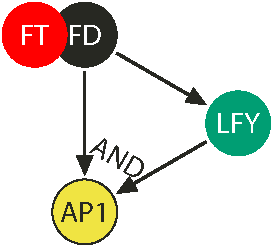
\includegraphics[width=\linewidth,page=1]{/home/nick/Dropbox/thesis/loops.pdf}
\caption{
This motif is very common in \emph{Escherichia coli}, yeast and other organisms~\cite{mangan2003}.
It has been referred to as a sign-sensitive delay element because it has a delayed on response but immediate off response~\cite{alon2006}.
}
\label{fig:cohFFL}
\end{subfigure}
\begin{subfigure}[b]{0.56\linewidth}
\includegraphics[width=\linewidth]{/home/nick/Dropbox/march2014/multinest4thesis/simpleNets/FFloopsCOH.pdf}
\caption{%Noise filtering by the coherent feedforward loop.
Responses of LFY (green) and AP1 (yellow) to a short and a long incoming FT signal (purple) are shown.
The short pulse in filtered out and the longer signal leads to (delayed) activation of AP1.
Decay in response to a fall in FT is immediate.
}
\label{fig:cohFFLdyn}
\end{subfigure}
\captionsetup{justification=centering}
\caption{The coherent feedforward loop and its dynamics.}%\label{}
\end{figure*}

The coherent feedforward loop is a network motif that is commonly found in signalling networks~\cite{mangan2003, alon2006}.
One node regulates another, with both jointly regulating a third, \autoref{fig:cohFFL}.
If the joint regulation is with an AND logic gate this simple network has persistence detection and thus is able to be used as a noise filter that removes blips in a signal.
As the correct timing of the floral transition is crucial to reproductive success it is important that the system integrates information over time, and is not incorrectly activated by noise~\cite{hasty2000}.

In the equations below we write $\theta_{FT.LFY} (FT)$ (where $\theta$ represents a Heaviside step-function) to mean that when FT is greater than (or equal to) the threshold at which it binds to the promoter site of \emph{LFY}, FT activates \emph{LFY} transcription.
Similarly $\theta_{FT.AP1} (FT)$ means \emph{AP1} is activated when FT is greater than or equal to the \emph{AP1} promoter-binding threshold.
The threshold for the activation of \emph{LFY} and \emph{AP1} is set at $\mathrm{FT}=1$.
$\theta_{LFY.AP1} (LFY)$ means that when LFY reaches a threshold, here 0.5, it binds the \emph{AP1} promoter and thus activates \emph{AP1} transcription.
The activation constants, $\nu$, and degradation constants, $\delta$, were set to 1 to scale the results to be maximally 1.
The equations for this system are therefore as follows
\begin{equation*}
\dd{LFY}{t} = \nu_{LFY} \theta_{FT.LFY} (FT) -\delta_{LFY} LFY,
\end{equation*}
\begin{equation*}
\dd{AP1}{t} = \nu_{AP1} \theta_{FT.AP1} (FT)\theta_{LFY.AP1} \left(LFY\right) -\delta_{AP1} AP1.
\end{equation*}

The dynamics of this network are shown in \autoref{fig:cohFFLdyn}.
This network motif has been described previously and has been shown to exhibit noise filtering properties for short bursts of the incoming signal that are below the delay time through the different routes in the pathway~\cite{mangan2003,alon2006}.
This is clearly seen in the figure where the short pulse of signal is filtered out whereas the longer signal is transferred through the network.
By introducing an arbitrary threshold for flowering, seen in the lower AP1 panel of \autoref{fig:cohFFLdyn}, this network shows a reversion to a non-flowering state after FT decay.

\subsubsection{The Regulated Feedforward Loop}

\begin{figure*}[!htb]
\centering
\begin{subfigure}[b]{0.42\linewidth}
\includegraphics[width=\linewidth,page=2]{/home/nick/Dropbox/thesis/loops.pdf}
\caption{
This motif is often found in developmental transcription networks~\cite{mangan2003}.
The feedback between the two targets of the first node can cause a memory effect as they keep active even in the absence of a signal from the initial regulator~\cite{alon2006}.
}
\label{fig:regFFL}
\end{subfigure}
\begin{subfigure}[b]{0.57\linewidth}
\includegraphics[width=\linewidth]{/home/nick/Dropbox/march2014/multinest4thesis/simpleNets/FFloopsREG.pdf}
\caption{%Memory created by the regulated feedforward loop.
Responses of LFY (green) and AP1 (yellow) to a short and a long incoming FT signal (purple) are shown.
The short blip leads to a small rise in LFY and AP1 levels but not enough to be maintained.
The long signal induces both targets enough so that when FT drops away the double-positive feedback loop maintains both LFY and AP1.
}
\label{fig:regFFLdyn}
\end{subfigure}
\captionsetup{justification=centering}
\caption{The regulated feedforward loop and its dynamics.}%\label{}
\end{figure*}

A similar three node network, called regulated feedforward or double-positive feedback~\cite{alon2006}, that uses an OR logic gating can exhibit irreversibility.
With the same nodes, an extra activating connection between the two targets of the first complex will mean the targets are mutually activating given enough initial impulse by the first (\autoref{fig:regFFL}).
If these conditions are met the network can provide memory of the input signal.
This is important in developmental networks because they operate on slower timescales than sensory networks.
For example commitment to flowering after exposure to long days has been shown to take 1--7 days depending on plant age and seed vernalization treatment~\cite{corbesier1996} whereas a sensory response in the shoot to salt stress in the root has been shown to take in the order of minutes, propagated in part by a rapid calcium wave~\cite{choi2014}.
%such as leaflet closure in the touch-me-not plant, \emph{Mimosa pudica}, is in the order of minutes in response to change of light conditions~\cite{burkholder1936}.
%Furthermore responses of some species to touch are well known to be in the order of seconds.
%The well studied example of the Venus fly trap, \emph{Dionaea muscipula}, shuts its trap within a second and the aforementioned \emph{M. pudica} responds to mechanical stimulation by closing its leaflets very rapidly (both reviewed by Braam~\cite{braam2005}).

The notation of the equations for this loop is identical to that for the coherent feedforward loop.
There is an additional connection in this network as shown in \autoref{fig:regFFL}.
This is controlled by the term $\theta_{AP1.LFY} (AP1)$ which means that when AP1 is greater than or equal to the threshold at which it binds to the promoter site of \emph{LFY}, AP1 activates \emph{LFY} transcription.
Both thresholds between LFY binding \emph{AP1} and vice versa were set at values of 0.45.
This creates the double-positive feedback loop~\cite{alon2006}.
Due to using OR logic gating, rather than AND logic, the equations take the higher of whichever activator is bound, leading to

\begin{equation*}
\dd{LFY}{t} = \nu_{LFY}\max\left(\theta_{FT.LFY} (FT),\theta_{AP1.LFY} (AP1)\right) - \delta_{LFY}LFY,
\end{equation*}
\begin{equation*}
\dd{AP1}{t} = \nu_{AP1}\max\left(\theta_{FT.AP1} (FT),\theta_{LFY.AP1} (LFY)\right) - \delta_{AP1}AP1.
\end{equation*}

The dynamics of this motif are shown in \autoref{fig:regFFLdyn}.
Once LFY reaches a concentration level that can activate \emph{AP1}, this interaction is sufficient to maintain AP1 production even in the absence of the incoming signal FT.
If the FT signal is removed before LFY has accumulated to a sufficient level then AP1 will degrade away before floral commitment.
The network therefore shows a memory effect and irreversibility~\cite{alon2006}.
With the arbitrary threshold for flowering, seen in the lower AP1 panel of \autoref{fig:regFFLdyn}, the double-positive feedback shows maintenance of a flowering state even after FT decay.

\subsubsection{A Compromise Feedforward Loop}

\begin{figure*}[!htb]
\centering
\begin{subfigure}[b]{0.42\linewidth}
\includegraphics[width=\linewidth, page=3]{/home/nick/Dropbox/thesis/loops.pdf}
\caption{
This network incorporates the two previous motifs by utilising different transcription rates.
A low rate requires the presence of only one signal employing an OR gate.
A higher rate of transcription can be achieved by both regulators being present so using an AND gate.
We get some noise filtering and a partial memory effect.
}
\label{fig:compFFL}
\end{subfigure}
\begin{subfigure}[b]{0.56\linewidth}
\includegraphics[width=\linewidth]{/home/nick/Dropbox/march2014/multinest4thesis/simpleNets/FFloopsCOMP.pdf}
\caption{%A compromise feedforward loop shows some noise-filtering and memory effect.
Responses of LFY (green) and AP1 (yellow) to a short and a long incoming FT signal (purple) are shown.
The blip in FT causes a damped response by both genes.
Past a threshold during the longer signal the AND gate will be switched on enabling a higher rate of transcription.
As the signal abates the transcription rate is reduced to the lower level but this is still at or above an introduced threshold for flowering.
}
\label{fig:compFFLdyn}
\end{subfigure}
\captionsetup{justification=centering}
\caption{A compromise feedforward loop and its dynamics.}%\label{}
\end{figure*}

While the previous two simple network motifs capture separate characteristics of the floral transition, in order to reproduce both noise filtering and irreversibility within the same network the logic gating rules require an extension.
This can be achieved by introducing two transcription rates, a low rate that can be activated by either FT or LFY and a higher rate that requires the presence of both FT and LFY (\autoref{fig:compFFL})
\sidenote[][-18pt]{\emph{Espinosa-Soto et al.~\cite{espinosa2004}  have used a similar idea. % in their discrete network. 
An intermediate level of expression is determined from experimental data for a number of nodes. This, as here, allows for different activation thresholds.}}%[-100pt]
.
Hence we combine the key features of both previous network motifs by using two different levels of activation depending on the number of activators bound.
The logic gating uses OR for transcriptional activation at a reduced level but requires AND for maximal activation.
The higher levels, $\nu_{LFY,1}$ and $\nu_{AP1,1}$, are set to 1, and the lower levels, $\nu_{LFY,2}$ and $\nu_{AP1,2}$, are set to 0.5.
These ideas lead to the following equations:
\begin{equation*}
\dd{LFY}{t}  =
  \begin{cases} 
\nu_{LFY,1} - \delta_{LFY}LFY & 
    \begin{aligned}[c]
       & \text{if }\theta_{FT.LFY}\left(FT\right)=1 \text{ and } \\
       & \theta_{AP1.LFY} \left(AP1\right) =1
    \end{aligned}   \\[1ex]
\!\begin{aligned}[c]
       & \nu_{LFY,2} \max\left(\theta_{FT.LFY} \left(FT\right),\theta_{AP1.LFY}
  \left(AP1\right)\right)\\
& \phantom{\nu_{LFY,1}}- \delta_{LFY}LFY
\end{aligned} & \text{otherwise,}
  \end{cases}
  \end{equation*}
\begin{equation*}
\dd{AP1}{t}  =
  \begin{cases} 
\nu_{AP1,1} - \delta_{AP1}AP1 & 
    \begin{aligned}[c]
       & \text{if }\theta_{FT.AP1}\left(FT\right)=1 \text{ and } \\
       & \theta_{LFY.AP1} \left(LFY\right) =1
    \end{aligned}   \\[1ex]
\!\begin{aligned}[c]
       & \nu_{AP1,2} \max\left(\theta_{FT.AP1} \left(FT\right),\theta_{LFY.AP1}
  \left(LFY\right)\right)\\
& \phantom{\nu_{AP1,1}}- \delta_{AP1}AP1
\end{aligned} & \text{otherwise.}
  \end{cases}
  \end{equation*}
  
This gives rise to compromised characteristics for the individual properties but it is possible to capture some level of robustness to noise and a partial memory effect.
By introducing a flowering threshold for AP1, depending on the threshold choice and parameters of the model, we can achieve irreversibility.
Thus there is sufficient memory for the system to continue to flower as shown in \autoref{fig:compFFLdyn}.

\subsubsection{Summary}

A reduced network that represents the core structure underlying the biology can be mapped to the simple feedforward loops discussed above.
As a major floral pathway integrator an active FT/FD complex was placed at the start of the transcriptional feedforward loop, upregulating another integrator, LFY, which both activate the floral initiator AP1~\cite{wagner1999}.
AP1 also mutually activates LFY in a positive feedback loop~\cite{ratcliffe1999,kaufmann2010} thus creating the important memory element which is responsible for irreversibility of a plant committed to flowering.
As this network still contains the coherent feedforward loop motif it is also able to filter out some degree of noisy endogenous or exogenous input signals, which can be relevant to a plant in its natural environment.

In this section it was sought to show a simple regulatory network that can capture two major properties of the floral transition.
This can be incorporated into a more complete model of the floral transition in Arabidopsis with our hubs and more realistic Hill-type functions from Michaelis-Menten kinetics and including the activity of the floral repressor \emph{TFL1} in a repressing hub.
This model can then be used to predict leaf numbers and generate hypotheses whilst having at its core a network that demonstrates key properties of the floral transition.

\section{Methods}

\subsection{Leaf numbers can be used to scale the network}
\label{sec:scaling}
As mentioned earlier \emph{AP1} levels have been shown to be a marker for floral commitment as \emph{AP1} is detected in early floral primordia around stages 1 and 2\cite{mandel1992,hempel1997}.
Thus in our model, the AP1 hub is chosen as the output of the floral induction pathways, and rising levels of AP1 correlate with progress through the floral transition.

\begin{figure*}[!htbp]
\centering
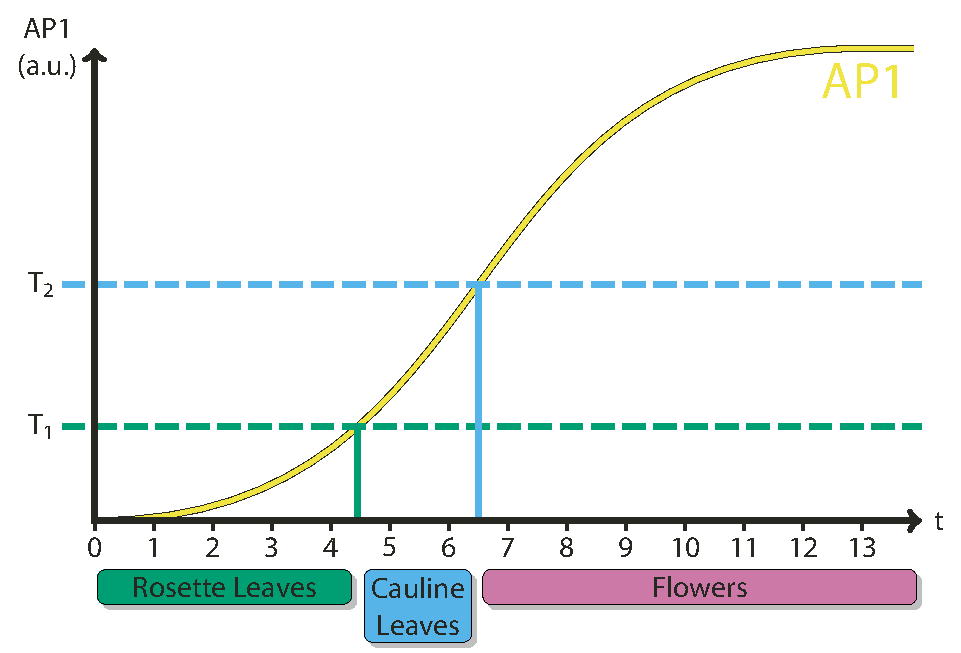
\includegraphics[width=\linewidth]{/home/nick/Dropbox/thesis/test2/sigmoid.pdf}
\caption{The definition of developmental decisions via AP1 hub levels.
An example AP1 hub curve is shown in yellow.
The developmental time taken to reach two thresholds, dashed lines, is mapped onto leaf numbers.
AP1 levels below the first threshold correspond to rosette leaves.
At the start of the transition, T\textsubscript{1}, cauline leaves are produced, and on completion of the transition, T\textsubscript{2}, flowers are made.
This mapping allows for experimental leaf number data to be used to define a cost function for inference of model parameters.
The values we used for T\textsubscript{1} and T\textsubscript{2} were 0.2 and 0.3.
a.u., arbitrary units.}
\label{fig:AP1thresholds}
\end{figure*}
After germination the first true leaves of Arabidopsis are termed rosette leaves which continue initiating during the vegetative growth phase.
We map the number of rosette leaves to the initial state and low levels of our AP1 hub.
Commencing the floral transition, lateral organs formed on the side of the bolting main shoot are termed cauline leaves.
Once the transition is complete, flowers are made.
Therefore a reliable morphological indicator of time required for initiation and length of the floral transition in the Columbia accession is the number of rosette and cauline leaves made on the main stem prior to flowers and these totals are abundantly reported throughout the literature.
To directly relate the simulated AP1 hub output to key events of the floral transition we defined two thresholds as pictured in \autoref{fig:AP1thresholds}.
The two thresholds were chosen to be at AP1 = 0.2, for the transition from rosette to cauline leaves, and at AP1 = 0.3, for the change from cauline leaves to flower production.
The decision outcome takes on one of these three states: rosette leaves, cauline leaves or flowers at these defined AP1 levels.
These threshold values are chosen arbitrarily as the parameters in the system are scaled relatively and will adjust to these selected values.
A benefit of this approach is that it can be used to quantify information on timing of both the initiation of flowering as well as the duration of the transition.
This strategy allows the developmental time to reach these states to be scaled to the leaf number data provided earlier (\autoref{tab:data}).

Having described the output of our model we now discuss the input and construction of the equations that define it.
As in the simple motifs described earlier the floral pathway integrator FT comprises a major hub for many flowering pathways.
Our model simplifies the effects of many biological and environmental processes leading to flowering by assuming they all feed in to the FT hub.
Therefore the input function to the full network model is based on FT levels.
We chose a linear time-dependent increase in FT levels until the floral transition is completed.
The transition is completed in this model when the AP1 hub threshold at 0.3 is reached and flowers are produced.
This linear with time increase of FT hub levels represents growth in leaf area proportional to time.
Further justification for this input signal is provided by the fact that the number of rosette leaves has been shown to increase at a constant rate~\cite{pouteau2009}.
The equation for the synthesis of FT is therefore $\nu_{FT}(t) = \nu_{\mathrm{FT, 35S}} + {\eta} t$, where $\eta$ is the rate of FT production per unit leaf scaled to unit time (the value chosen for this parameter was 0.01) and $\nu_{\mathrm FT, 35S}$  is the transcription rate for overexpression under the control of the 35S promoter --- if present this was taken as $1$, therefore 100 times greater than the base transcription rate in wildtype scenarios.
Genetic networks were represented by ODEs using Hill-type gene activation and repression, assuming that protein binding is in equilibrium on the timescale of translation.

\subsection{Network to Equations}

A gene network can be converted to a set of ODEs following standard practice \cite{alon2006}. 
The model includes transcriptional regulation, protein-protein interactions, and protein degradation for the hub activities in the model.
We introduce the following nomenclature.
The concentrations of the hub activity proteins are denoted by $x_1=[\mathrm{FT}]$, $x_2=[\mathrm{TFL1}]$, $x_3=[\mathrm{FD}]$, $x_4=[\mathrm{LFY}]$ and $x_5=[\mathrm{AP1}]$.
$K_{ij}$ is the effective binding constant between hub activity proteins $i$ and $j$, 
$K_{i:k}$ the effective binding constant between hub protein $i$ and a promoter site for gene $k$, 
$K_{ij:k}$ is the effective binding constant between the complex of hub activity proteins $i$ and $j$ and a promoter site for gene $k$, with $h_{i:k}$ and $h_{ij:k}$ the corresponding Hill coefficients. 
The equations governing the hub protein concentrations, $x_i$, present at any given time, $t$, are determined by the production rates, $\nu_i$, and the degradation rates, $\delta_i$, 
\begin{equation*}
\frac{dx_i}{dt}=\nu_i - \delta_{i} x_i,
\end{equation*}
in which $i=1,\ldots,5$, corresponding to FT, TFL1, FD, LFY and AP1.
The flowering time model can thus be described by differential equations, each describing the production and degradation rates for the five hubs. 
The degradation rates, $\delta_i$, were all set to a constant value, 0.1.
This can be done without loss of generality as the binding constants are allowed to change over a wide prior range to alter the effective transcription rates and adjust the effect of concentrations on downstream events. 
In reality the degradation rates are likely to differ between protein species and if the information became available these identified values can easily be substituted in to the model.

The model equations for the production rates are now discussed.
The transcription rates for the hubs are determined by the contribution from the 35S promoter, if present, $\nu_{i,\mathrm 35S}$, and a weighted sum of the rate from nothing binding to a promoter site, $\nu_{i,0}$, a singly activated level, $\nu_{i,+}$, and a doubly activated transcription rate, $\nu_{i,++}$, 
\begin{equation*}
\nu_i=\nu_{i,\rm 35S} + p_{i,0} \nu_{i,0} + p_{i,+} \nu_{i,+} + p_{i,++} \nu_{i,++}. 
\end{equation*}
The fractions, $p_i$, can be thought of as probabilities of activation and as such (including the probability of non-activation $p_{i,-}$) sum to one. 
These probabilities are determined from Hill type equations for gene activation and repression.

It is assumed that there is competitive binding between FT and TFL1 for FD~\cite{hanano2011} however this immediately complicates the equations and hence a full derivation is now given.
We assume protein-protein binding to be in equilibrium on the timescale of protein synthesis.
The total concentration of FD in the system is given by the free FD and bound FD thus $[\mathrm{FD}_{\mathrm{total}}] = [\mathrm{FD}_{\mathrm{free}}] + [\mathrm{FTFD}] + [\mathrm{TFL1FD}]$.
The concentration of FT in the system is $[\mathrm{FT}_{\mathrm{total}}] = [\mathrm{FT}_{\mathrm{free}}] + [\mathrm{FTFD}]$.
The aim is to calculate the amount of [FD] bound to [FT] and to [TFL1].
In the following we do not put square brackets, indicating concentration, or the subscripts, for clarity of presentation.
Initially, consider the concentration of FTFD and start with the assumption that free FT and FD associate at rate $k_+$ and dissociate at rate $k_-$.
Then following the law of mass-action the amount of FTFD changes over time as
\begin{equation*}
\dd{\mathrm{FTFD}}{t} = k_+\cdot \mathrm{FT}_{\mathrm{free}}\cdot \mathrm{FD}_{\mathrm{free}} - k_-\cdot \mathrm{FTFD}.
\end{equation*}
At steady state $\left(\displaystyle\dd{\mathrm{FTFD}}{t}=0\right)$ and substituting in we are left with
\begin{align*}
k_+\mathrm{FT}\left(\mathrm{FD} - \mathrm{FTFD} - \mathrm{TFL1FD}\right) &= k_-\mathrm{FTFD}, \\
\text{FTFD}\left(k_- + k_+\text{FT}\right) &= k_+\text{FT}\left(\text{FD} - \text{TFL1FD}\right),\\
\mathrm{FTFD} &= k_+\frac{\mathrm{FT}\left(\mathrm{FD} - \mathrm{TFL1FD}\right)}{k_- + k_+\cdot \mathrm{FT}}.
\end{align*}
Bringing together the binding constants in to one term, $k_d^{\mathrm{FT}}$, we are left with
\begin{equation}\label{eq:FTFDearly}
\mathrm{FTFD} = \frac{\mathrm{FT}\left(\mathrm{FD} - \mathrm{TFL1FD}\right)}{k_d^{\mathrm{FT}} + \mathrm{FT}},
\end{equation}
and by similar arguments therefore also
\begin{equation}\label{eq:TFL1FDearly}
\mathrm{TFL1FD} = \frac{\mathrm{TFL1}\left(\mathrm{FD} - \mathrm{FTFD}\right)}{k_d^{\mathrm{TFL1}} + \mathrm{TFL1}}.
\end{equation}
Substituting \eqref{eq:TFL1FDearly} into \eqref{eq:FTFDearly} as
\begin{equation*}
\mathrm{FTFD} = \frac{\mathrm{FT}}{k_d^{\mathrm{FT}} + \mathrm{FT}}\left(\mathrm{FD} - \frac{\mathrm{TFL1}\left(\mathrm{FD} - \mathrm{FTFD}\right)}{k_d^{\mathrm{TFL1}} + \mathrm{TFL1}}\right),
\end{equation*}
leaves us with
%\begin{equation}
\begin{multline*}
\left(k_d^{\mathrm{TFL1}} + \mathrm{TFL1}\right)\left(k_d^{\mathrm{FT}} + \mathrm{FT}\right)\mathrm{FTFD} = \\ \mathrm{FT}\left(\mathrm{FD}\left(k_d^{\mathrm{TFL1}} + \mathrm{TFL1}\right) - \mathrm{TFL1}\left(\mathrm{FD} - \mathrm{FTFD}\right)\right),
\end{multline*}
%\end{equation}
and after some cancelling and rearrangement
%\begin{equation}
\begin{multline*}
\left(k_d^{\mathrm{TFL1}} + \mathrm{TFL1}\right)\left(k_d^{\mathrm{FT}} + \mathrm{FT}\right)\mathrm{FTFD} - \mathrm{FT}\cdot \mathrm{TFL1}\cdot \mathrm{FTFD} = \\ k_d^{\mathrm{TFL1}}\cdot \mathrm{FT}\cdot \mathrm{FD}.
\end{multline*}
%\end{equation}
Extracting the FTFD term we are seeking and dividing across gives us
\begin{equation*}
\mathrm{FTFD} = \frac{k_d^{\mathrm{TFL1}}\cdot \mathrm{FT}\cdot \mathrm{FD}}{\left(k_d^{\mathrm{TFL1}} + \mathrm{TFL1}\right)\left(k_d^{\mathrm{FT}} + \mathrm{FT}\right) - \mathrm{FT}\cdot \mathrm{TFL1}}.
\end{equation*}
Expanding the denominator and cancelling the $FT\cdot TFL1$ term simplifies our final equation for the concentration of FT-bound FD to
\begin{equation*}
\mathrm{FTFD} = \frac{k_d^{\mathrm{TFL1}}\cdot \mathrm{FT}\cdot \mathrm{FD}}{k_d^{\mathrm{FT}}k_d^{\mathrm{TFL1}} + k_d^{\mathrm{FT}}\mathrm{TFL1} + k_d^{\mathrm{TFL1}}\mathrm{FT}}.
\end{equation*}
Analogously the equation for the concentration of FD bound to TFL1 is
\begin{equation*}
\mathrm{TFL1FD} = \frac{k_d^{\mathrm{FT}}\cdot \mathrm{TFL1}\cdot \mathrm{FD}}{k_d^{\mathrm{FT}}k_d^{\mathrm{TFL1}} + k_d^{\mathrm{FT}}\mathrm{TFL1} + k_d^{\mathrm{TFL1}}\mathrm{FT}}.
\end{equation*}
Using the previous notation
\begin{equation*}
x_{13}=x_{1}x_3 = [ \mathrm{FTFD} ]=\frac{K_{23} \cdot x_1 \cdot x_3}{K_{13}\cdot K_{23} + K_{13}\cdot x_2 + K_{23} 
\cdot x_1},
\end{equation*}
\begin{equation*}
x_{23}=x_{2}x_3 = [ \mathrm{TFL1FD} ]=\frac{K_{13} \cdot x_2 \cdot x_3}{K_{13}\cdot K_{23} + K_{13}\cdot x_2 + K_{23}
\cdot x_1}.
\end{equation*}

The transcription of \emph{TFL1} hub genes consists of a single repression rate, $\nu_{2,+}$, if one transcription factor binds and a double repression rate, $\nu_{2,++}$, with the bindings of LFY and AP1 modelled as repressing Hill functions:
\begin{equation*}
p_{5:2} = \frac{T_f^{h_{5:2}}}{T_f^{h_{5:2}}+x_5^{h_{5:2}}},
\end{equation*}
\begin{equation*}
p_{4:2} = \frac{K_{4:2}^{h_{4:2}}}{K_{4:2}^{h_{4:2}} + x_4^{h_{4:2}}},
\end{equation*}
in which $T_f$ is the threshold value of AP1 at which the plant enters the floral transition, 0.2.
Thus the transcription of \emph{TFL1} is $\nu_2 = \nu_{2, \mathrm 35S} + \nu_{2,+}\left(\left(1 - p_{5:2}\right)p_{4:2} + \left(1 - p_{4:2}\right)p_{5:2}\right) + \nu_{2,++}p_{5:2}p_{4:2} $.

As \emph{FD} is strongly upregulated during the transition~\cite{wigge2005} when floral signals such as \emph{FT} increase it is suspected it is under feedback control.
A simple explanation is that it is auto-active in this regard.
Thus the transcription of \emph{FD} hub genes consists of a base transcription rate, $\nu_{3,0}$, and an enhanced rate, $\nu_{3,+}$, when the binding of FD leads to activation.
The probability of \emph{FD} being activated through FD is
\begin{equation*}
p_{13:3} = \frac{x_{13:3}^{h_{13:3}}}
{K_{13:3}^{h_{13:3}}+x_{13}^{h_{13:3}}},
\end{equation*}
where $K_{13:3}$ is the binding constant for the FTFD complex $x_{13}$ to the promoter site of \emph{FD} ($x_3$) and $h_{13:3}$ is the corresponding Hill coefficient.
The modulator of the singly activated transcription rate of \emph{FD}, $\nu_{3,+}$, is therefore $p_{3,+}=p_{13:3}$ and the amount of base rate transcription is modulated by $p_{3,0}=1-p_{3,+}$.

The transcription of \emph{LFY} genes consists of a base transcription rate, $\nu_{4,0}$, and a singly activated rate,  $\nu_{4,+}$, when the binding of FTFD or AP1 leads to activation, and a doubly activated rate, $\nu_{4,++}$ for when both FTFD and AP1 are bound to the promoter sites of \emph{LFY}.
FTFD and TFL1FD bind competitively to one promoter site of \emph{LFY} with probabilities
%
\begin{equation*}
p_{13:4} = \frac{K_{23:4}^{h_{23:4}} \cdot x_{13}^{h_{13:4}}}
{K_{13:4}^{h_{13:4}} \cdot K_{23:4}^{h_{23:4}}+ K_{23:4}^{h_{23:4}} \cdot x_{13}^{h_{13:4}}
+ K_{13:4}^{h_{13:4}} \cdot x_{23}^{h_{23:4}}},
\end{equation*}
%
 \begin{equation*}
p_{23:4} = \frac{K_{13:4}^{h_{13:4}} \cdot x_{23}^{h_{23:4}}}
{K_{13:4}^{h_{13:4}} \cdot K_{23:4}^{h_{23:4}}+ K_{23:4}^{h_{23:4}} \cdot x_{13}^{h_{13:4}}
+ K_{13:4}^{h_{13:4}} \cdot x_{23}^{h_{23:4}}},
\end{equation*}
 %
that activate and repress the transcription, respectively. $K_{13:4}$ and $K_{23:4}$ are the binding constants for the protein complex $x_{13}$ (FTFD) and $x_{23}$ (TFL1FD) to the promoter site of the gene that codes for $x_4$ (LFY) and $h_{13:4}$ and $h_{23:4}$ are the corresponding Hill coefficients. 
AP1 also activates \emph{LFY} and this was modelled as binding to a separate promoter site (not competing with FTFD or TFL1FD), 
%
\begin{equation*}
p_{5:4} = \frac{x_{5}^{h_{5:4}}}{K_{5:4}^{h_{5:4}}+x_{5}^{h_{5:4}}}, 
\end{equation*}
%
where $K_{5:4}$ is the binding constant for the protein $x_{5}$ (AP1) to the promoter site of the gene that codes for $x_4$ (LFY) and $h_{5:4}$ is the corresponding Hill coefficient. 
Thus, for the proportion of doubly activated \emph{LFY} hub genes over time we obtain $p_{4,++} = p_{13:4} p_{5:4}$, for singly activated $p_{4,+} = p_{13:4} (1-p_{5:4}) + (1-p_{13:4} - p_{23:4}) p_{5:4}$ and for promoter sites of zero occupancy $p_{4,0} = (1-p_{13:4} - p_{23:4}) (1 - p_{5:4})$. 

Similarly the transcription of \emph{AP1} genes consists of a base transcription rate, $\nu_{5,0}$, and a singly activated rate,  $\nu_{5,+}$, when the binding of FTFD or LFY leads to activation, and a doubly activated rate, $\nu_{5,++}$ for when both FDFT and LFY are bound to the promoter sites of \emph{AP1}. FTFD and TFL1FD bind competitively to one promoter site of \emph{AP1} with probabilities 
%
\begin{equation*}
p_{13:5} = \frac{K_{23:5}^{h_{23:5}} \cdot x_{13}^{h_{13:5}}}
{K_{13:5}^{h_{13:5}} \cdot K_{23:5}^{h_{23:5}}+ K_{23:5}^{h_{23:5}} \cdot x_{13}^{h_{13:5}}
+ K_{13:5}^{h_{13:5}} \cdot x_{23}^{h_{23:5}}},
\end{equation*}
%
 \begin{equation*}
p_{23:5} = \frac{K_{13:5}^{h_{13:5}} \cdot x_{23}^{h_{23:5}}}
{K_{13:5}^{h_{13:5}} \cdot K_{23:5}^{h_{23:5}}+ K_{23:5}^{h_{23:5}} \cdot x_{13}^{h_{13:5}}
+ K_{13:5}^{h_{13:5}} \cdot x_{23}^{h_{23:5}}}. 
\end{equation*}
$K_{13:5}$ and $K_{23:5}$ are the binding constants for the protein complex $x_{13}$ (FTFD) and $x_{23}$ (TFL1FD) to the promoter site of the gene that codes for $x_5$ (AP1) and $h_{13:5}$ and $h_{23:5}$ are the corresponding Hill coefficients. 

LFY also activates \emph{AP1} hub genes and this was modelled as binding a separate promoter site (not competing with FTFD or TFL1FD), 
%
\begin{equation}
p_{4:5} = \frac{x_{4}^{h_{4:5}}}{K_{4:5}^{h_{4:5}}+x_{4}^{h_{4:5}}}, 
\end{equation}
%
in which $K_{4:5}$ is the binding constant for the protein $x_{4}$ (LFY) to the promoter site of the gene that codes for $x_5$ (AP1) and $h_{4:5}$ is the corresponding Hill coefficient. 
From this we obtain for the proportion of doubly activated LFY genes over time $p_{5,++} = p_{13:5} p_{4:5}$, for singly activated $p_{5,+} = p_{13:5} (1-p_{4:5}) + (1-p_{13:5} - p_{23:5}) p_{4:5}$, and for promoter sites of zero occupancy $p_{5,0} = (1-p_{13:5} - p_{23:5}) (1 - p_{4:5})$. 

The maximal synthesis rates are set to three values, depending on whether nothing is bound, $\nu_{i,0}$, one type of activator is present, $\nu_{i,+}$, or two types of activators are working in an AND logic activation mode, $\nu_{i,++}$. 
Production and degradation rates for the AP1 hub were chosen such that the maximal concentration is unity ($\mathrm{AP1}_{max}$ = 1) in all genotypes considered.
The complete set of equations are summarised in \autoref{tab:modelEquations}.
With no further constraints, concentrations and binding constants are not independent so we chose to vary only the binding constants and Hill coefficients in the parameter inference.
This gives a total of 19 parameters to infer.

\begin{table*}[!htbp]
\centering
\begin{tabular}{@{}l}
\toprule
Hub Protein Concentrations\\
${\displaystyle\frac{d{}x_i}{d{}t}=\nu_i - \delta_{i}  x_i}$\\
\midrule
Hub Protein-Protein Binding  \\
$x_{13} ={K_{23}  x_1  x_3}/{\left(K_{13} K_{23} + K_{13} x_2 + K_{23}  x_1\right)}$\\
$x_{23}={K_{13}  x_2  x_3}/{\left(K_{13} K_{23} + K_{13} x_2 + K_{23}  x_1\right)}$\\
\midrule
Hub Gene Activation  \\
$p_{5:2} = T_f^{h_{5:2}}/\left(T_f^{h_{5:2}}+x_5^{h_{5:2}}\right)$\\
$p_{4:2} = {K_{4:2}^{h_{4:2}}}/{\left(K_{4:2}^{h_{4:2}} + x_4^{h_{4:2}}\right)}$ \\ 
%$p_{13:2} = {K_{23:2}^{h_{23:2}}x_{13}^{h_{13:2}}} / {\left(K_{13:2}^{h_{13:2}}K_{23:2}^{h_{23:2}} + K_{23:2}^{h_{23:2}}x_{13}^{h_{23:2}} + K_{13:2}^{h_{13:2}}x_{23}^{h_{23:2}}\right)}$\\
$p_{13:3} = {x_{13}^{h_{13:3}}}/{\left(K_{13:3}^{h_{13:3}}+x_{13}^{h_{13:3}}\right)}$\\
%$p_{4:3} = {x_{4}^{h_{4:3}}}/{\left(K_{4:3}^{h_{4:3}}+x_{4}^{h_{4:3}}\right)}$\\
$p_{13:4} = {K_{23:4}^{h_{23:4}} x_{13}^{h_{13:4}}}/{\left(K_{13:4}^{h_{13:4}} K_{23:4}^{h_{23:4}}+ K_{23:4}^{h_{23:4}} x_{13}^{h_{13:4}} + K_{13:4}^{h_{13:4}} x_{23}^{h_{23:4}}\right)}$\\
$p_{23:4} = {K_{13:4}^{h_{13:4}} x_{23}^{h_{23:4}}}/{\left(K_{13:4}^{h_{13:4}} K_{23:4}^{h_{23:4}}+ K_{23:4}^{h_{23:4}} x_{13}^{h_{13:4}} + K_{13:4}^{h_{13:4}} x_{23}^{h_{23:4}}\right)}$\\
$p_{5:4} = {x_{5}^{h_{5:4}}}/{\left(K_{5:4}^{h_{5:4}}+x_{5}^{h_{5:4}}\right)}$\\
$p_{13:5} = {K_{23:5}^{h_{23:5}} x_{13}^{h_{13:5}}}/{\left(K_{13:5}^{h_{13:5}} K_{23:5}^{h_{23:5}}+ K_{23:5}^{h_{23:5}} x_{13}^{h_{13:5}} + K_{13:5}^{h_{13:5}} x_{23}^{h_{23:5}}\right)}$\\
$p_{23:5} = {K_{13:5}^{h_{13:5}} x_{23}^{h_{23:5}}}/{\left(K_{13:5}^{h_{13:5}} K_{23:5}^{h_{23:5}}+ K_{23:5}^{h_{23:5}} x_{13}^{h_{13:5}} + K_{13:5}^{h_{13:5}} x_{23}^{h_{23:5}}\right)}$\\ 
$p_{4:5} = {x_{4}^{h_{4:5}}}/{\left(K_{4:5}^{h_{4:5}}+x_{4}^{h_{4:5}}\right)}$\\
\midrule
Synthesis Rates \\
$\nu_i=\nu_{i,\mathrm 35S} + p_{i,0} \nu_{i,0} + p_{i,+} \nu_{i,+} + p_{i,++} \nu_{i,++}$\\
$p_{1,0}= 1$, $p_{1,+} = 0$, $p_{1,++} = 0$\\
$p_{2,0}= 1$, $p_{2,+} = p_{5:2}(1 - p_{4:2}) + p_{4:2}(1 - p_{5:2})$, $p_{2,++}= p_{5:2} p_{4:2}$, $T_f=0.2$\\
%$p_{3,0}=1-p_{3,+}$, $p_{3,+}=p_{4:3}$,  $p_{3,++}=0$\\
$p_{3,0}=1-p_{3,+}$, $p_{3,+}=p_{13:3}$,  $p_{3,++}=0$\\
$p_{4,0} = (1-p_{13:4} - p_{23:4}) (1 - p_{5:4})$, $p_{4,+} = p_{13:4} (1-p_{5:4}) + (1-p_{13:4} - p_{23:4}) p_{5:4}$, $p_{4,++} = p_{13:4} p_{5:4}$\\
$p_{5,0} = (1-p_{13:5} - p_{23:5}) (1 - p_{4:5})$, $p_{5,+} = p_{13:5} (1-p_{4:5}) + (1-p_{13:5} - p_{23:5}) p_{4:5}$, $p_{5,++} = p_{13:5} p_{4:5}$\\
$\nu_{1,0} = {\eta} t$, $\eta=0.01$, $\nu_{3,0} = \nu_{4,0} = 0.01$, $\nu_{2,0} = \nu_{5,0} = 0$, $\nu_{i,+}=0.05$, $\nu_{i,++} =0.1$, $\nu_{i,35S} = 1$ for $i\in\{1,\ldots,5\}$\\ 
\midrule
Initial Conditions \\
$\displaystyle\frac{\nu_{i,35S} + \nu_{i,0}}{\delta_i} $ for $i\in\{1,\ldots,5\}$\\
%$\nu_{i,35S}/\delta_i $ for $i\in\{1,2,5\}$, $\left(\nu_{i,35S} + \nu_{i,0}\right)/\delta_i $ for $i\in\{3,4\}$\\
\bottomrule
\end{tabular}
\caption{Model equations.
  The concentrations of the hub activity proteins are denoted by $x_1=[\mathrm{FT}]$, $x_2=[\mathrm{TFL1}]$, $x_3=[\mathrm{FD}]$, $x_4=[\mathrm{LFY}]$ and $x_5=[\mathrm{AP1}]$.
$K_{ij}$ are effective binding constants between hub activity proteins $i$ and $j$, 
$K_{i:k}$ the effective binding constants between hub activity protein $i$ and a promoter site for the hub activity gene $k$, $K_{ij:k}$ effective binding constants between complexes of hub activity proteins $i$ and $j$ and a promoter site for gene $k$, and $h_i$ the effective Hill coefficients.
$p_{i:k}$ is the fraction of hub activity protein $i$ bound to a promoter site of gene $k$, and $p_{ij:k}$ the fraction of the promoter of gene $k$ with the complex $i$ and $j$.
All degradation rates were set to $\delta_i=0.1$.
Initial conditions were set at $0.1$ for LFY and FD, and $0$ for the other hubs in wildtype gene scenarios.
}
\label{tab:modelEquations}
\end{table*}

\subsection{Priors for the parameters}

Uninformative priors for the parameters were chosen as we have no knowledge of their likely values \emph{in vitro} let alone \emph{in planta}.
Hill coefficients were chosen uniformly from U(1,4).
These values for Hill coefficients were also chosen in a recent DREAM challenge entry \cite{steiert2012} and are reasonable in practice \cite{sneppen2008}.
Binding coeffecients have been shown to be scale parameters \cite{grandison2008} and thus a Jeffreys-type prior was placed on those parameters with lower and upper bounds of 0.0001 and 10 respectively.

\subsection{Likelihood function}

As discussed earlier setting thresholds of the AP1 hub allows the developmental time to reach these thresholds to be scaled to leaf number data.
It is now discussed in more detail how the introduction of fixed thresholds allows for the leaf numbers to be used constructively to explore parameter space.
For all genotypes the levels of the AP1 hub are the output of our network and are mapped to the respective genotype's rosette and cauline leaf number data.
The error model was chosen to be Gaussian given the data available, \autoref{tab:data}, but as leaf numbers are integer count data a Poisson error model may be more appropriate.
The N=13 genotypes' leaf numbers in the training set are assumed to be independent with their own individual errors.
This gives a likelihood function of the form
\begin{equation*}
\mathcal L = \prod_{k=1}^N\frac{1}{\sigma_k \sqrt{2\pi}}\exp\left[\frac{-\left(f\left(\mathbf{\theta}\right)_k - \mathbf{R}_k\right)^2}{2\sigma_k^2}\right]\exp\left[\frac{-\left(f\left(\mathbf{\theta}\right)_k - \mathbf{C}_k\right)^2}{2\sigma_k^2}\right],
\end{equation*}
where $f\left(\mathbf{\theta}\right)_k$ is the function of the parameters that computes the leaf numbers. $\mathbf{R}_k$ and $\mathbf{C}_k$ are, respectively, the true rosette and cauline leaf numbers for the genotype $k$ and $\sigma_k$ the experimental standard deviation in the total leaf numbers for that genotype.
A more explicit way of writing this for our situation of evaluating the model when AP1 reaches 0.2 and 0.3, for rosette and cauline leaf numbers respectively, is the following log-likelihood function
\begin{align*}
\log\mathcal L = &-N\log\left(\sqrt{2\pi}\right) - \sum_{k=1}^N\log\sigma_k\nonumber\\ &- \sum_{k=1}^N\frac{\left(\left(\left.f\left(\mathbf{\theta}\right)_k\right|_{AP1=0.2} - \mathbf{R}_k\right)^2 + \left(\left.f\left(\mathbf{\theta}\right)_k\right|_{AP1=0.3} - \mathbf{C}_k\right)^2\right)}{2\sigma_k^2}.
\end{align*}

Having defined the data, model, prior and likelihood function we now have everything in place for a proper Bayesian treatment of the problem.
Hence the model parameters were inferred by nested sampling using the leaf number data from genotypes in the training set (wildtype, single and double mutants).
The resulting posterior distribution of the parameters for the model was used to make predictions for the triple mutants and explore the model's dynamics, sensitivity and robustness.

\section{Results}
\subsection{Biological evidence contradicts statistical evidence}

Given the data available nested sampling estimates the log evidence for the derived model to be $-56.17\pm 0.17$.
The parameters from 2000 equally-weighted posterior samples are used to give the estimated leaf numbers for all genotypes in \autoref{tab:postFDFDLeafNums}
\sidenote{\emph{Taking the parameters from the best-fit nested sample gives a maximum likelihood score of $-24.072$.
The estimated leaf numbers from this set of parameters are also given in \autoref{tab:postFDFDLeafNums}.}}
.
The network output is able to capture the true leaf numbers well for the training set and predict the triple mutant leaf numbers.
The largest predicted leaf number deviation is for the triple mutant \emph{tfl-1 fd-2 fdp-1} where the model predicts six more rosette leaves than recorded experimentally.
These inaccuracies do not surprise us.
The triple mutants were deliberately chosen as a prediction set to test the network to its fullest.
The effect of adding extra mutations is clearly not simply additive. 
The fact that our estimated leaf numbers are in the right ball park then is encouraging because we believe we have captured some of the genetic variability in our network structure.
During the undertaking of this research a paper was published \cite{winter2011} showing that FD is a target gene of LFY, at least at the seedling stage.
This could explain the observation that FD expression is strongly upregulated during the floral transition \cite{wigge2005}.
Further experiments were suggested and analysis of the FD promoter revealed it contains two LFY binding sites \cite{jaeger2013}.
It was also demonstrated that deletion of the LFY binding sites in the FD promoter abolishes FD upregulation upon the floral transition and ChIP showed that the binding was direct between LFY and the FD promoter \cite{jaeger2013}.
In light of this conclusive biological evidence we removed our hypothesised auto-activation of the FD hub which accounted for the upregulation of FD during the floral transition and replaced it with a term describing feedback from the LFY hub on to FD.
The equation for probability of FD being activated, now through LFY, becomes
\begin{equation*}
p_{4:3} = \frac{x_{4}^{h_{4:3}}}
{K_{4:3}^{h_{4:3}}+x_{4}^{h_{4:3}}},
\end{equation*}
where $K_{4:3}$ is the binding constant for LFY protein, $x_{4}$, to the promoter site of the gene that codes for $x_3$ (FD) and $h_{4:3}$ is the corresponding Hill coefficient.

\begin{table*}[!htb]
\centering
%\footnotesize
%\setlength{\tabcolsep}{3pt}
    \begin{tabular}{@{}l@{\hspace{0.8em}}ccc@{\hspace{0.5em}}c@{\hspace{1.4em}}c@{\hspace{0.7em}}c@{\hspace{0.7em}}cc@{}}
      \toprule
      Genotype  & \multicolumn{3}{c}{ No. of rosette leaves} && \multicolumn{3}{c}{ No. of cauline leaves} & Data set \\
\cmidrule(){2-4} \cmidrule(){6-8}
& True & \multicolumn{2}{c}{Model} && True & \multicolumn{2}{c}{Model} & \\
\cmidrule(){3-4} \cmidrule(){7-8}
& & Best-fit & Mean $\pm$ SD &&& Best-fit & Mean $\pm$ SD \\
%    \begin{tabular}{@{}lccccccccc@{}}
%      \toprule
%      Genotype  & \multicolumn{3}{c}{ No. of rosette leaves} && \multicolumn{3}{c}{ No. of cauline leaves} & Model set \\
%\cmidrule(r){2-4} \cmidrule{6-8}
%& Experiment & Model best-fit & Model mean $\pm$ SD && Experiment & Model best-fit & Model mean $\pm$ SD \\
      \toprule
      Wild type (Col)             & 7.9   & 8.8  &  8.7  $ \pm $  0.4  && 1.4  & 1.8  &  1.8 $ \pm $ 0.1   &  Training\\ 
      35S:\emph{FT}               & 4.4   & 4.3  &  4.1  $ \pm $  0.3  && 1.0  & 1.7  &  1.7 $ \pm $ 0.1   &  Training\\ 
      35S:\emph{LFY}              & 3.8   & 4.8  &  4.7  $ \pm $  0.1  && 1.8  & 2.1  &  2.2 $ \pm $ 0.1   &  Training\\ 
      35S:\emph{TFL1}             & 27.5  & 27.1 & 26.8  $ \pm $  1.8  && 15.7 & 15.5 & 14.4 $ \pm $ 1.9   &  Training\\ 
      \emph{lfy-12}               & 13.0  & 13.4 & 13.6  $ \pm $  0.8  && 5.3  & 4.9  &  5.1 $ \pm $ 0.4   &  Training\\ 
      \emph{ft-10}                & 36.4  & 36.7 & 37.1  $ \pm $  1.2  && 9.3  & 8.7  &  8.6 $ \pm $ 0.9   &  Training\\ 
      \emph{tfl1-1}               & 7.7   & 8.1  &  8.3  $ \pm $  0.4  && 0.4  & 1.7  &  1.8 $ \pm $ 0.1   &  Training\\ 
      \emph{fd-2}                 & 18.5  & 15.6 & 16.1  $ \pm $  1.0  && 4.63 & 3.8  &  3.7 $ \pm $ 0.3   &  Training\\ 
      \emph{fdp-1}                & 11.2  & 9.6  &  9.5  $ \pm $  0.4  && 2.0  & 1.8  &  2.0 $ \pm $ 0.1   &  Training \\
      \emph{fd-2 fdp-1}           & 32.9  & 32.1 & 31.3  $ \pm $  1.0  && 6.3  & 7.6  &  7.3 $ \pm $ 0.7   &  Training\\ 
      35S:\emph{TFL1 fd-2}        & 23.8  & 27.8 & 27.1  $ \pm $  1.9  && 8.2  & 5.2  &  5.2 $ \pm $ 0.6   &  Training \\
      \emph{tfl1-1 fd-2}          & 14.4  & 14.2 & 15.1  $ \pm $  0.8  && 4.6  & 3.7  &  3.6 $ \pm $ 0.3   &  Training \\
      35S:\emph{FT fd-2}          & 8.3   & 8.2  &  7.7  $ \pm $  0.9  && 2.4  & 2.8  &  3.0 $ \pm $ 0.4   &  Training \\
      \emph{tfl1-1 fd-2 fdp-1}    & 24.83 & 31.0 & 30.8  $ \pm $  1.1  && 6.67 & 7.5  &  7.3 $ \pm $ 0.6   &  Prediction \\
      35S:\emph{TFL1 fd-2 fdp-1}  & 31.33 & 34.2 & 34.0  $ \pm $  1.3  && 11.0 & 8.2  &  7.7 $ \pm $ 0.8   &  Prediction \\
      35S:\emph{FT fd-2 fdp-1}    & 25.8  & 26.2 & 26.3  $ \pm $  2.2  && 5.6  & 7.4  &  7.2 $ \pm $ 0.6   &  Prediction \\
      \bottomrule
    \end{tabular}
    \caption{Experimental and model leaf number data for the network with FD auto-activation.
      For each genotype the table lists the mean experimental leaf number data and estimated (for the training set) or predicted best-fit and mean $\pm$ SD values for rosette and cauline leaves.
      The best-fit values use one set of parameters and thus has no possible associated error.
      This sample is taken from all the nested samples and is the one that maximises the likelihood function the most from the final set.
      Mean and SD based on 2000 posterior samples.
      SD, standard deviation.
    }
    \label{tab:postFDFDLeafNums}
\end{table*}

Simulating this alternative network and comparing estimates of leaf number data to experimental leaf numbers reveal some differences in the training set but in sum very little.
The predictions for the triple mutants slightly favour the FD auto-regulation model but of course a full Bayesian model comparison is preferred.
Running the nested sampling algorithm with the slightly altered network architecture gave a worse log evidence score of $-62.68\pm 0.18$.
Indeed on Jeffreys' scale the Bayes factor between these two models decisively favours the original assumption that FD is an auto-activator.
How can we account for this difference between biology and statistics?
Formally the Bayes factor is only equal to the posterior odds of two models if we assume both hypotheses to be equally true.
Biologically the prior odds should favour the LFY feedback to FD model by many orders of magnitude based on the results of the experiments suggested above.
In fact given that an investigator should only define models with a reasonable verisimilitude in model space, the first hypothesis could be discounted directly.
Statistically the evidence incorporates an Occam factor \cite{mackay2003}, penalising more complex models if their fit is not substantially improved.
Comparing a basic least squares fit to the training data for the best-fitting likelihood parameters from nested sampling reveals little difference in the sum of squared errors between models, 43.1 compared to 45.7, actually in favour of the network with LFY feedback on to FD.
These numbers came from the best-fit parameter set that was found by considering the errors in the data as described by the likelihood function and then using them in a simple least-squares residual which does not consider the errors in the data.
Thus we may not want to assign much weight to this particular finding.

\begin{figure}[!htb]
\centering
% \includegraphics[height=0.35\textheight,page=6]{/home/nick/Dropbox/thesis/loops.pdf}
\includegraphics[width=0.9\textwidth,page=6]{/home/nick/Dropbox/thesis/loops.pdf}
\sidecaption[][-280pt]{New regulatory network diagram.
  This network shows all connections in the network with LFY feedback on to \emph{FD}.
  Both FT and TFL1 act through FD (small arrows) and these are shown as ovals regulating the other hubs (circles).
  FT is the input and AP1 the output of the network model.
  Filled arrowheads indicate activation and T-bars represent inhibition.
\label{fig:LFYFDdiag}}
\end{figure}

To further build an understanding of the parameter space, a simulated annealing algorithm \cite{kirkpatrick1983,goffe1994} optimising the sum of squared errors was run from a number of random starting parameter sets.
The procedure was cooled to near 0 from a starting temperature of 50, with the temperature reduction factor set at 0.85, and each exploration at a certain temperature involving 50 cycles with 20 sub-cycles.
The majority (94 out of 96 runs) of results from the initial model were near to the lowest minimum value found, 27.9.
In contrast for the new hypothesis a sole run (out of 83) was near its lowest minimum (32.0), with most (81/83) entering a wide local minima with a best fit more than double the optimal solution (around 82).
This suggests that a large amount of parameter space fits well with the FD auto-regulatory network, but not as much does with the alternative hypothesis.
This would account for a significant difference in Occam factor and can therefore help us to explain the difference in evidence results.
Ultimately the biological evidence is overwhelming for a network that has a feedback term from the LFY hub to the FD hub (depicted in \autoref{fig:LFYFDdiag}) and thus this is the model that was taken forward.

Posterior estimates of rosette and cauline leaf numbers from this newer network are shown in \autoref{fig:violinRoseCaul}.
Firstly it can be observed that we can accurately infer both types of leaf numbers with a clear idea of the uncertainty attached with those estimates or predictions.
Secondly the violin plots show (symmetrically) the distribution of our inferred leaf numbers is unimodal.
This is important because an average prediction could be the average of two, or more, predictions that are different from the experimental value.
Using a rigid methodology such as Bayesian inference allows this to be elucidated.
In this case we show that due to there being no multimodality a mean and standard deviation will give a fair summary for both the estimates and the predictions.
\begin{figure*}[!htbp]
\centering
\includegraphics[width=\linewidth]{/home/nick/Documents/multinestThesisData/LFYFD/post-leafnums/post-leaf-violin.pdf}
\caption{Estimated and predicted rosette and cauline leaf numbers for the model with LFY feedback onto FD.
2000 posterior samples were used for kernel density estimates of each genotype as a violin plot.
The x-axis positions correspond to the mean number of experimental rosette and cauline leaves.
The density estimates reveal that the predictions are unimodal.
In a perfect-fit model the violins would all be on the dark line.
}
\label{fig:violinRoseCaul}
\end{figure*}

\subsection{Dynamics of the floral transition network}

The dynamics of the wildtype network's hub proteins representing concentrations in a cell on the flanks of the apex are shown in \autoref{fig:wtDynFacet} for 2000 randomly-drawn equally-weighted posterior samples.
It can be seen that despite variability in all hubs the output hub, AP1, is under tight control.
This is not very surprising given AP1 dynamics are what constrains the likelihood function and therefore the model fitting.
FT is most variable as it approaches its steady state but in the wildtype network this has no consequence on the estimated leaf numbers.
The effect on TFL1 of being repressed is clear to see and it reaches a steady state around zero.
FD experiences the greatest delay in upregulation.
This is because it has to wait until sufficient LFY is in the system to bind and then activate it.
LFY does not accumulate immediately because there is a slight delay before the higher transcription rate is active as it needs sufficient levels of AP1 to have both promoting binding sites occupied.
AP1 transcription and translation occurs very quickly in this wildtype set-up because initial levels of LFY are present to bind to the AP1 hub promoter.
This is rapidly followed by rising FT levels which kick in to activate the higher rates of upregulation.

Throughout the time period of the floral transition strongly rising levels of the transcription factors in the network are observed.
This is in agreement with the literature~\cite{ratcliffe1998, ratcliffe1999, wigge2005}.
The behaviour of our TFL1 hub is perhaps also reflective of reality~\cite{conti2007}, at least assuming that TFL1 protein levels can be detected at a similar level to our hub levels, yet this is less clear.
Because we have modelled a cell that is poised to transition to a flower on the flanks of the apex it can be thought of as initially being in floral anlagen --- cells that form the foundations of, in this case floral, organs.
Conti \& Bradley~\cite{conti2007} show that TFL1 protein moves without its expression domain including into anlagen cells and there \emph{LFY} is expressed.
At some point these cells experience stronger floral signals and TFL1 is restricted from floral meristems.
Thus even if \emph{TFL1} mRNA is not expressed in those primordial cells at the early stages of development that this chapter focuses on, its protein product is likely to be present before declining.
This shows the early TFL1 hub dynamics in the model could be a decent description of the system.

Another point to bear in mind when critically evaluating this network's dynamics is that the input is smooth so it is not surprising that the output is smooth.
Therefore the behaviour of the network to non-monotonic input signals is investigated next along with other important dynamics representative of the floral transition to reassure ourselves that the larger network still maintains qualitative properties of the network motifs.

\begin{figure*}[!htbp]
\centering
\includegraphics[width=\linewidth]{/home/nick/Dropbox/march2014/multinest4thesis/flowering/LFYFD/post-samples/heatmap_facet_test.pdf}
\caption{2000 posterior samples of the wildtype network dynamics of the five variables.
Darker intensity indicates more samples at that concentration for each timepoint.
FT will follow the same path initially for all samples until AP1 crosses the rosette-to-cauline threshold but fans out after a while.
TFL1 is repressed as LFY and AP1 become established.
The predictive dynamics of the AP1 hub closely match each other despite the variation in the other hub proteins.
}
\label{fig:wtDynFacet}
\end{figure*}
\subsubsection{Irreversibility}
An important characteristic of the floral transition in wildtype Arabidopsis is its irreversibility.
This means that once committed to flowering the primordia can not then revert back into vegetative tissue before making floral organs.
Because FT hub mutant plants flower after a long time in suitable conditions~\cite{kim2013}, by design our network can incorporate no FT hub production term and still output flowers.
However what if there was initially FT production that was then withdrawn?
This could represent for instance a light shift experiment from long days to darkness or a construct that can inducibly knockdown FT.
This was investigated by setting the FT production term, $\nu_{FT}$, in the model to zero after a certain number of leaves had been observed.
Simulations, using the best-fit parameters, varying the length of inductive conditions are shown in \autoref{fig:irrev}.
\begin{figure*}[!htb]
\centering
\includegraphics[width=\linewidth]{/home/nick/Dropbox/march2014/multinest4thesis/flowering/figures/irrev.pdf}
\caption{The effect of FT production withdrawal on the AP1 hub.
FT is withdrawn after the indicated number of leaves and its effect on the correspondingly coloured lines for AP1 is shown.
Flowering time is judged by AP1 crossing the 0.3 threshold.
Longer times equate to delayed flowering.
The wildtype (WT) and FT-knockout (ft) scenarios are shown for comparison.
Even a small induction of FT speeds up the time to flower compared to the knockout line.
}
\label{fig:irrev}
\end{figure*}
Flowering time is judged here by AP1 crossing the 0.3 threshold.
As can be seen flowering time is identical to the wildtype if FT is stopped after a developmental time of 10 leaves, and near identical if terminated at the eight leaf stage.
Ceasing FT production after the formation of six leaves causes a slightly delayed time to flower.
On the other hand the duration of FT production has a strong effect on the timing of flowering if withdrawn early, at the two or four leaf stage.
Compared with the simulated complete lack of the FT hub (labelled ft in \autoref{fig:irrev}) flowering is still accelerated when FT production is withdrawn after the formation of only two leaves.
Once AP1 has crossed the rosette-to-cauline threshold (0.2; around the 8 leaf stage) preventing FT production has little effect on the timing of flowering.
At this point the plant is committed to flowering which is consistent with a study showing that one long day can be sufficient to cause floral commitment under certain conditions~\cite{corbesier1996}.
Thus by introducing a flowering threshold this network can exhibit irreversibility, and from earlier we know this is due to the memory element present in the core regulatory motif.

\subsubsection{Noise Filtering}

\emph{FT} expression is strongly influenced by temperature~\cite{balasubramanian2006}.
Therefore plants are likely to experience large day-to-day fluctuations in \emph{FT} levels.
To simulate these conditions first uniform random noise of up to 50\% of the signal $\nu_{FT}$ was given as input.
With this level of noise FT hub levels are only minorly perturbed, \autoref{fig:noisy} Left, with no effect on the AP1 hub.
Pushing this further very high noise levels in FT production rates were simulated such that uniform random noise of up to 200\% $\nu_{FT}$ was given as input.
These signals propagate through to the levels of FT, \autoref{fig:noisy} Right, however the network is also able to filter this out, resulting in a smooth AP1 curve.
Under these conditions the model simulates the ability of this developmental system to filter noisy environmental signals and make correctly timed decisions.
The buffering properties of the model result in AP1 levels that are unaffected by these perturbations because of the incorporated coherent feedforward loop.
\begin{figure*}[!htb]
\centering
\includegraphics[width=\linewidth]{/home/nick/Dropbox/march2014/multinest4thesis/flowering/figures/noisy.pdf}
\caption{Effect of signal noise on the network hubs.
50\% (left) or 200\% (right) random noise was added to the signal (purple).
The lower level of noise in the FT input barely filters through to the FT hub (red) thus not surprisingly the AP1 (yellow) output is smooth.
The high noise levels affect the FT hub more strongly but they are also filtered out by the network so there is no effect on the AP1 hub.
}
\label{fig:noisy}
\end{figure*}

\subsubsection{Circadian Oscillations}
Both FT hub genes \emph{FT} and \emph{TSF} are expressed in a circadian fashion \emph{in planta}~\cite{suarezlopez2001,yamaguchi2005}.
\emph{AP1} expression, our marker for the output of the flowering pathway, does not oscillate~\cite{sundstrom2006}.
We wished to test how well our full regulatory network also exhibits this ability to integrate out and smooth input signals.
Hence it was examined how oscillating production rates of FT influence the FT and AP1 hubs in particular.
The input term, $\nu_{FT}$, was multiplied by the oscillating function $\sin(ct)^2$, where c controls the frequency, either 0.5 (\autoref{fig:circ} Left) or 3 (\autoref{fig:circ} Right).
As shown in these figures the network is able to filter out large oscillations in FT production rate at both high and low frequencies.
These modulations propagate through to FT levels yet generate an unperturbed increase in AP1.

\begin{figure*}[!htbp]
\centering
\includegraphics[width=\linewidth]{/home/nick/Dropbox/march2014/multinest4thesis/flowering/figures/circ.pdf}
\caption{Effect of oscillating FT input signal on the network hubs.
Upper row: degradation rates are set at 0.1 as used throughout this chapter.
The circadian oscillations at low frequency (left) of FT activation (purple) propagate through to the FT hub (red) with no effect on the AP1 hub (yellow).
High frequency (right) FT activation oscillations transmit through to the FT hub with small amplitude and thus this does not prevent a smooth rise in the AP1 hub.
Lower row: the degradation rates are doubled to 0.2.
Very small modulations are seen at the start of the AP1 hub curve due to the massive amplitude in the FT hub's oscillations (left).
High degradation rates and fast oscillating FT input signal again damp the FT hub's dynamics without affecting AP1 (right).
}
\label{fig:circ}
\end{figure*}

As stated previously our proposed network contains a motif that is known to buffer noise well.
However in this flowering time model the ability to buffer noise is also partly a result of the magnitude of the degradation rates compared to the steady state values.
Doubling the degradation rates, such that the modulation in $\nu_{FT}$ is fed through even more strongly to FT, we still find that the network filters out these perturbations, \autoref{fig:circ} (Lower row).
The full model therefore captures key properties of the floral transition in Arabidopsis, including irreversibility and the filtering of noisy and circadian signals, due to the network motifs built into its architecture.

\subsection{Parameter analysis}

The marginal distributions of the 19 parameters over their prior range are shown in \autoref{fig:flowerMarg}, and then after zooming in on regions of non-zero probability in \autoref{fig:flowerMargZoom}.
These distributions show a number of interesting things justifying the use of a Bayesian treatment of the problem.
We note how some Hill parameters can take on most values of their prior and thus are not constrained by the data.
In constrast the data constrains some parameters very strongly.
As these distributions are correctly normalised to have an area equalling one the parameters with higher values are the ones that are most defined.
In particular the binding coefficient of LFY on to the \emph{TFL1} promoter, $K_{4:2}$, has a high probability in the region between $10^{-4}$ and $10^{-2}$.
The parameters controlling the binding coefficient of a number of species to \emph{AP1} are also well defined.
This perhaps does not surprise because the AP1 levels are the output of our system and must therefore be constrained to give a reasonable likelihood score.
No parameters seem to show multimodality in their marginal distributions, but not all have one strong peak.
This discovery might not be accounted for with classical statistical techniques.
For example the mean and standard deviation of the Hill parameter controlling the binding of the TFL1FD hub complex to \emph{AP1}, $h_{23:5}$, would completely miss the fact that more weight is given to the higher end of the parameter value, around 4. 

In fact this case highlights a strength of the Bayesian approach as it can raise a concern, leading one to investigate model reliability but providing an avenue for updating our degrees of belief.
It seems that high Hill coefficients are preferred for both $h_{23:5}$ and $h_{4:3}$, meaning that for a second round of inference maybe the prior range should be extended.
However such large Hill terms are improbable in many realistic situations.
To account for this habit of large Hill coefficients resulting from parameter inference we could either be more specific with our prior belief on the parameters by choosing a different prior distribution, or one could add a penalty to the likelihood function.
A simple prior distribution to consider here could be a triangular distribution with most weight at the end nearest one and little weight at high values of the Hill parameter.
If the data were not informative enough to overcome our prior belief then the parameters' posterior distribution would be dominated by the prior thus alleviating the problematic high Hill coefficients.
In this flowering time model uniform priors were initially chosen for all Hill parameters as we had no knowledge of their likely values.
After examining the posterior we have revealed that firstly, if the analysis was updated then two parameters ought to have different prior distributions, and secondly that our data does not constrain the choice of all parameters to realistic values.

\begin{figure*}[!htbp]
\centering
\includegraphics[width=\linewidth]{/home/nick/Dropbox/march2014/multinest4thesis/flowering/LFYFD/margAndJoints/marginalsBasic.pdf}
\caption{Estimated marginal posterior parameter distributions over prior range.
The kinetic parameters, $K_*$, have a $\log_{10}$-uniform prior range of $[10^{-4},10]$.
The Hill terms, $h_*$, follow the prior $U(1,4)$.
More kinetic parameters than Hill parameters have a higher probability density indicating they are the more constrained.
All marginals have been properly normalised with area equal to one, thus the y-axis values represent estimated probability densities.
}
\label{fig:flowerMarg}
\end{figure*}
\begin{figure*}
\includegraphics[width=\linewidth]{/home/nick/Dropbox/march2014/multinest4thesis/flowering/LFYFD/margAndJoints/marginalsZoom.pdf}
\caption{Estimated marginal posterior parameter distributions zoomed in on non-zero probability regions.
No parameters are multimodal however not all have one strong mode.
Some Hill parameters can take on most prior values with almost equal probability.
Intriguingly this applies for $h_{4:2}$ which is the Hill term for binding of LFY on to the \emph{TFL1} promoter whereas its corresponding kinetic parameter ($K_{4:2}$) is the mostly tightly controlled parameter.
Y-axis values represent estimated probability densities with marginal distribution area equal to one.
}
\label{fig:flowerMargZoom}
\end{figure*}

\begin{figure*}[!htbp]
  \centering
  \includegraphics[width=\linewidth]{/home/nick/Dropbox/march2014/multinest4thesis/flowering/LFYFD/margAndJoints/jointsZoomRandom.pdf}
  \caption{Estimated joint posterior parameter distributions for selected parameters.
    A sample of joint distributions of different parameter values gives a better understanding of parameter space.
    Brighter colours indicate higher relative probability.
    % Top row: Parameters 0 and 1; Parameters 3 and 7.
    % Middle row: Parameters 4 and 5; Parameters 8 and 12.
    % Bottom row: Parameters 10 and 15; Parameters 16 and 18.
  }
  \label{fig:flowJointRan}
\end{figure*}
\begin{figure*}[!htbp]
  \centering
  \includegraphics[width=\linewidth]{/home/nick/Dropbox/march2014/multinest4thesis/flowering/LFYFD/margAndJoints/jointsZoomCorrelated.pdf}
  \caption{Estimated joint posterior parameter distributions showing correlations.
    All joint distributions were studied and the ones presented here show the most interesting correlations between parameters.
    Joint distributions can reveal hard to uncover information about parameter space such as correlations or multimodality.
    Brighter colours indicate higher relative probability.
    % Top row: Parameters 0 and 6; Parameters 1 and 4.
    % Middle row: Parameters 1 and 7; Parameters 1 and 8.
    % Bottom row: Parameters 2 and 5; Parameters 7 and 8.
  }
  \label{fig:flowJointCorr}
\end{figure*}

A selection of joint distributions between parameters is shown in \autoref{fig:flowJointRan}.
No combinations of parameters appear multimodal although there are correlations in some combinations (\autoref{fig:flowJointCorr}).
For example, $K_{4:3}$, the parameter controlling the binding of LFY onto \emph{FD} exhibits some correlation with other parameters.
The binding constants of the two mutual activators, \emph{AP1} and \emph{LFY}, to each other show a surprising yet evident non-linear correlation (\autoref{fig:flowJointCorr} Bottom right).
Some parameter joint distributions are so spread out that they essentially look uniformly randomly distributed as in \autoref{fig:flowJointRan} (Bottom row).
These interesting figures all together show that evaluating the posterior distribution will enable one to find more information, such as the spread or correlations, that can be missed from a point estimate of the parameters.
Likewise it can be inferred that some parameters are far more sensitive to their choice than others, and thus in the future this could be an avenue for minimising the proposed model.

Additionally the effect of some parameters on the flowering time of the wildtype network was investigated qualitatively.
It was found that the interplay between $K_{13}$ and $K_{23}$ was very important.
This is intuitive as these parameters control the relative binding strength of FD to either FT or TFL1.
Tighter TFL1 binding to FD leads to delayed flowering, which can be compensated for by lowering $K_{13}$ even more, to give tighter binding between FT and FD.
The competition for FD binding is therefore critical to correct flowering time for the input but what about for the output?
Reducing values of $K_{23:5}$, controlling the binding of the TFL1FD complex on to the \emph{AP1} promoter, again leads to a delay in AP1 accumulation.
As previously this effect can be counterbalanced by decreasing the value of $K_{13:5}$ so that FTFD binds more tightly to the \emph{AP1} promoter.

Satisfyingly these results support a number of experimental studies.
The proposal that FT may interact with FD amongst others in a transcriptional complex more strongly than TFL1 to activate flowering genes~\cite{hanano2011} is endorsed by the qualitative analysis of our network.
Yeast two-hybrid assays have shown that FT interacts more strongly with FD than TFL1 in yeast~\cite{abe2005,hanano2011}.
Looking at the marginal distributions in \autoref{fig:flowerMargZoom} of the parameters controlling the same interactions, $K_{13}$ and $K_{23}$, shows that the values for $K_{23}$ are higher leading to its weaker binding to FD in our model.
These results increase the belief that the model really captures some of the biology with how the network was constructed and the statistical treatment of the problem of parameter inference.

\subsection{A hint on spatial patterning of the SAM?}

Having established a network architecture that captures the temporal dynamics of cells undergoing the floral transition we also tentatively wondered if the model might also help us understand the spatial expression patterns of the main floral meristem regulators.
This is a particularly interesting question because during development plants show sharp boundaries of gene expression in the SAM.
During the floral transition initially diffuse and variable input signals, for example FT, gradually increase over time, leading to the expression of floral meristem genes such as \emph{LFY} and \emph{AP1} on the flanks of the shoot, while the centre of the shoot has rising \emph{TFL1} expression and remains vegetative.
It was hypothesised that low initial levels of the LFY or TFL1 hubs in the model might be sufficient to determine the stable acquisition of either a flowering (high AP1) or vegetative (high TFL1) state.
Switching between these initial conditions the wildtype network has not been found to exhibit a bistable outcome between flowering or vegetative fates.
Instead, a flowering state is often reached depending on the parameters (as discussed above).

This is expected for a number of reasons.
As the temporal model has flowers as its output, as mentioned, it can be thought of as representing a cell on the flanks of the shoot apex poised to transition.
These cells transition to a high AP1 state, but they do not experience extended upregulation of TFL1, since \emph{TFL1} is repressed in floral meristems~\cite{ratcliffe1999}.
By contrast, within the centre of the shoot, \emph{TFL1} is strongly upregulated upon flowering.
\begin{marginfigure}
    \includegraphics[width=\marginparwidth]{/home/nick/Dropbox/sept2013/PLOS1REVISIONS/tanh-FT-TFL1-plot/thesis-FT-TFL1.pdf}
    \caption{Reproduction of \autoref{fig:FT-TFL1-data}.
      There is a clear positive relationship between \emph{TFL1} and \emph{FT} expression levels as determined by qPCR.
  }
  \label{fig:FT-TFL1-data-FTchap}
\end{marginfigure}
It was found after experimental discussions that \emph{TFL1} expression correlates across an entire Arabidopsis plant with the level of \emph{FT} expression as shown in \autoref{fig:FT-TFL1-data-FTchap} (exactly the same as \autoref{fig:FT-TFL1-data} in the previous chapter).
The simplest way of accounting for this behaviour in our model was to include a term for the activation of \emph{TFL1} by FTFD in the network, as shown in \autoref{fig:FTFDTFL1diag}.
\begin{marginfigure}%[!htb]
%\centering
\includegraphics[width=\marginparwidth,page=7]{/home/nick/Dropbox/thesis/loops.pdf}
%\includegraphics[width=0.9\textwidth,page=7]{/home/nick/Dropbox/thesis/loops.pdf}
%\sidecaption[][]{Enhanced regulatory network diagram.
\caption{Enhanced regulatory network diagram.  
  This network shows an additional connection between FTFD and TFL1.
  Filled arrowheads indicate activation and T-bars represent inhibition.
\label{fig:FTFDTFL1diag}}
\end{marginfigure}
Given our hub structure this need not be a direct interaction, indeed it surely involves a number of intermediaries \emph{in planta}.
In \autoref{chapter:nestedSampling} it was seen that for this data a sigmoidal model had a strong weight of evidence for it against a linear model.
This suggests we can justifiably keep the similar structure based on Hill equations in terms of hub binding for this interaction.
The addition of this connection requires four extra parameters for FTFD binding to the promoter of \emph{TFL1} as described by the following equation
\begin{equation*}
p_{13:2} = \frac{K_{23:2}^{h_{23:2}}x_{13}^{h_{13:2}}}{K_{13:2}^{h_{13:2}}K_{23:2}^{h_{23:2}}
+ K_{23:2}^{h_{23:2}}x_{13}^{h_{23:2}} + K_{13:2}^{h_{13:2}}x_{23}^{h_{23:2}}}.
\end{equation*}

To avoid complicating the model even further this term was simply multiplied by the doubly activated TFL1 rate which leads to a competition between activation through FTFD and repression from AP1 and LFY.
Hence when AP1 and LFY are present at high concentration they will be dominantly repressive over the effect of direct FTFD-induced transcription of TFL1.
The new term for TFL1 activation is then
\begin{equation*}
\begin{split}
\nu_2 = \ &\nu_{\mathrm TFL1, 35S} \\ +\ & \nu_{TFL1,+}((1 - p_{5:2})p_{4:2} + (1 - p_{4:2})p_{5:2}) \\ +\ & \nu_{TFL1,++}\cdot p_{5:2}\cdot p_{4:2}\cdot p_{13:2}.
\end{split}
\end{equation*}

\begin{table*}[!htb]
  \centering
  % \footnotesize
  \setlength{\tabcolsep}{5pt}
  \begin{tabular}{@{}l@{\hspace{0.8em}}ccc@{\hspace{0.5em}}c@{\hspace{1.4em}}c@{\hspace{0.7em}}c@{\hspace{0.7em}}cc@{}}
    \toprule
    Genotype  & \multicolumn{3}{c}{ No. of rosette leaves} && \multicolumn{3}{c}{ No. of cauline leaves} & Data set \\
    \cmidrule(){2-4} \cmidrule(){6-8}
    & True & \multicolumn{2}{c}{Model} && True & \multicolumn{2}{c}{Model} & \\
    \cmidrule(){3-4} \cmidrule(){7-8}
    & & Best-fit & Mean $\pm$ SD &&& Best-fit & Mean $\pm$ SD \\
    \toprule
      Wild type (Col)             &  7.9  & 8.9  &  8.7 $ \pm $ 0.4 &&  1.4  & 2.0 &  1.9  $ \pm $  0.09 & Training\\
      35S:\emph{FT}               &  4.4  & 3.6  &  3.8 $ \pm $ 0.2 &&  1.0  & 1.6 &  1.7  $ \pm $  0.06 & Training\\
      35S:\emph{LFY}              &  3.8  & 3.9  &  4.1 $ \pm $ 0.1 &&  1.8  & 1.5 &  1.6  $ \pm $  0.04 & Training\\
      35S:\emph{TFL1}             & 27.5  & 26.8 & 28.1 $ \pm $ 1.5 && 15.7  & 16.9& 14.3  $ \pm $  1.9 & Training\\
      \emph{lfy-12}               & 13.0  & 12.3 & 12.8 $ \pm $ 0.7 &&  5.3  & 6.2 &  6.6  $ \pm $  0.6 & Training\\
      \emph{ft-10}                & 36.4  & 35.5 & 37.0 $ \pm $ 1.4 &&  9.3  & 8.6 &  8.8  $ \pm $  1.0 & Training\\
      \emph{tfl1-1}               &  7.7  & 8.3  &  8.5 $ \pm $ 0.4 &&  0.4  & 1.9 &  1.9  $ \pm $  0.08 & Training\\
      \emph{fd-2}                 & 18.5  & 18.1 & 16.1 $ \pm $ 0.8 &&  4.63 & 3.9 &  3.4  $ \pm $  0.3 & Training\\
      \emph{fdp-1}                & 11.2  & 9.8  &  9.4 $ \pm $ 0.4 &&  2.0  & 2.2 &  2.1  $ \pm $  0.1 & Training\\
      \emph{fd-2 fdp-1}           & 32.9  & 32.8 & 31.6 $ \pm $ 0.9 &&  6.3  & 7.0 &  6.8  $ \pm $  0.6 & Training\\
      35S:\emph{TFL1 fd-2}        & 23.8  & 25.3 & 26.0 $ \pm $ 1.5 &&  8.2  & 4.5 &  4.5  $ \pm $  0.4 & Training\\
      \emph{tfl1-1 fd-2}          & 14.4  & 15.4 & 15.6 $ \pm $ 0.7 &&  4.6  & 3.4 &  3.3  $ \pm $  0.3 & Training\\
      35S:\emph{FT fd-2}          &  8.3  & 8.3  &  7.0 $ \pm $ 0.8 &&  2.4  & 3.4 &  2.8  $ \pm $  0.3 & Training\\
      \emph{tfl1-1 fd-2 fdp-1}    & 24.83 & 30.2 & 31.2 $ \pm $ 1.0 &&  6.67 & 6.6 &  6.7  $ \pm $  0.6 & Prediction\\
      35S:\emph{TFL1 fd-2 fdp-1}  & 31.33 & 34.0 & 34.9 $ \pm $ 1.1 && 11.0  & 7.2 &  7.3  $ \pm $  0.7 & Prediction\\
      35S:\emph{FT fd-2 fdp-1}    & 25.8  & 28.5 & 26.1 $ \pm $ 2.1 &&  5.6  & 6.8 &  6.6  $ \pm $  0.6 & Prediction\\ 
      \bottomrule
    \end{tabular}
    \caption{Experimental and model leaf number data for the extended network with FTFD activating TFL1.
      For each genotype the table lists the mean experimental leaf number data and estimated (for the training set) or predicted best-fit and mean $\pm$ SD values for rosette and cauline leaves.
      The best-fit values use one set of parameters and thus have no possible associated error.
      This sample is taken from all the nested samples and is the one that maximises the likelihood function the most from the final set.
      Mean and SD based on 2000 posterior samples.
      SD, standard deviation.
      \label{tab:postExtLeafNums}
      }
\end{table*}

It was tested whether this network was still capable of fitting to the leaf numbers and if so, how its Bayesian evidence ranked compared to the two models previously considered.
Running nested sampling on the same data set but with this extra connection in the model gave a log evidence of $-59.87\pm 0.18$.
The previous model, with LFY feedback on to \emph{FD}, had a log evidence of $-62.68\pm 0.18$ thus the Bayes factor is just under $3$ --- and on a normal scale is favoured $16:1$.
On Jeffreys' scale this would be strong evidence in favour of a model with this extra term despite the four additional parameters.
What is the basis for this improvement in evidence?
It is known (see \autoref{ssec:BayesModComp} and also MacKay~\cite{mackay2003}) the evidence comprises an Occam factor and a measure of goodness of fit.
Here the former should penalise our extended model requiring four more parameters, and the latter should give more accurate leaf number estimates.
Intriguingly much of the improvements come through superior estimates of mutations solely affecting the FD hub \autoref{tab:postExtLeafNums}.
The genotypes \emph{fd-2}, \emph{fdp-1} and \emph{fd-2 fdp-1} all have better estimated best-fits in the extended model, in particular the rosette leaves of the \emph{fd} mutant.
In the training set for all three network models the best-fit leaf number estimates of genotype \emph{35S:TFL1 fd-2} are the source of the poorest fits.
This suggests we haven't done as well capturing the suppression of \emph{35S:TFL1} by \emph{fd-2} as other genotypes.
In terms of predicting the triple mutant leaf numbers there are no substantial improvements or regressions.

For different parameter values, the vegetative centre of the SAM was simulated, where \emph{TFL1} is initially expressed at low levels and \emph{LFY} is absent~\cite{bradley1997,ratcliffe1998,ratcliffe1999}.
In this model scenario, rising levels of FT trigger the further upregulation of \emph{TFL1}.
The negative feedback of TFL1 onto both \emph{AP1} and \emph{LFY} prevents their expression (\autoref{fig:spatPAT} Top).
Under the opposite starting conditions, low levels of LFY and no initial TFL1, corresponding to the primordium prior to floral evocation, rising FT activates AP1 and LFY.
Since this is a positive feedback loop, high levels of AP1 and LFY are rapidly established, and TFL1 is repressed, leading to a floral state (\autoref{fig:spatPAT} Bottom).
Although no parameter sets have been found where this is a stable state --- at very high leaf numbers (when in practice the plant may have already died) this breaks down and AP1 reaches the flowering threshold --- this can be seen as a starting hypothesis that warrants future investigations.
Up until late developmental times essentially the winner takes all --- vegetative or flowering programs are established --- depending on the initial levels of either TFL1 or LFY and their sharp rise through the transition.
This simulated outcome supports the model of Ratcliffe et al.~\cite{ratcliffe1999} who suggest that one possibility for the spatial patterning is due to the relative timing of \emph{TFL1} and the floral genes' induction, and subsequent mutual inhibition in the centre or periphery of the apex.
In addition this gives us a lead to understanding the spatial patterning of the SAM where the activators of the transition must also cause a synchronous activation of their own repression in certain domains presumably due to floral signals being perceived by upstream regulators of meristem identity.
This patterning mechanism has parallels with floral induction in tomato, where the floral signal SFT upregulates a repressor of floral meristem fate in lateral meristems adjacent to floral meristems~\cite{thouet2012}.
Further understanding the system of apical patterning is an exciting goal for researchers in the future.

\begin{figure}[!htb]
\centering
% \includegraphics[height=0.35\textheight,page=6]{/home/nick/Dropbox/thesis/loops.pdf}
\includegraphics[width=\textwidth]{/home/nick/Dropbox/march2014/multinest4thesis/flowering/FTFDTFL1/spatPAT/LFY-TFL1-spat.pdf}
\sidecaption[][-300pt]{Initial conditions can determine apical cell state.
  For the timepoints shown a switch between initial conditions of LFY (green solid line) and TFL1 (blue dash-dot line) affect hub behaviour.
  Top: LFY starts at 0, TFL1 at 0.1. TFL1 is able to repress LFY and AP1 due to continued increase in FT levels.
  Bottom: Under opposite starting conditions where LFY is initially 0.1 and TFL1 is 0, LFY and AP1 are increased and flower normally while TFL1 is repressed.
\label{fig:spatPAT}}
\end{figure}

\section{Discussion}

\subsection{Strengths and limitations of the model}

A challenge to modelling complex biological systems, such as the floral transition, is that many interacting components are involved and little is known in terms of their biophysical properties such as biochemical concentrations, binding affinities for each other or half lives within the cell.
The mathematical modelling presented here thus involves considerable simplifications in terms of quantitative cell biology.
We also simplified much hard work from excellent genetic studies in Arabidopsis with the reductionist approach --- using knowledge of the major components and approximating key genes for entire hub activities.
The list of things approximated and not modelled explicitly is vast.
Therefore it is worth providing a brief list where more details are available in \autoref{sec:ftGenetics}.
In Arabidopsis a number of pathways~\cite{simpson2002,srikanth2011} converge to stimulate flowering.
This chapter focused on FT, a key floral integrator, as the input to the network.
In one fell swoop this approximated the photoperiod pathway, whose output is diurnal \emph{FT} expression; the vernalisation pathway\sidenote{\emph{Although the rapid-cycling wildtype Columbia-0 accession used as the genetic background for the genotypes in this thesis does not have this requirement.}}; and the autonomous pathway.
The age-dependent and gibberellin pathways were accounted for by gradually rising levels of the AP1 and LFY hubs.
Numerous other players in this web have been implicated: SPL transcription factors~\cite{wang2009,yamaguchi2009}, the floral integrator gene SOC1~\cite{liu2008}, hormones such as auxin~\cite{yamaguchi2013} and cytokinin~\cite{daloia2011}, various microRNAs~\cite{schmid2003}, ambient temperature~\cite{blazquez2003,kumar2012, balasubramanian2006} and the role of mechanical forces~\cite{hamant2008}.

The model was motivated by known biological interactions and the idea of using the available leaf number data to make the predictions quantitative.
This allowed us to train the network to the data and enabled the resulting model to suggest experiments that can be related back to biological entities.
We did this by defining two thresholds at effectively arbitrary values of 0.2 and 0.3.
Given the number of parameters in the model it is reasonable to believe that sensibly changing the values of these thresholds would just lead to a corresponding altering of the parameter distributions such that we still fit to the data at a similar level.
The network model is also simple enough to understand some aspects of it intuitively because of the well-studied motifs it is based on.
These advantages comes at a cost.
First, by placing the network in an ordinary differential equation framework, we need to carry out computationally costly parameter space sampling.
Although the employed nested sampling routine has been shown to perform very well for this purpose it is still true that we do not know whether or not our estimated parameter distributions are realistic or not.
Second, the reduction to activity hubs means that our individual genes do not have direct \emph{in planta} equivalents.
Despite basing our equations on kinetic binding between proteins these are actually ``hub proteins'' and therefore an approximation of the effects of different proteins in the plant.
Third, the model currently largely neglects important spatial effects.
Although we can reproduce the overall behaviour of the transition, individual interactions represent spatially averaged behaviour and conclusions from this simplified network about such details must be considered carefully.
For example we defined an appropriate network that represents well a single cell in the apex periphery that is capable of entering the transition.
A cell elsewhere in the apex may, in fact, have a different set of connections between hubs and thus experience somewhat different behaviour.

Linear modelling of the system as presented in the early part of this chapter also suffers from these limitations, and more besides.
The network approach taken here performs better than the linear model because it helps us to understand and explain dynamic behaviour.
The increase in parameters this required also gives us more flexibility in the fitting to the leaf number data.
Thus we are able to be more accurate in estimating the training genotypes along with predictions that more closely match the triple mutant data --- along with the individual rosette and cauline leaf data shown above compare \autoref{fig:TotalLeafViolin} with \autoref{fig:FTlinearIndSig} or \autoref{fig:FTlinear}.
It is also worth noting that all the network models had decisive evidence for them versus the linear model as judged on Jeffreys' scale.

\begin{figure*}[!htbp]
\centering
\includegraphics[width=\linewidth]{/home/nick/Dropbox/march2014/multinest4thesis/flowering/TOTALleafnums/post-leafnums/post-TOTAL-leaf-violin.pdf}
\caption{Posterior sampling of the extended model for total leaf numbers.
Nested sampling was run with a likelihood function that minimised the sum of the model rosette and cauline leaves against the true total leaf number.
2000 posterior samples were taken and summary statistics calculated for each genotype.
Compared with the linear models' summaries, \autoref{fig:FTlinearIndSig} and \autoref{fig:FTlinear}, these estimates and predictions are far more reflective of the real data.
We don't predict \emph{35S:TFL1 fd-2 fdp-1} as accurately as in the linear model but we are now more accurate for the entire data set.
The evidence for this model, $-47.96\pm 0.15$, is far better than the linear models' thus showing that, for this data set, the increase in parameters is quantitatively justifiable and that the network approach is considerably more powerful than linear modelling.
}
\label{fig:TotalLeafViolin}
\end{figure*}

Our model is also extensible.
Adding further hubs to this network, for example SOC1, is not too difficult and will lead to further testable hypotheses.
More expansively, models for the circadian clock~\cite{song2012} upstream of the floral transition as well as models for downstream processes such as MADS-box transcription factors specifying floral organs~\cite{vanmourik2010} could in theory all be coupled together to produce a more complete picture of floral morphogenesis at the SAM.

\subsection{Outlook}

Due to the clear mathematical foundations and robust statistical treatment of our modelling there are a number of directions this work could be expanded on in the future.
In Arabidopsis two clear paths present a fork in the road depending on what one is trying to achieve.
The main routes are either to attempt greater understanding of the detailed mechanisms involved on a simplified molecular level or to build a larger model with a greater set of features.

The first approach is the further minimisation of the presented reductionist model.
When deciding upon our hubs and their structure the aim was to capture the core essentials of the flowering time network in the most basic possible model.
However as touched upon when analysing the parameter distributions some parameters could potentially be removed from the system without loss of much flexibility.
It would then be interesting to see the smallest network that could explain the data from the floral transition.
One possibility is to remove the TFL1 hub from the network --- revisiting our initial three-node motif --- and define new equations to capture the data.
Of course we would then have to remove the plants with altered \emph{TFL1} expression from the data set, that is four out of 13 from the training set, and two of three from the prediction set.
If this path is followed using a different data set should be strongly considered.
Minimal models can help dissect complex regulation if good resolution quantitative data is available~\cite{murray2013}.
For instance a data set representing gene and protein abundance for the selected species over a number of timepoints will give far richer insights than leaf numbers alone for any flowering time modelling attempts.

The alternative path also requires a richer data set as it leads to an extended model.
As mentioned our model could be coupled with others from the literature to provide a greater understanding of floral development and patterning.
This would necessarily require some work in making sure all mathematical and biological assumptions were similar between initial models and would no doubt leave a final model with a large number of parameters.
A number of biological assumptions made in our simplification process could be reversed, perhaps independently of whether any models are chosen for coupling.
A very interesting report from Melzer et al.~\cite{melzer2008} showed, amongst other things, that in the double-mutant \emph{soc1-3 ful-2} the effect of \emph{35S:FT} on flowering is largely suppressed.
This suggests an important role for \emph{SOC1} and \emph{FUL} downstream of \emph{FT}.
How would this fit in with our hubs?
Presently our model output is the AP1 hub which reflects the activities of, at least, \emph{AP1}, \emph{CAL} and \emph{FUL} in Arabidopsis.
A recent study~\cite{balanza2014} demonstrates the likelihood of SOC1 and FUL binding as heterodimers to the promoters of their target genes such as \emph{LFY}.
Given these data perhaps the assumption that they contribute to more than one hub could be made more explicit by adding them as extra factors.
Though this of course leads to a thorny issue --- how exactly is the morphology of flowers judged?
At what point does a flower stop being recognised as such?
In our model no architectural differences between inflorescences were accounted for.
The fact that \emph{lfy} mutant inflorescences look different to \emph{ap1} mutant inflorescences~\cite{bowman1993} (of course not fogetting the amazing \emph{ap1 cal ful} cauliflower-like inflorescence) may lead to headaches when specifying the outcome of such a model.
A mention of architecture immediately brings one's thoughts to a question of space.
The current model is temporal, and the propositions here extend this to tracking the dynamic behaviour of more proteins, and perhaps mRNAs, over time.
Ultimately these genes are all interacting and possibly diffusing in the apex over time, and connections published in the literature may not be true for all cell types at all timepoints.
This therefore highlights the need for future work in Arabidopsis, as the model dicot plant species, to ultimately focus on spatial cell-based models that account for the differential expression patterning of the key floral genes.
Relevant experiments to inform these models would therefore include investigating the spatial and temporal dynamics of the relevant genes and proteins through techniques such as live imaging microscopy, laser microdissection and RNA sequencing throughout the initiation of the floral transition.

\chapter{Discussion \emph{\&} Conclusions}
\label{chapter:discussion}

\section{Modelling summary}
Mathematical modelling is becoming an increasingly popular tool within the field of systems biology.
Numerous modelling approaches are used in practice, ranging from machine learning of networks to partial differential equations (PDEs) on complex geometries.
With a precise mathematical description of a problem, its solution can lead to unexplored research avenues or solve unexplained puzzles.
In combination with experimentalists, iterative model building and biological verification or falsification can give greater knowledge about the system under study.
Therefore as a function of increasing data, and by asking the right questions, scientific understanding can be increased through this interdisciplinary approach.

To this end, there has been some previous computational modelling of varying aspects of flowering time and flower development.
For instance Espinosa-Soto et al.\ and van Mourik et al.\ took different approaches to build models that describe the regulation of floral organ specification~\cite{espinosa2004,vanmourik2010}, while Prusinkiewicz et al.\ considered how differences in floral architecture may arise~\cite{prusinkiewicz2007}.
However there have been few mathematical descriptions that have focused on the dynamics of the floral transition.

In \autoref{chapter:flowering} a reductionist approach was taken that enabled us to suggest clear experiments whilst not being overburdened by aiming for an all-encompassing model.
A simplifying step of grouping genes with common or redundant function into regulatory hubs was taken.
The effect of the various regulatory pathways that govern the floral transition was approximated by assuming they converge on the FT hub.
Simplified models inevitably miss finer details of the biological system, yet they provide a tractable route to understanding the overall system behaviour.
Though with this slight abstraction direct molecular relevance is lost, we stand to gain in terms of qualitative predictions that can be tested experimentally.
To begin modelling a pathway, looking for the basic properties of simple networks that exhibit the desired behaviour is a good first step.
A simple three node system, as initially considered in \autoref{sec:simpleNets}, can give intuitive understanding to many transcriptional or developmental networks, not just the floral transition.
Starting from known components, the value of such a bottom-up approach lies in the simplicity and ease of computation, as modelling more complicated networks can require extensive computer simulations to illuminate their features.
As with all simplifications, our network inevitably cannot account for the full spectrum of interacting pathways and variables seen in nature, but an experimental-modelling cycle can stimulate interesting questions that might otherwise be missed without modelling.

The models were made quantitative by scaling them to available leaf number data for a number of mutant genotypes.
It was shown that a linear model is not sufficient to capture the variation in leaf numbers for the data set we had.
The need for increased flexibility gave rise to a fairly simple network of core flowering time hubs that is able to capture important characteristics of the floral transition due to incorporated network motifs.
Although the degree to which this behaviour manifests itself is parameter dependent, at a qualitative level this model is in agreement with many experimental observations.
An intriguing feature of an extended network presented was that, for some parameter values, initial levels of LFY and TFL1 seem to control the determinacy of the cell for long developmental times.
Thus this provides a hint on spatial patterning of the SAM.
The type of model developed here is extensible in many directions and can provide increased power to scientists looking to develop yet deeper understanding of a crucial aspect of plant development.

\section{Statistical summary}
In this thesis Bayesian inference was used as the statistical framework of choice.
Bayesian statistics allows one to place probability distributions on the elements that have some uncertainty attached to them, an obvious example being parameters.
Typically, biological parameters such as degradation rates or binding constants are unknown experimentally and hence need to be inferred from the data.
By being upfront about the prior assumptions our choices can be challenged by those with different degrees of belief and by sampling the posterior distribution, predictions will be made that can give preference or not for a range of hypotheses.

A modern algorithm for Bayesian inference is nested sampling, which has seen success particularly in astrophysics due to the popular MultiNest implementation~\cite{feroz2009multinest}.
Nested sampling targets the important component for Bayesian model comparison by calculating the evidence --- the posterior normalisation constant.
In general this is a great challenge due to the need for evaluating this high-dimensional integral that arises through marginalising the likelihood over the prior.
Not only can nested sampling effectively evaluate this term it also produce samples from the posterior distribution concurrently.
In \autoref{chapter:nestedSampling} two major challenges in systems biology --- parameter inference and model comparison --- were addressed by the use of nested sampling.
The summary statistics of parameters inferred by nested sampling were very similar to those calculated by MCMC, the go-to method for Bayesian computation.
For a low dimensional example with experimental data where the evidence could be calculated by brute-force integration on a fine grid there was also good agreement between nested sampling and the numerical result.
It was also shown how sampling from the posterior distribution can enable the reverse-engineering of the dynamics of the repressilator system despite little data.

Given noisy and sparse data a potential difficulty for the judicious modeller is the fair comparison of competing models.
A set of four biological oscillators were compared with a limited data set from one variable.
It was found that despite data being generated from the repressilator, the evidence gave preference to a different model.
This also held true for published experimental data from the bacterial system, and with synthetic noiseless data up until a very high resolution timecourse was available.
However when data was taken from two system variables, despite being few, the data were able to give a Bayes factor in preference of the known model.
This has to be considered important for future experimental design.

The models for the floral transition in \autoref{chapter:flowering} also benefited from the Bayesian method.
In particular, despite the much better fit to the data with more parameters, the models avoided the curse of overfitting as even a model with 23 parameters was very strongly favoured over a linear model with five parameters.
For the leaf number data set available the model that best explained the data in a parsimonious way was able to fit accurately to these data and to qualitatively reproduce known properties of the floral transition.
Model parameters were analysed by taking account of their marginal distribution or pairwise joint distributions.
This analysis revealed a unimodal nature of the posterior parameter distribution and that there were some correlations between certain parameters.
The probability density of some parameters was very high relative to others indicating that they are the most important for the model fit and thus tightly constrained by the data.

From the questions posed in this thesis it seems that nested sampling can blossom in the areas of computational and systems biology.
This notwithstanding, there are a few other modern approaches for model comparison using MCMC such as annealed important sampling and thermodynamic integration~\cite{murray2007, calderhead2009, lartillot2006, vyshemirsky2008} that were not investigated here.
These approaches for statistics examples are reviewed by Friel \& Wyse~\cite{friel2012}.
For the problems herein considered nested sampling was shown to be accurate and, with the MultiNest implementation, it is an efficient algorithm, its core cost being in the computation of the log-likelihood function.
It may not work as well as other techniques for certain situations but only time will tell as it gains popularity outside the physics community.

In summary, the use of Bayesian statistics through nested sampling allowed us fully quantify our uncertainty, compare models and infer parameters.
Hence as more data and knowledge become available they can be used to update the models and refine our posterior inferences.

\section{Outlook}
\subsection{Temporal and spatial specificity}

Gene network diagrams are qualitative in nature and do not give any idea of time or space, thus missing potentially interesting dynamics.
Hence it is important for further work in Arabidopsis to move away from the concept of a static GRN, whose structure does not vary with time.
Although, as here, the dynamics of such networks can be studied, it is important to recognise that the network structures themselves can be dynamic and vary over time.
Simulating these dynamic networks will propose new theories and suggest new experiments that can lead to increased understanding of physiological networks.

Moreover, there should be a move towards simulating these dynamic networks in varying spatial domains.
For example, the final model in \autoref{chapter:flowering} provides a clue for future investigations into spatial patterning of the apex.
However to prove or disprove the hypothesis requires a more advanced PDE approach where interacting proteins may function differently depending on their spatial localisation.
Given the detailed molecular knowledge that continues to be discovered in model species it should be possible for future work in Arabidopsis to consider spatial and temporal specificity in more detail.

AP1 is a prime candidate in this regard.
It was used as the output for our models so that levels of this protein could be mapped to different states, that is vegetative growth, bolting or flower production.
Yet at a particular timepoint in primordium cells AP1 also represses certain flowering genes.
It has been shown that \emph{FD} is repressed in early floral primordium, around stage 2, the time when \emph{AP1} expression is detected~\cite{wigge2005}.
Thus, post-commitment, AP1 can be a repressor of meristem fate and later has other roles like activating genes required for floral morphogenesis~\cite{kaufmann2010}.
Additionally, in the centre of the flowers A class \emph{AP1} is repressed by C class \emph{AGAMOUS}~\cite{gustafson1994}.

These results suggest manifold roles for a major floral gene that depend on developmental time and spatial localisation within the apex or establishing flower.
In Arabidopsis there is detailed knowledge about these specificities, yet such details can not be captured in a single rigid representation of a genetic network.
Henceforth mathematical modelling of this growing plant system should include both time and space dimensions.

\subsection{Outside of Arabidopsis}

In crops and other species, where there is not the detailed genetic knowledge available as in Arabidopsis, modelling GRNs can still have a great impact, thus outside of Arabidopsis the picture is rosy.
The modelling of flowering time in horticultural and agricultural crops generally takes a QTL and/or linear modelling approach.
This is successful but misses much of the underlying biology.
The incorporation of GRNs is little used in predictive crop scheduling or plant breeding.
Yet in the era of genome-wide transcription factor binding maps and large-scale datasets, it is particularly timely to develop such approaches for other species.
Orthologues of key genes considered herein such as \emph{FT} and \emph{TFL1} have been found in many species, for example tomato, wheat, barley, rose, apple and rice~\cite{shalit2009, yan2006, randoux2013, mimida2009, tamaki2007}.

In a number of polyploid species multiple copies of orthologous Arabidopsis genes occur.
Therefore from a modelling viewpoint it may be possible to take a reductionist approach by grouping these genes into modules until the exact function of each copy is determined biologically.
Simplifying the network to key hubs has the advantage of making it potentially easier to identify the critical network interactions that account for the major behaviours of a system.
This can be used to further enhance the power of QTL-type approaches.

Additionally growing plants in their natural outside environment, and the effect this has on them, is far more relevant agriculturally than in stable laboratory conditions.
How can this be tackled mathematically?
The input to the models in \autoref{chapter:flowering} is just FT levels.
If it was known how environmental factors affected FT this could lead to the ability to predict the result in terms of leaf numbers and therefore developmental time, for many genotypes.
Initially advanced growth chambers could be used that mimic outside conditions of light, temperature, rainfall and other components.
Expression levels of \emph{FT} could be recorded and correlated with these external influences and the resulting flowering time.
The challenge is thus to characterise perturbations of the control variables such as temperature, CO\textsubscript{2} and water availability on the key inputs to the genetic networks and then to drive the change of these variables by climate models.
This multiscale approach will lead to the linking of the phenotype-based work in crops with molecular level research.

In many years' time plant breeders could benefit from knowing how predictions of a changing climate will affect the \emph{in silico} dynamics of a modelled genotype, and thus steer their breeding programs appropriately.
Furthermore combining field recording of weather data and these ideas in important crop species could lead to live updating of computational models which will prove very helpful for farmers planning crop scheduling or harvesting at the optimal time.

All models rely on a number of parameters.
Parameter determination or estimation is thus a key step towards predictions.
No matter which species is chosen, being able to validate a model is vital and this includes independently evaluating the parameters in separate trials, both geographically and across seasons.

At a time when the changing climate is a hot topic the ability to build models for the regulation of developmental outcomes provides us with a means to test proposed genetic interaction networks and hence to understand which factors are affected most by environmental variability.
Current crop models for predicting flowering time are highly valuable, however to fully exploit the wealth of genomic information that is becoming available these models need to bridge scales.
Using gene network-based approaches should be able to calculate flowering time accurately as a function of different inputs, be they genotypic or environmental.
This will lead to improvements for plant breeders and farmers as they look to feed the growing world population.

\section{The project}

\subsection{Evolution of the project}

Compared with sitting on a tractor cultivating fields in the relatively halcyon days pre-PhD this project, perhaps like many, has been an maelstrom of frustration, confusion and disappointment.
Yet despite setbacks it is worth recording aspects that led to where we stand today and from where we can see a bright outlook on the horizon.
In the early days a previous model for the floral transition developed by Richard Morris was tested.
Before settling on the reduced models of \autoref{chapter:flowering} many variants were tried, some wrong, some less wrong.
For example initially it was considered that AP1 might activate \emph{TFL1} --- the reasoning being that both increase during the floral transition.
Now it seems obvious that their distinct spatial expression domains can account for this observation.
At the time, optimisation by simulated annealing was used to estimate the parameters of our flowering models.
However, we knew there was a better way.

This led to a side project that evolved into the results presented in \autoref{chapter:nestedSampling}.
Richard Morris had serendipitously coded a version of nested sampling in Fortran.
The task was now to investigate parameter inference and model comparison in the Bayesian setting accounting for full uncertainty.
After learning to program in Fortran and improving the original code, early tests proved very promising on simple examples and artificial data sets.
It was also used successfully by Antonio Scialdone (JIC) for early investigations into a starch degradation model~\cite{scialdone2013}.
This gave us quite some confidence on the various applications and potential for using nested sampling more widely in systems biology modelling.
It was actually after the initial submission of the paper describing our results that the MultiNest implementation~\cite{feroz2009multinest} was tested.
As it was even faster, offered more features and was easy to use given the previous fortuitous exposure to Fortran everything was redone using MultiNest, which enabled clearer results to be presented.

Nested sampling also allowed for a full re-analysis of the previous flowering time models.
Hence the new results presented in \autoref{chapter:flowering} are a culmination of over three and a half years hard work that unite two disparate ideas into a complete story.

\subsection{Continuation of the project}

Our success with nested sampling has also led to further use in the Morris group.
Lydia Rickett (JIC) has done extensive investigations into models of bacterial growth curves with a large experimental data set.
This has applications in the plant pathogen field and to food researchers where currently optimisation methods are used for parameter searching and models are compared with classical techniques.
We are developing an \texttt{R} package for use by microbiologists so that they can easily compare different models of microbial growth with the posterior samples giving an idea of the uncertainty attached.

Finally Marc Jones (JIC) will hopefully enjoy a PhD on attempting to infer a flowering time network in oilseed rape (\emph{Brassica napus}).
As an allopolyploid this is a significant challenge with multiple copies of orthologous Arabidopsis genes like \emph{FLC} and \emph{FT}.
These different copies may exhibit sub-functionalisation and/or their effects may be different between cultivars particularly given the involvement of man for selection of the best lines in different continents.
This work will hopefully build on the foundations laid by our Arabidopsis model in \autoref{chapter:flowering} to see if it can be extended to help understand how other species effect the floral transition.

% Bibliography - make wider so uses fewer pages in end
% and set ragged as its fairly discontinuous
\thispagestyle{empty}
\cleardoublepage
\newgeometry{textheight=686pt, marginparsep=0pt, marginparwidth=0pt, inner=40mm, outer=15mm, headsep=40pt, headheight=20pt}
\setlength{\topmargin}{-36pt}
\raggedright
\pagestyle{biblio}
\cleardoublepage
\phantomsection
\addcontentsline{toc}{chapter}{Bibliography}
\printbibliography%

% Colophon
\restoregeometry% back to easy to read textwidth
\thispagestyle{empty}
\chapter*{Colophon}
\flushboth% back to full justification
This thesis was typeset using \LaTeX\ which was originally developed by Leslie Lamport and based on Donald Knuth's pioneering \TeX\@.
The body text is Minion Pro, set 11/17 pt on an almost 25 pc measure and the caption font is Myriad Pro.
My favourite monospace font, Monaco, was used in the few places necessary.
\XeLaTeX\ was used as the compiler to enable easy access to these fonts with the \texttt{mathspec} package.

I tried to base as many typographical decisions on recommendations found in Bringhurst's classic text \emph{The Elements of Typographic Style v3.2}, 2004.
My use of margin figures was influenced by the books of Tufte (\emph{The Visual Display of Quantitative Information}, 2001) and MacKay (\emph{Information Theory, Inference, and Learning Algorithms}, 2003).

I used Ti\textit{k}Z for diagrams and the \texttt{R} package \texttt{ggplot2} (created by Hadley Wickham) for plots.
Hopefully these figures, to a great extent, follow the best guidelines for clarity of presentation and data-ink ratio.
I also tried to avoid the use of true black where I could in the figures.

Finally, as far as possible I chose to use a colour-blind friendly palette for as many figures as I could.
This choice was based on my strong belief that scientists can be very poor at presenting images in a clear way, especially to those with colour-blindness.
My preferred reading on this matter is \emph{``How to make figures and presentations that are friendly to colorblind people''} by Masataka Okabe and Kei Ito, 2008.
Their colour-blind friendly palette can be found at \url{http://jfly.iam.u-tokyo.ac.jp/color/}.

\phantomsection
\addcontentsline{toc}{chapter}{Colophon}

\end{document}
